
Las figuras \ut{\ref{fig:pot1} - \ref{fig:pot10}} muestran el comportamiento de la corriente en función de . En todas ellas se $V^{\nicefrac{3}{2}}$ identifican claramente tres regiones clave: la zona regida por la ley de Child-Langmuir, la zona de transición y la zona de saturación. Además, para los diez barridos, se señala el punto ${V_{p}}^{\nicefrac{3}{2}}$, asociado a la primera energía de ionización. Esto se debe a que, por definición, el electronvoltio representa la energía necesaria para mover un electrón en un campo eléctrico con una diferencia de potencial de 1 V. En este caso, el potencial medido se relaciona con la energía requerida para acelerar un electrón y provocar colisiones elásticas con los electrones del gas en el bulbo, lo que resulta en la liberación de un electrón de la capa de valencia del gas.

La tabla \ut{\ref{tab:pots}} presenta los potenciales de ionización determinados mediante el criterio de la tercera derivada y derivación numérica, junto con sus intervalos de confianza. Se observa que los potenciales de ionización calculados no aparecen inmediatamente después de la región lineal, sino tras un primer cambio de curvatura. Esto ocurre porque algunos electrones generados por efectos termoiónicos poseen una energía cinética inicial suficiente para, al alcanzar un cierto potencial (en este caso, 9 V), superar la energía de ionización del gas. Este fenómeno provoca la ionización de unos pocos átomos y, como consecuencia, la pérdida de linealidad en las gráficas \ut{\ref{fig:pot1} - \ref{fig:pot10}}.


\onecolumngrid

% Primer bloque de figuras
\begin{figure}[H]
	\centering
	\begin{subfigure}[b]{0.49\textwidth}
		\centering
		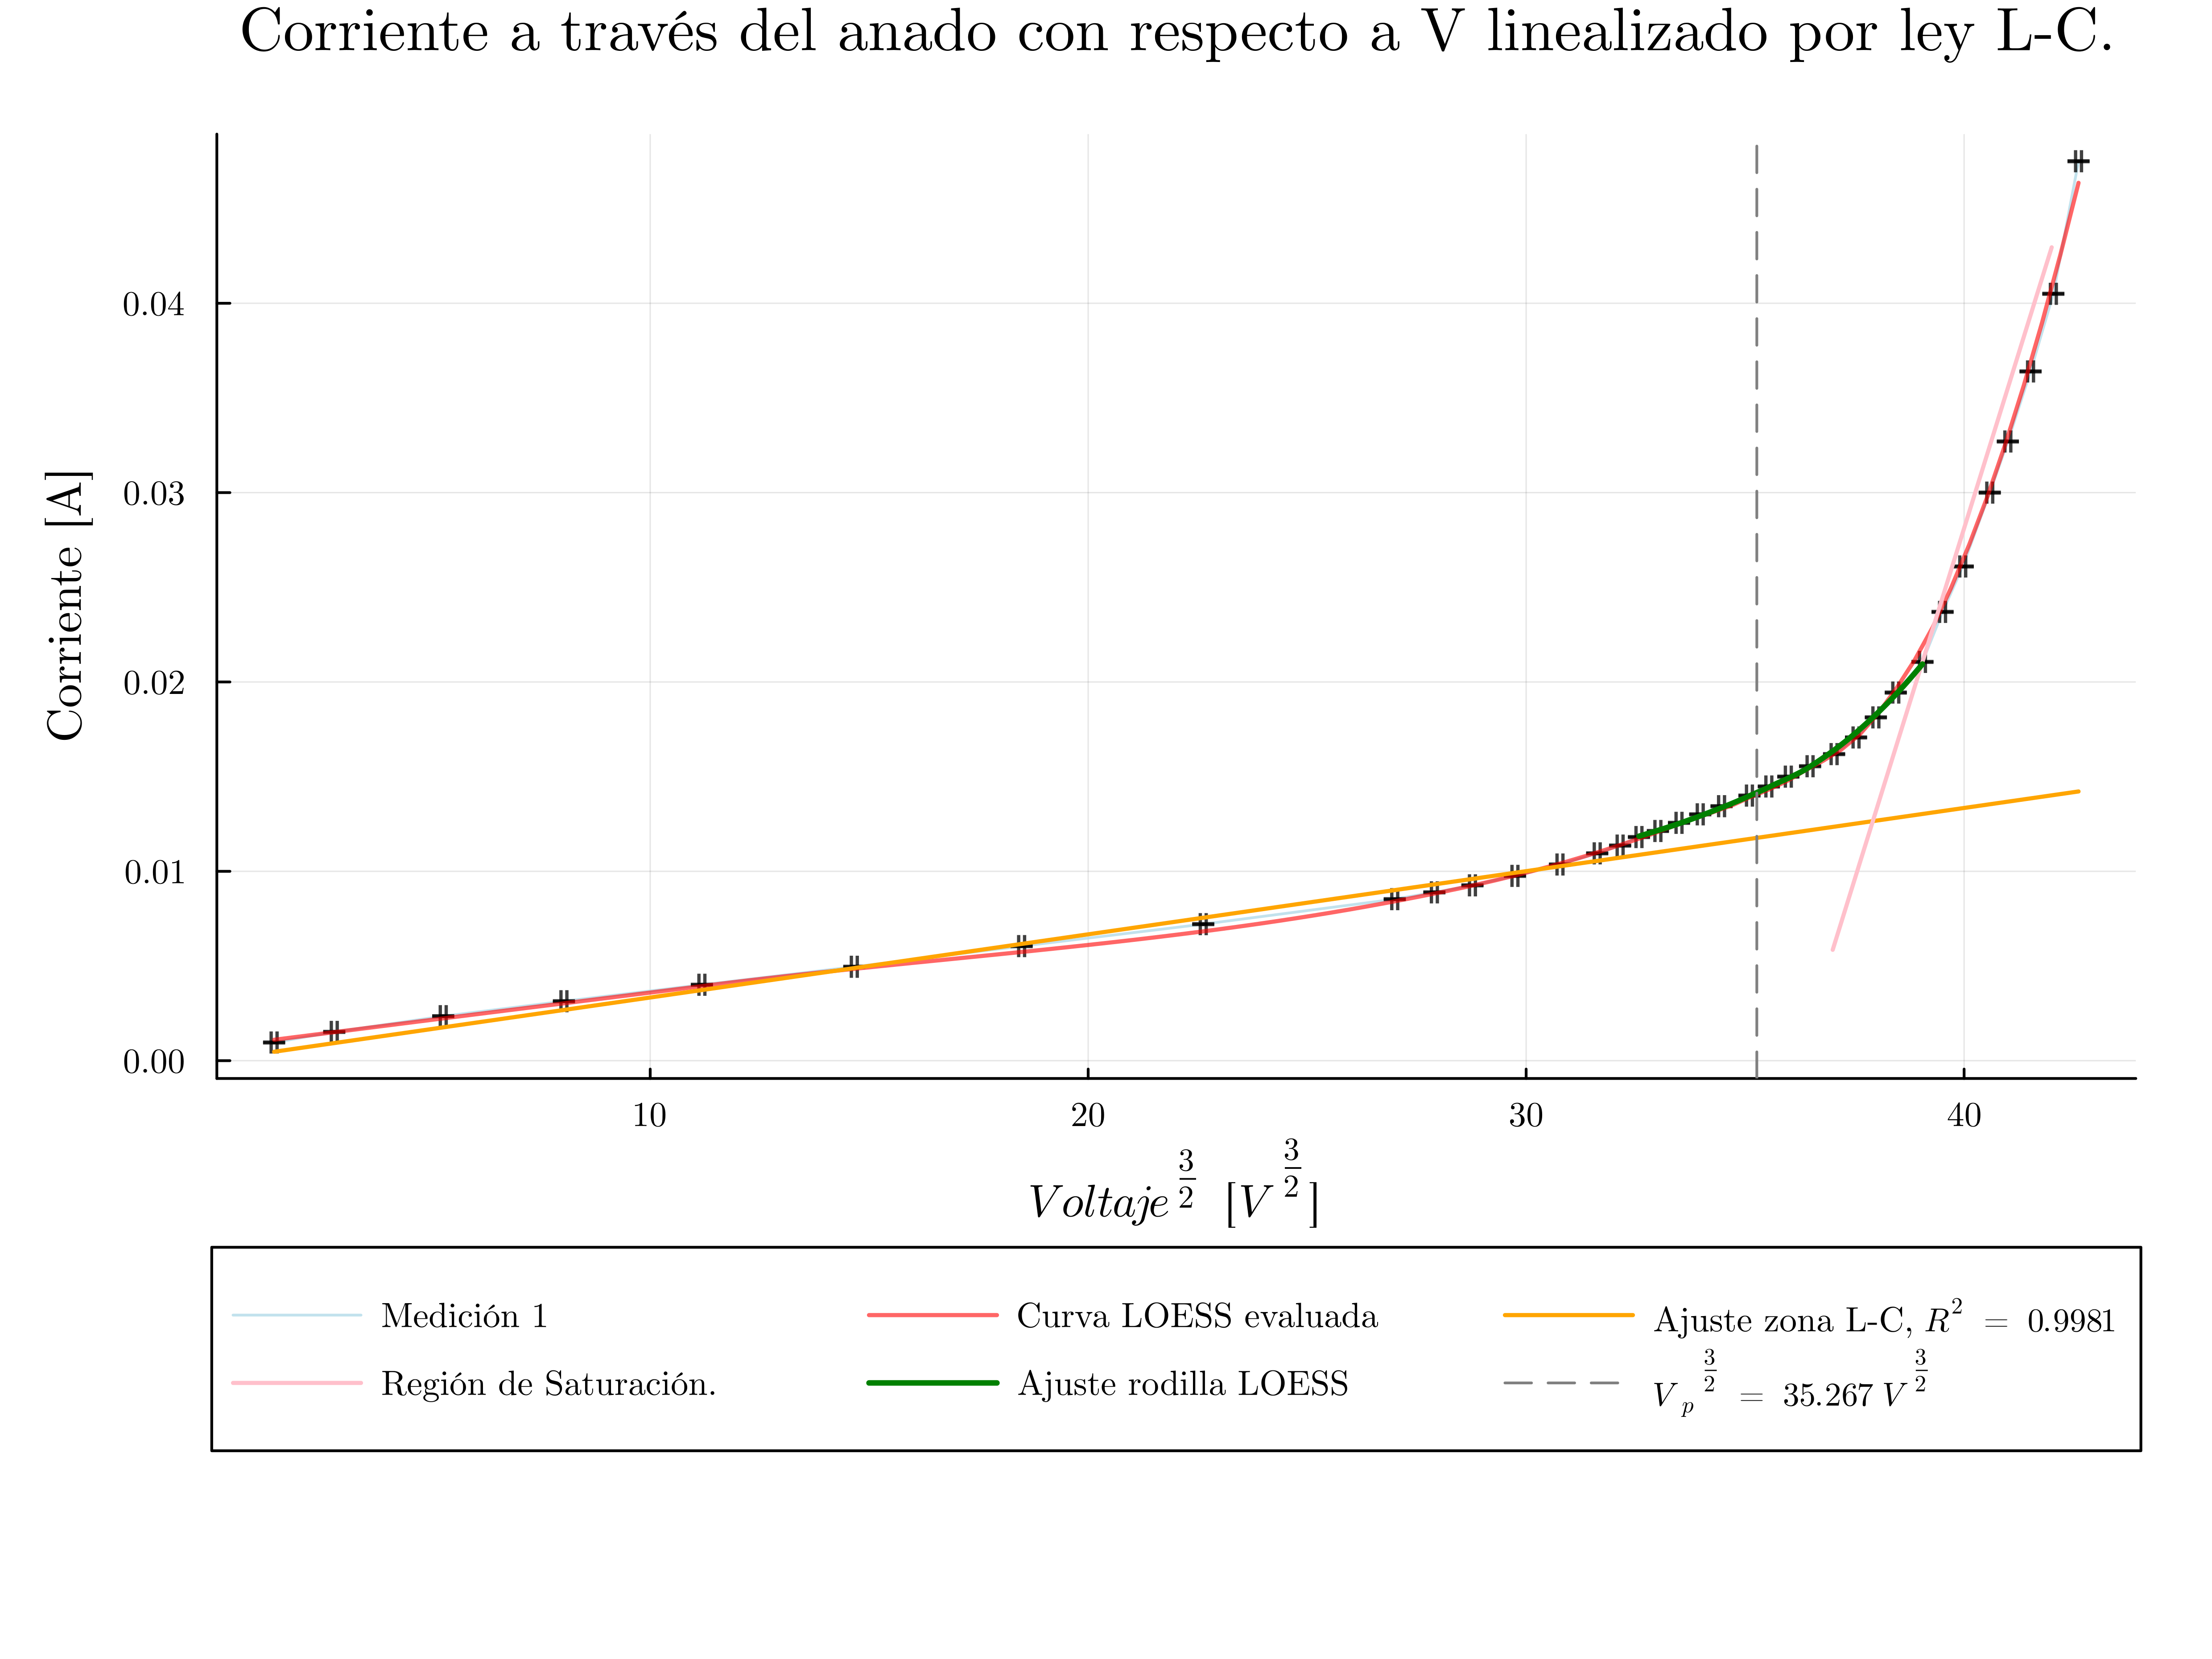
\includegraphics[width=\linewidth]{img/pot1.png}
	\caption{Barrido n°: 1}
	\label{fig:pot1}
	\end{subfigure}
	\hfill
	\begin{subfigure}[b]{0.49\textwidth}
		\centering
		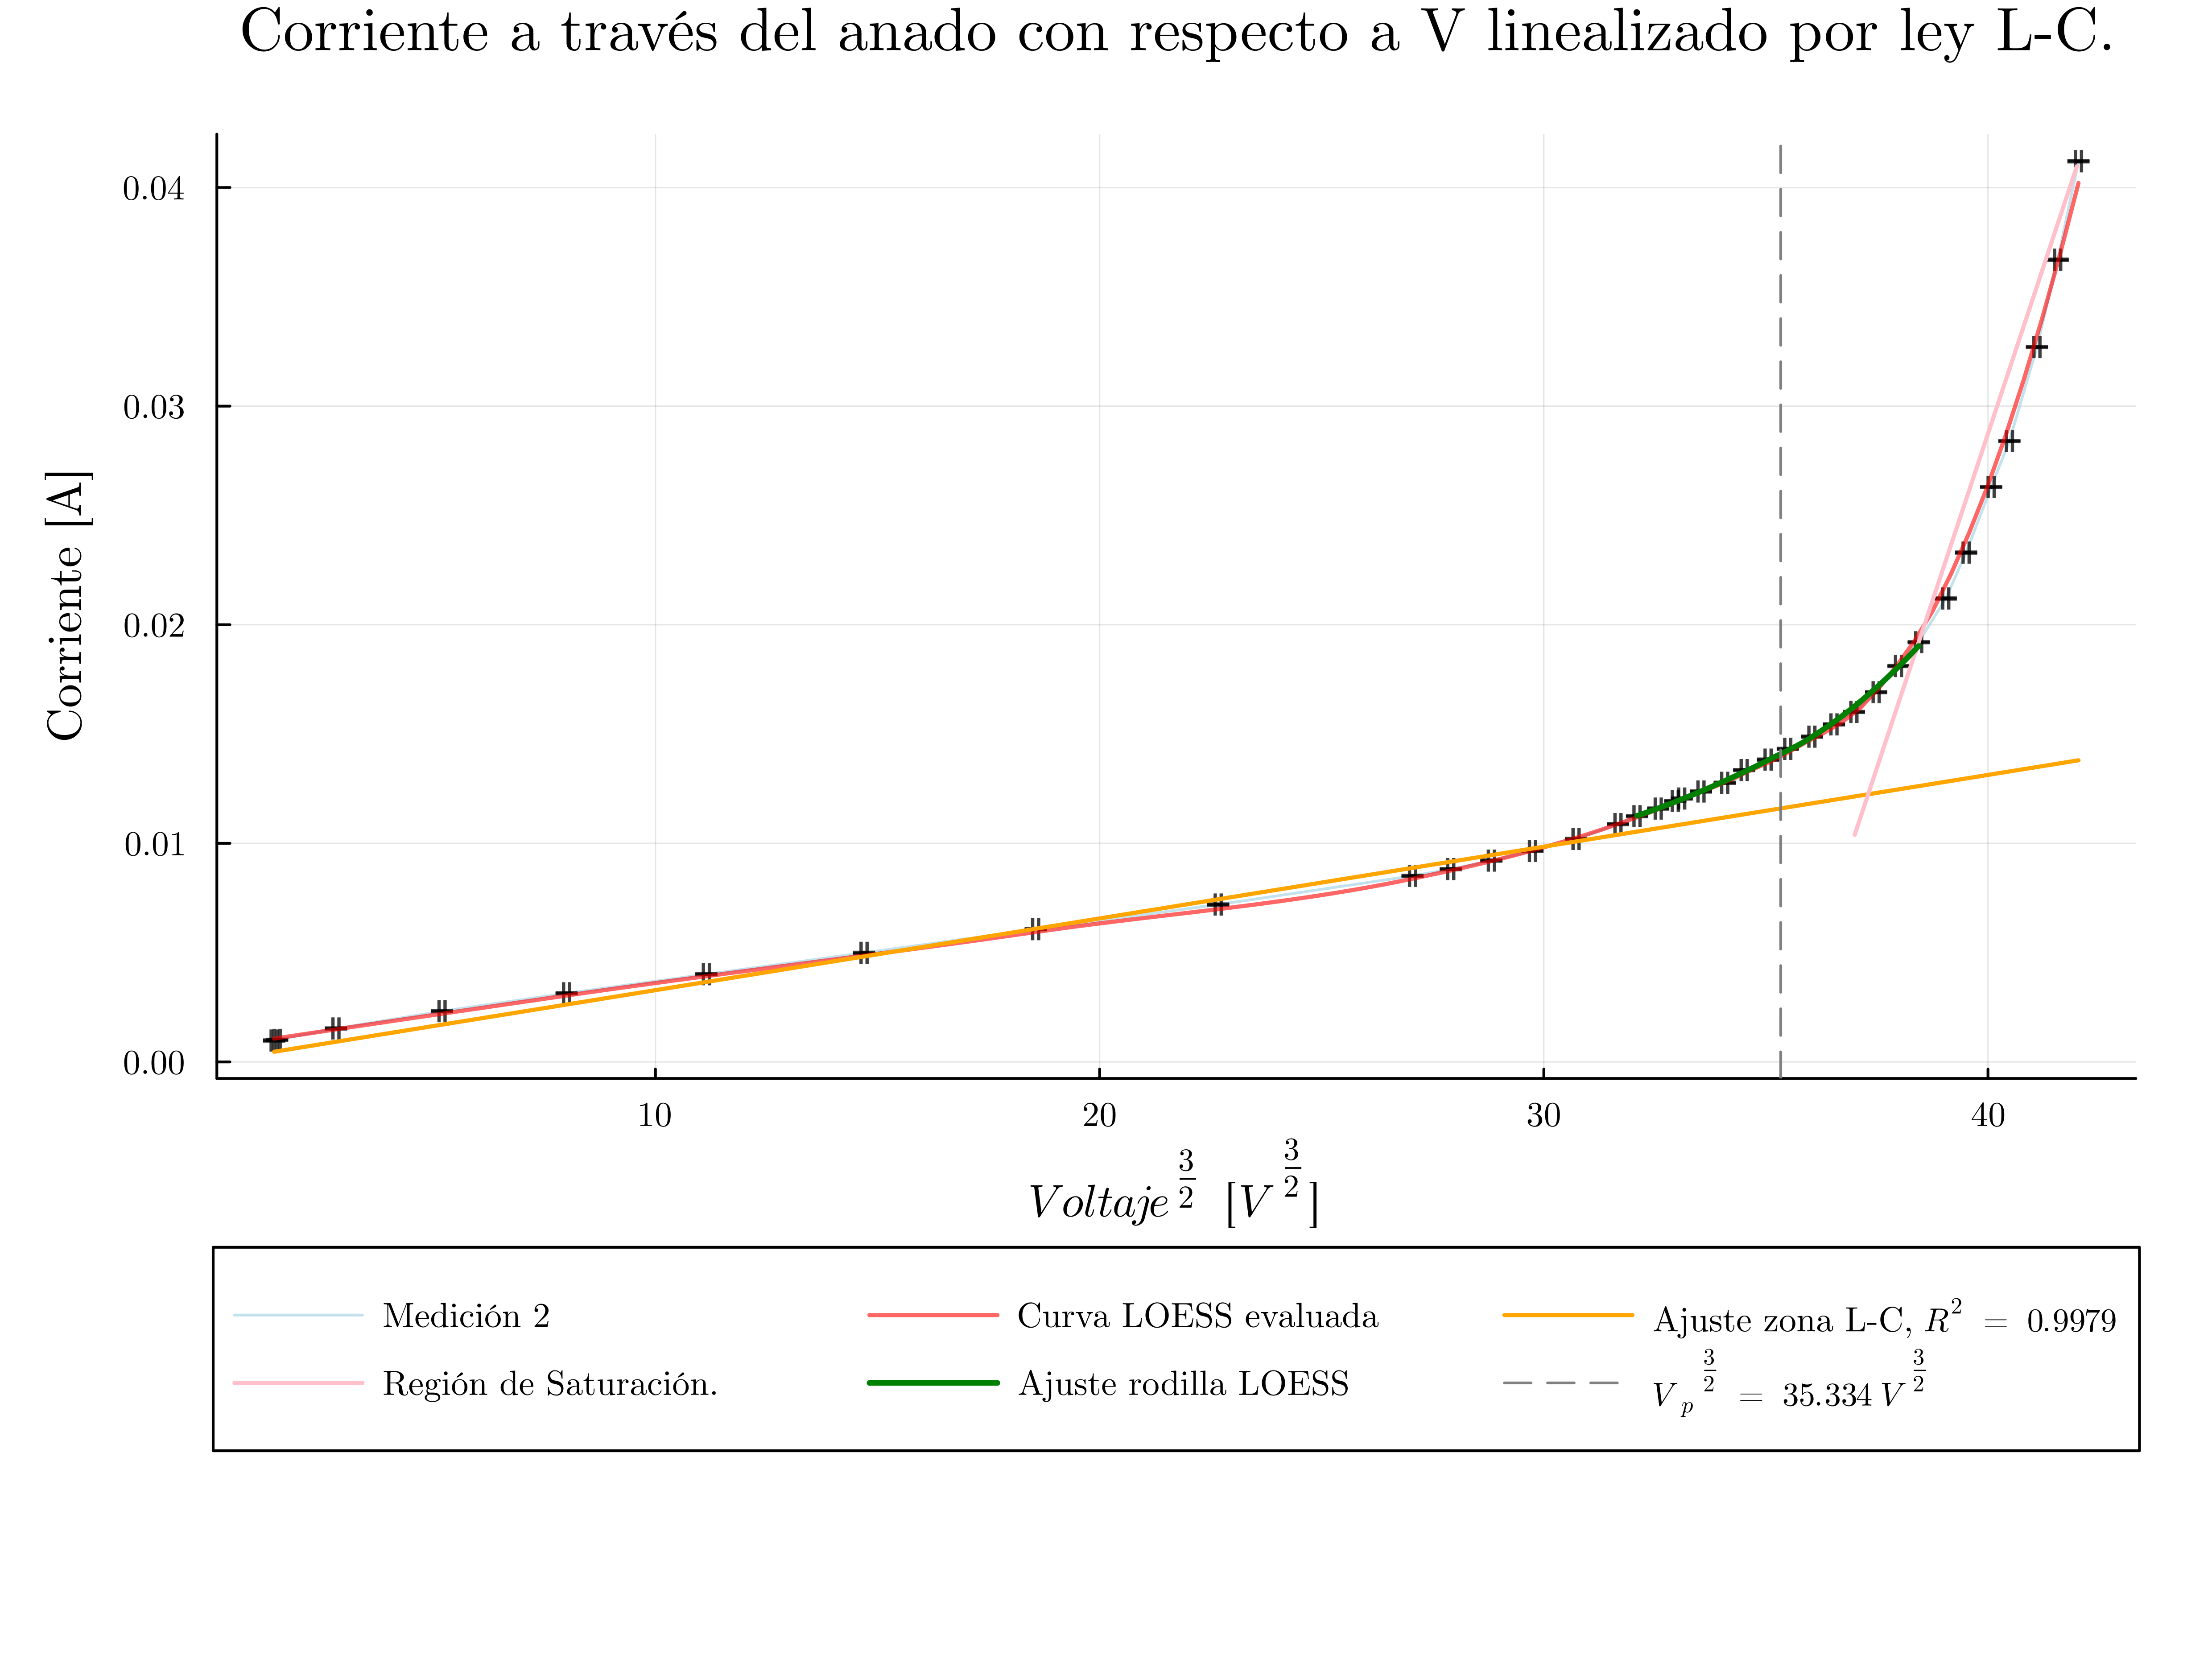
\includegraphics[width=\linewidth]{img/pot2.png}
		\caption{Barrido n°: 2}
		\label{fig:pot2}
	\end{subfigure}
		
\end{figure}

% segundo bloque de figuras
\begin{figure}[H]
	\ContinuedFloat
	\centering
	\begin{subfigure}[b]{0.49\textwidth}
		\centering
		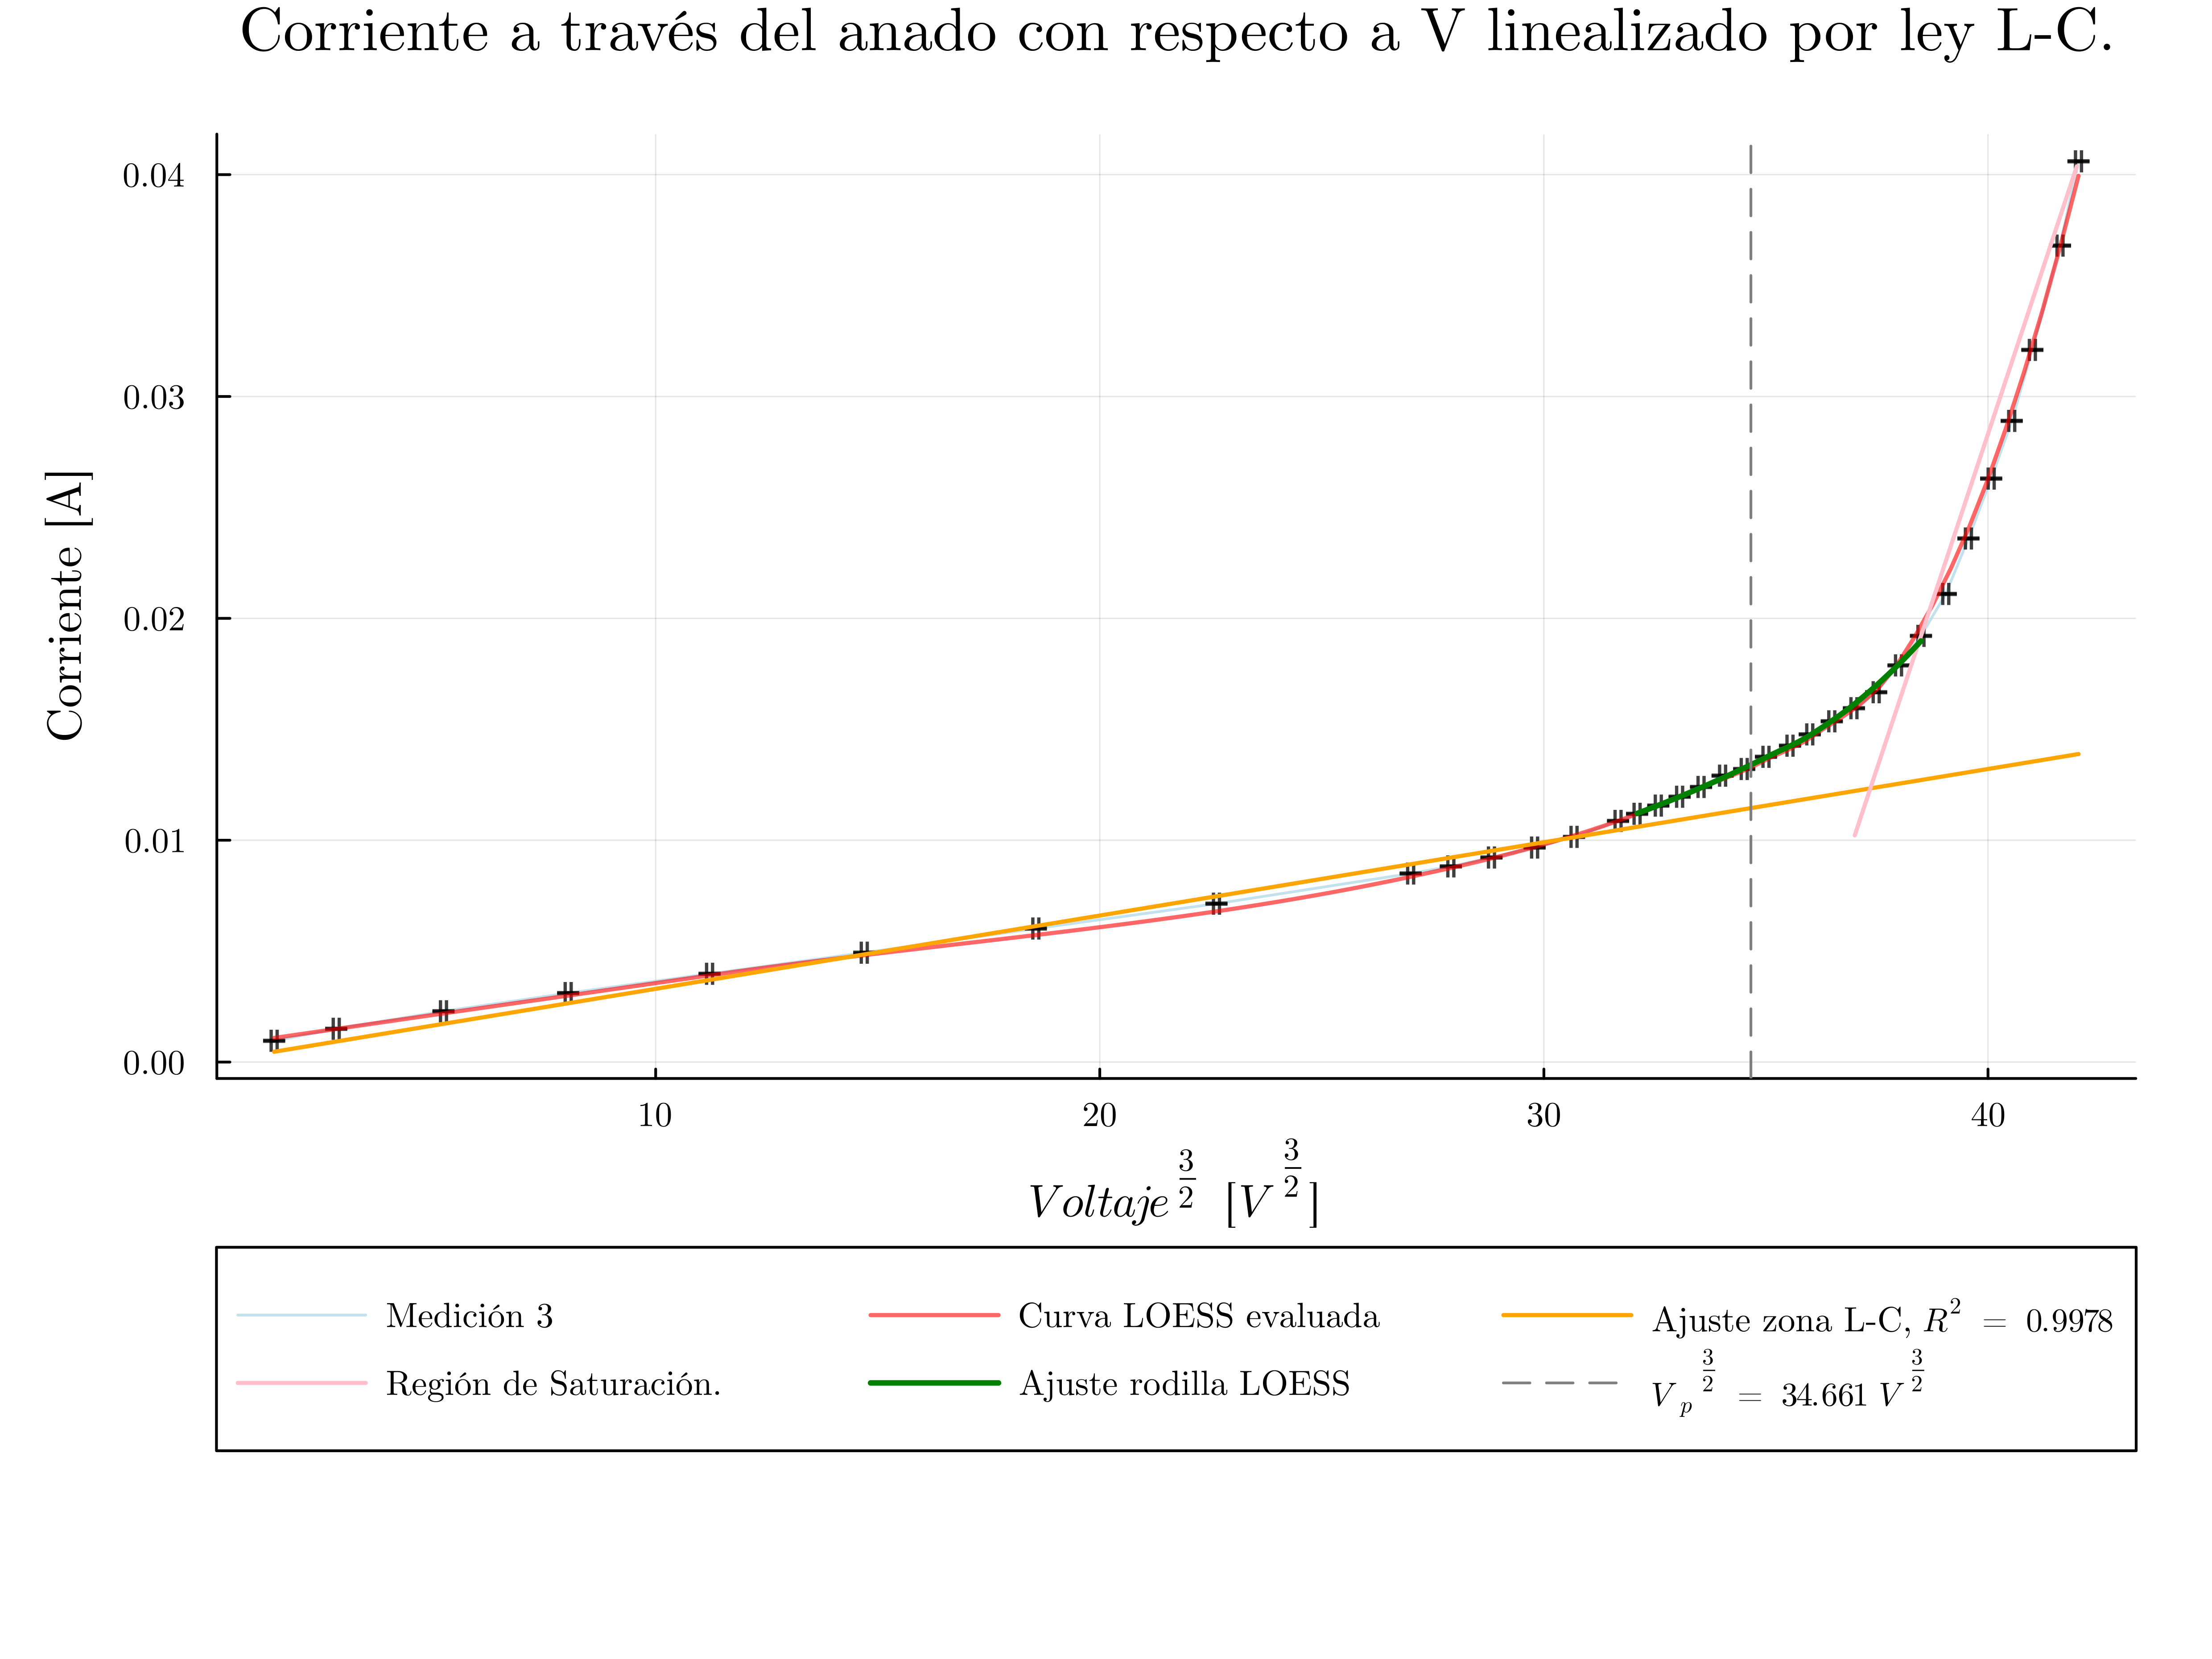
\includegraphics[width=\linewidth]{img/pot3.png}
		\caption{Barrido n°: 3}
		\label{fig:pot3}
	\end{subfigure}
	\hfill
	\begin{subfigure}[b]{0.49\textwidth}
		\centering
		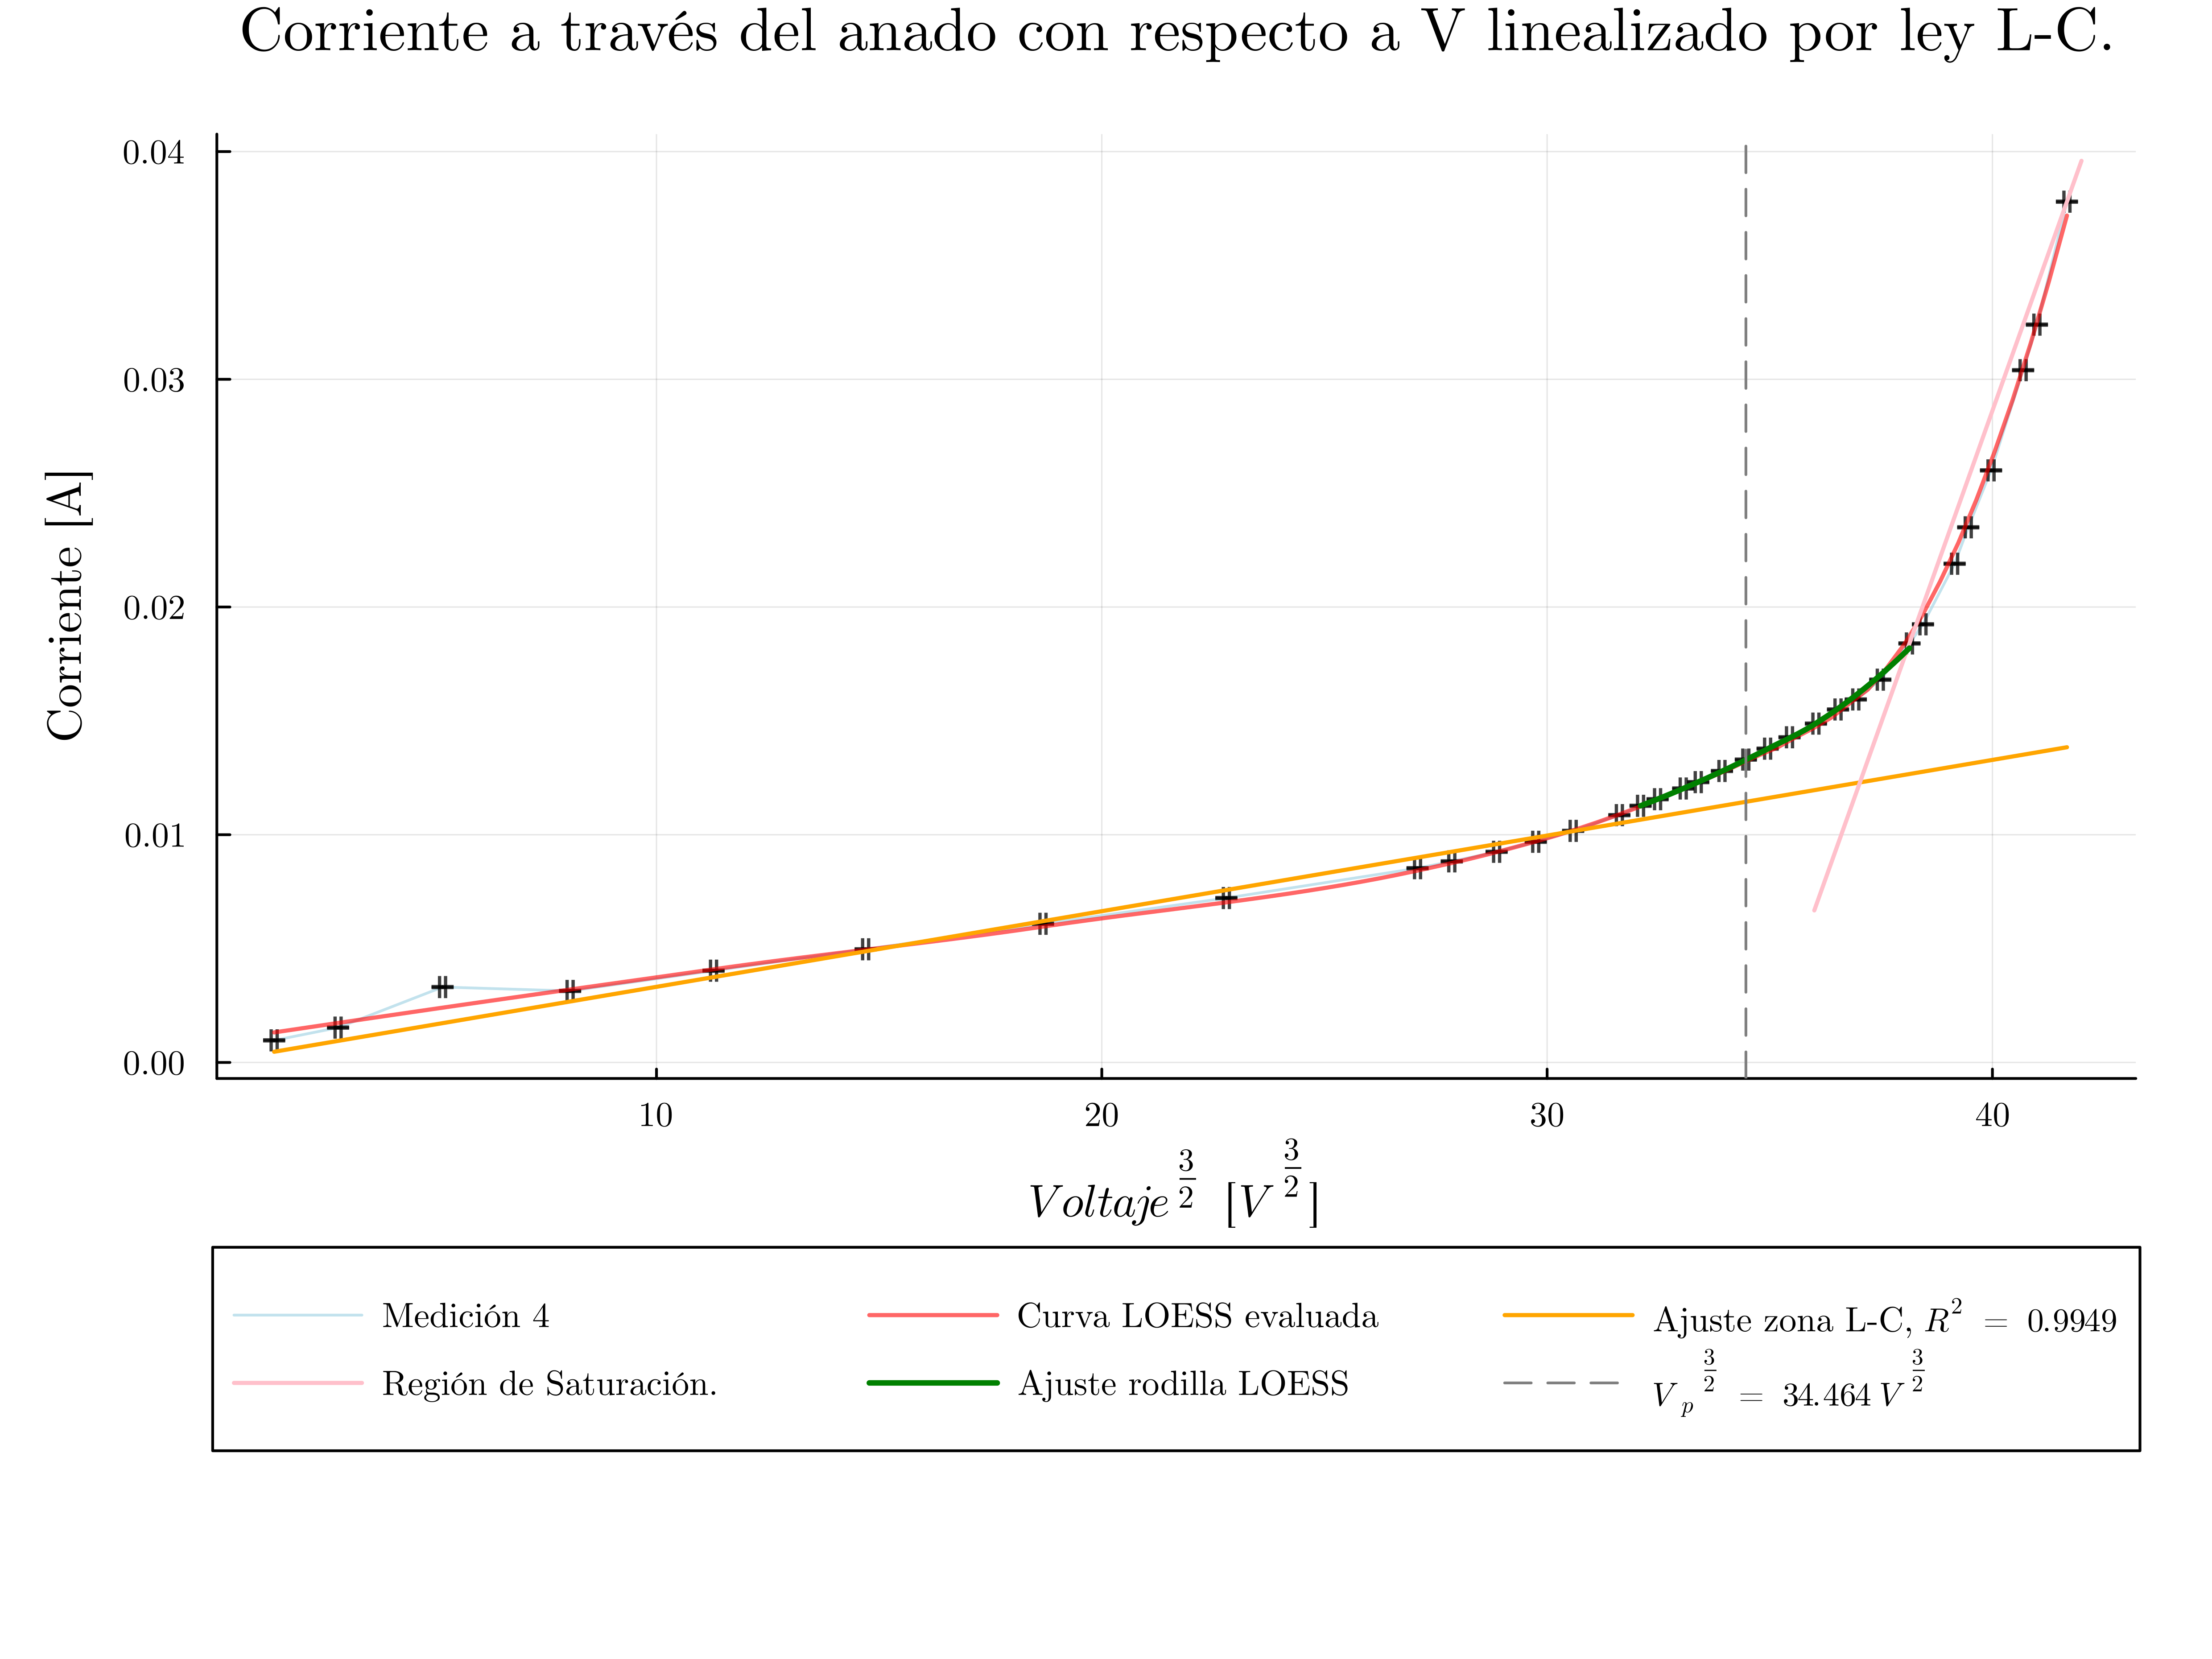
\includegraphics[width=\linewidth]{img/pot4.png}
		\caption{Barrido n°: 4}
		\label{fig:pot4}
	\end{subfigure}
	
\end{figure}

% teercer bloque de figuras
\begin{figure}[H]
	\ContinuedFloat % Indica que esta figura continúa de la anterior
	\centering
	\begin{subfigure}[b]{0.49\textwidth}
		\centering
		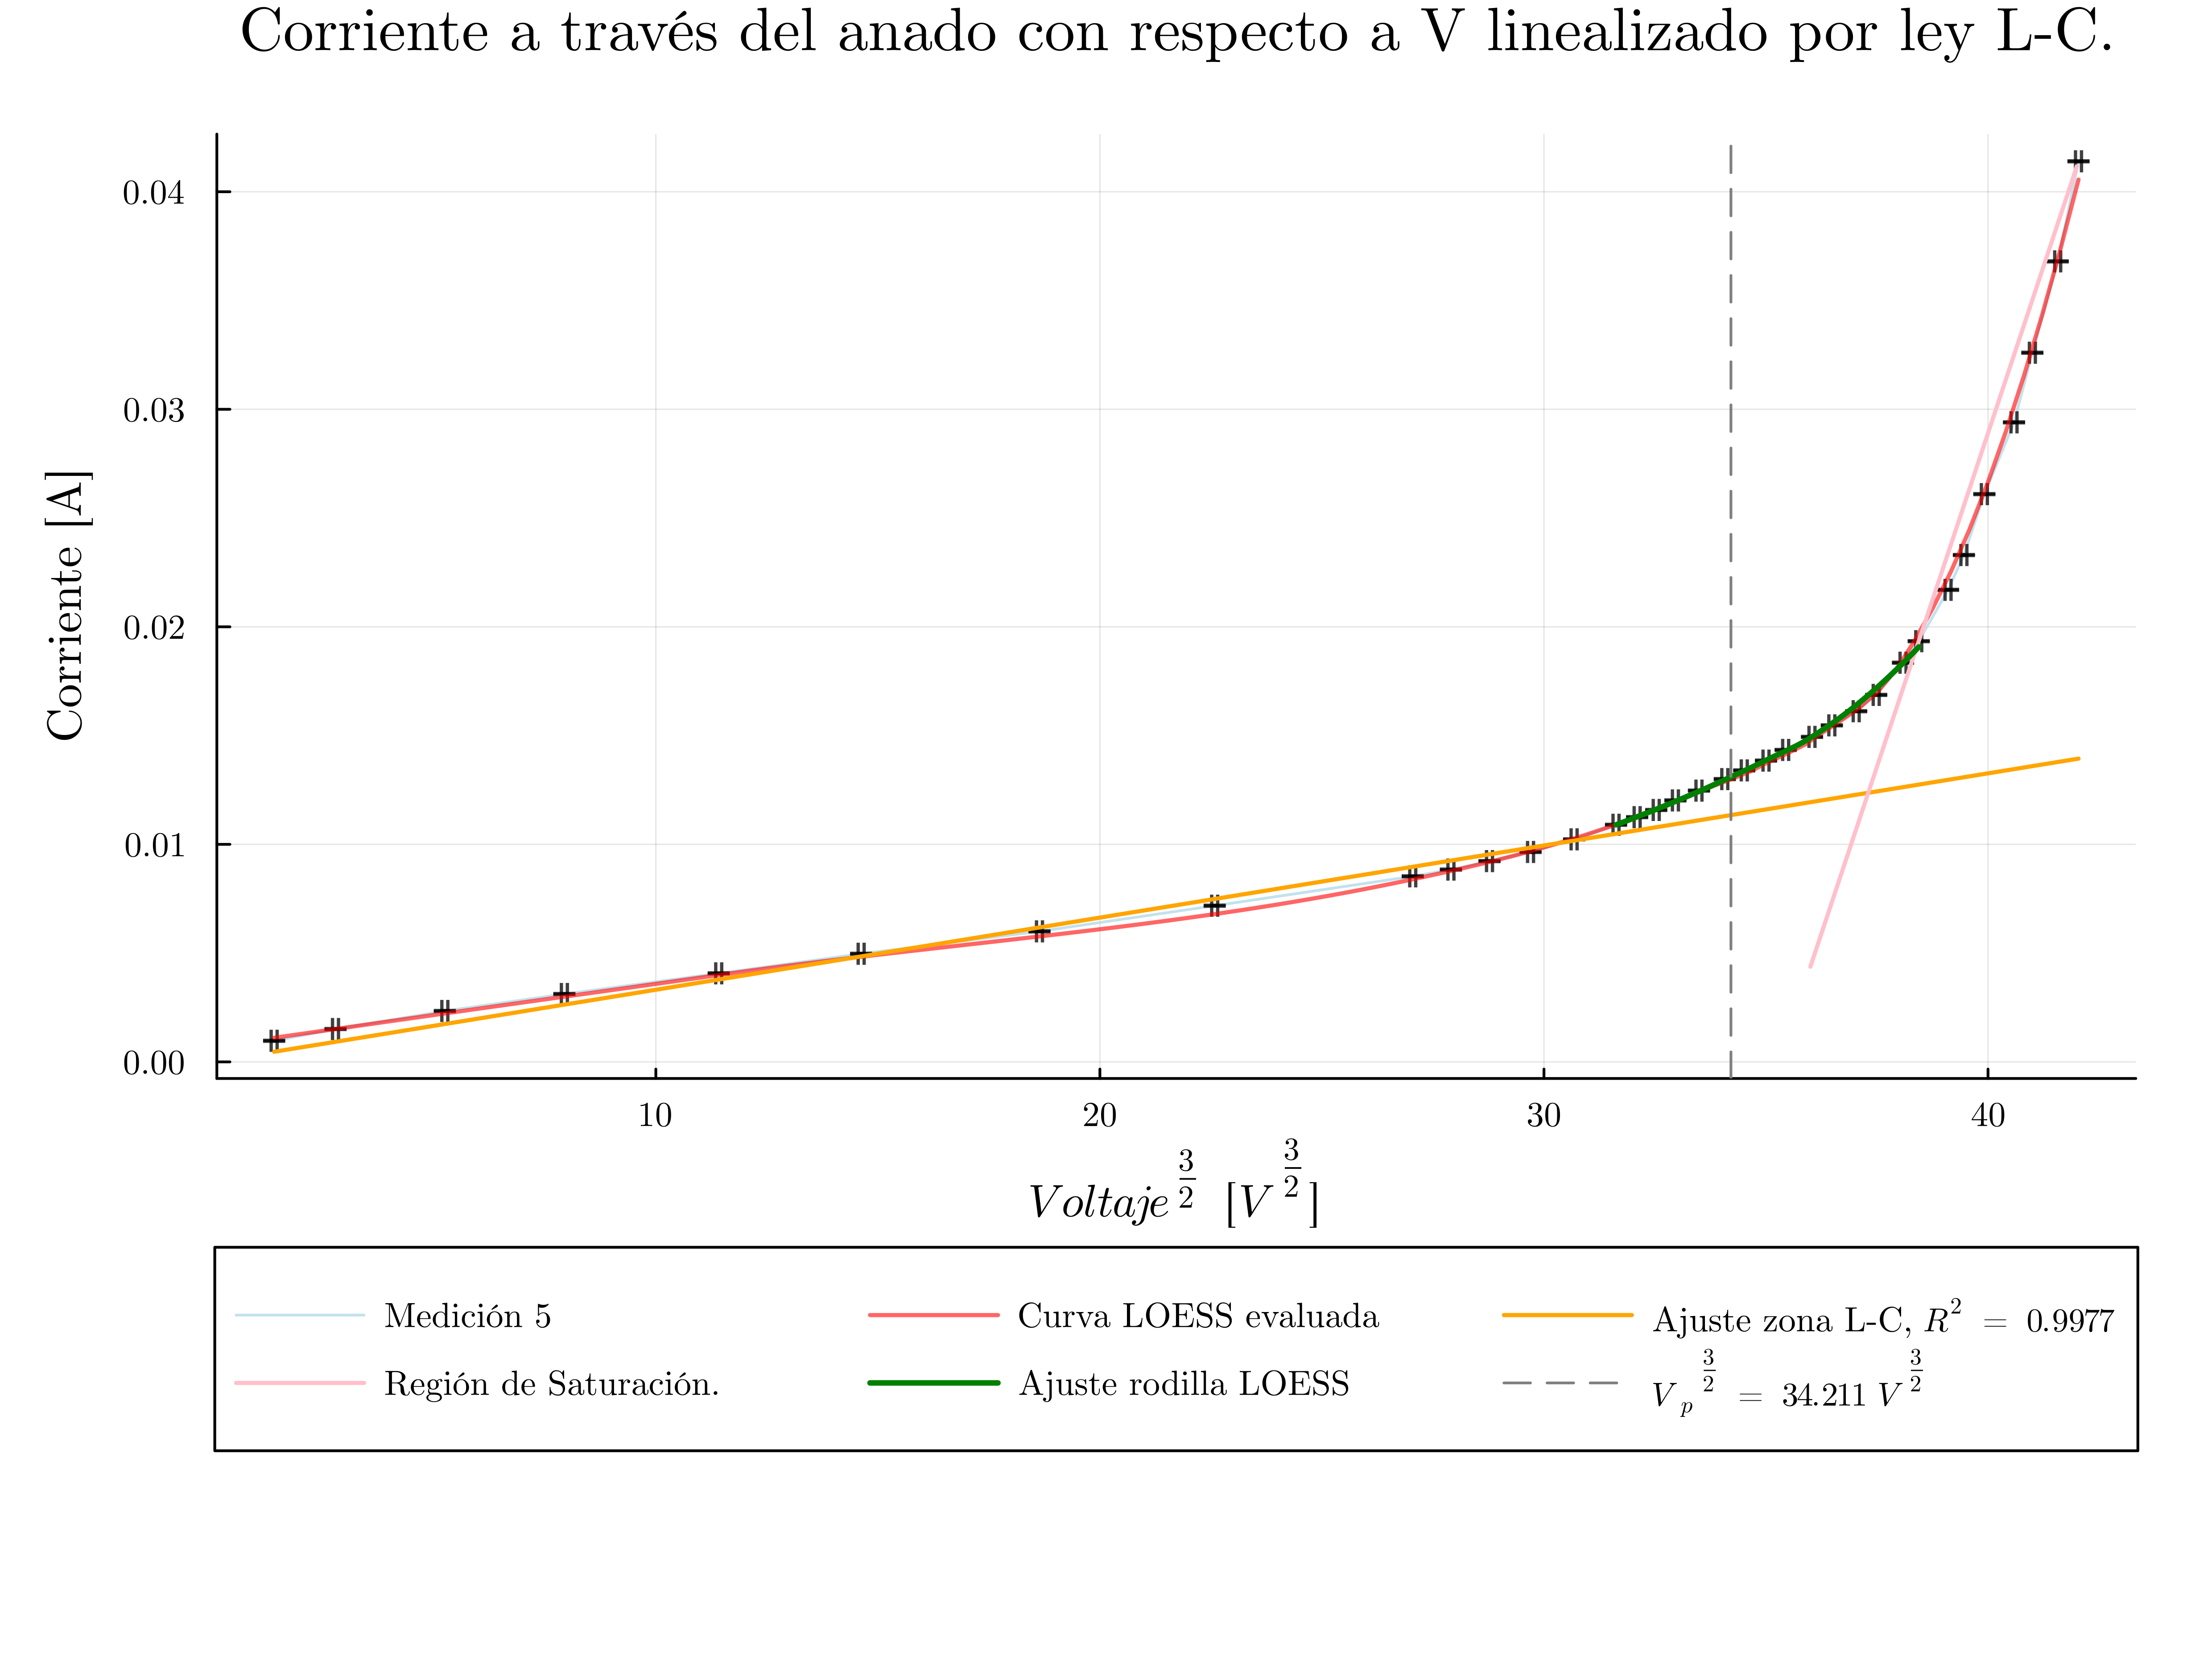
\includegraphics[width=\linewidth]{img/pot5.png}
		\caption{Barrido n°: 5}
		\label{fig:pot5}
	\end{subfigure}
	\hfill
	\begin{subfigure}[b]{0.49\textwidth}
		\centering
		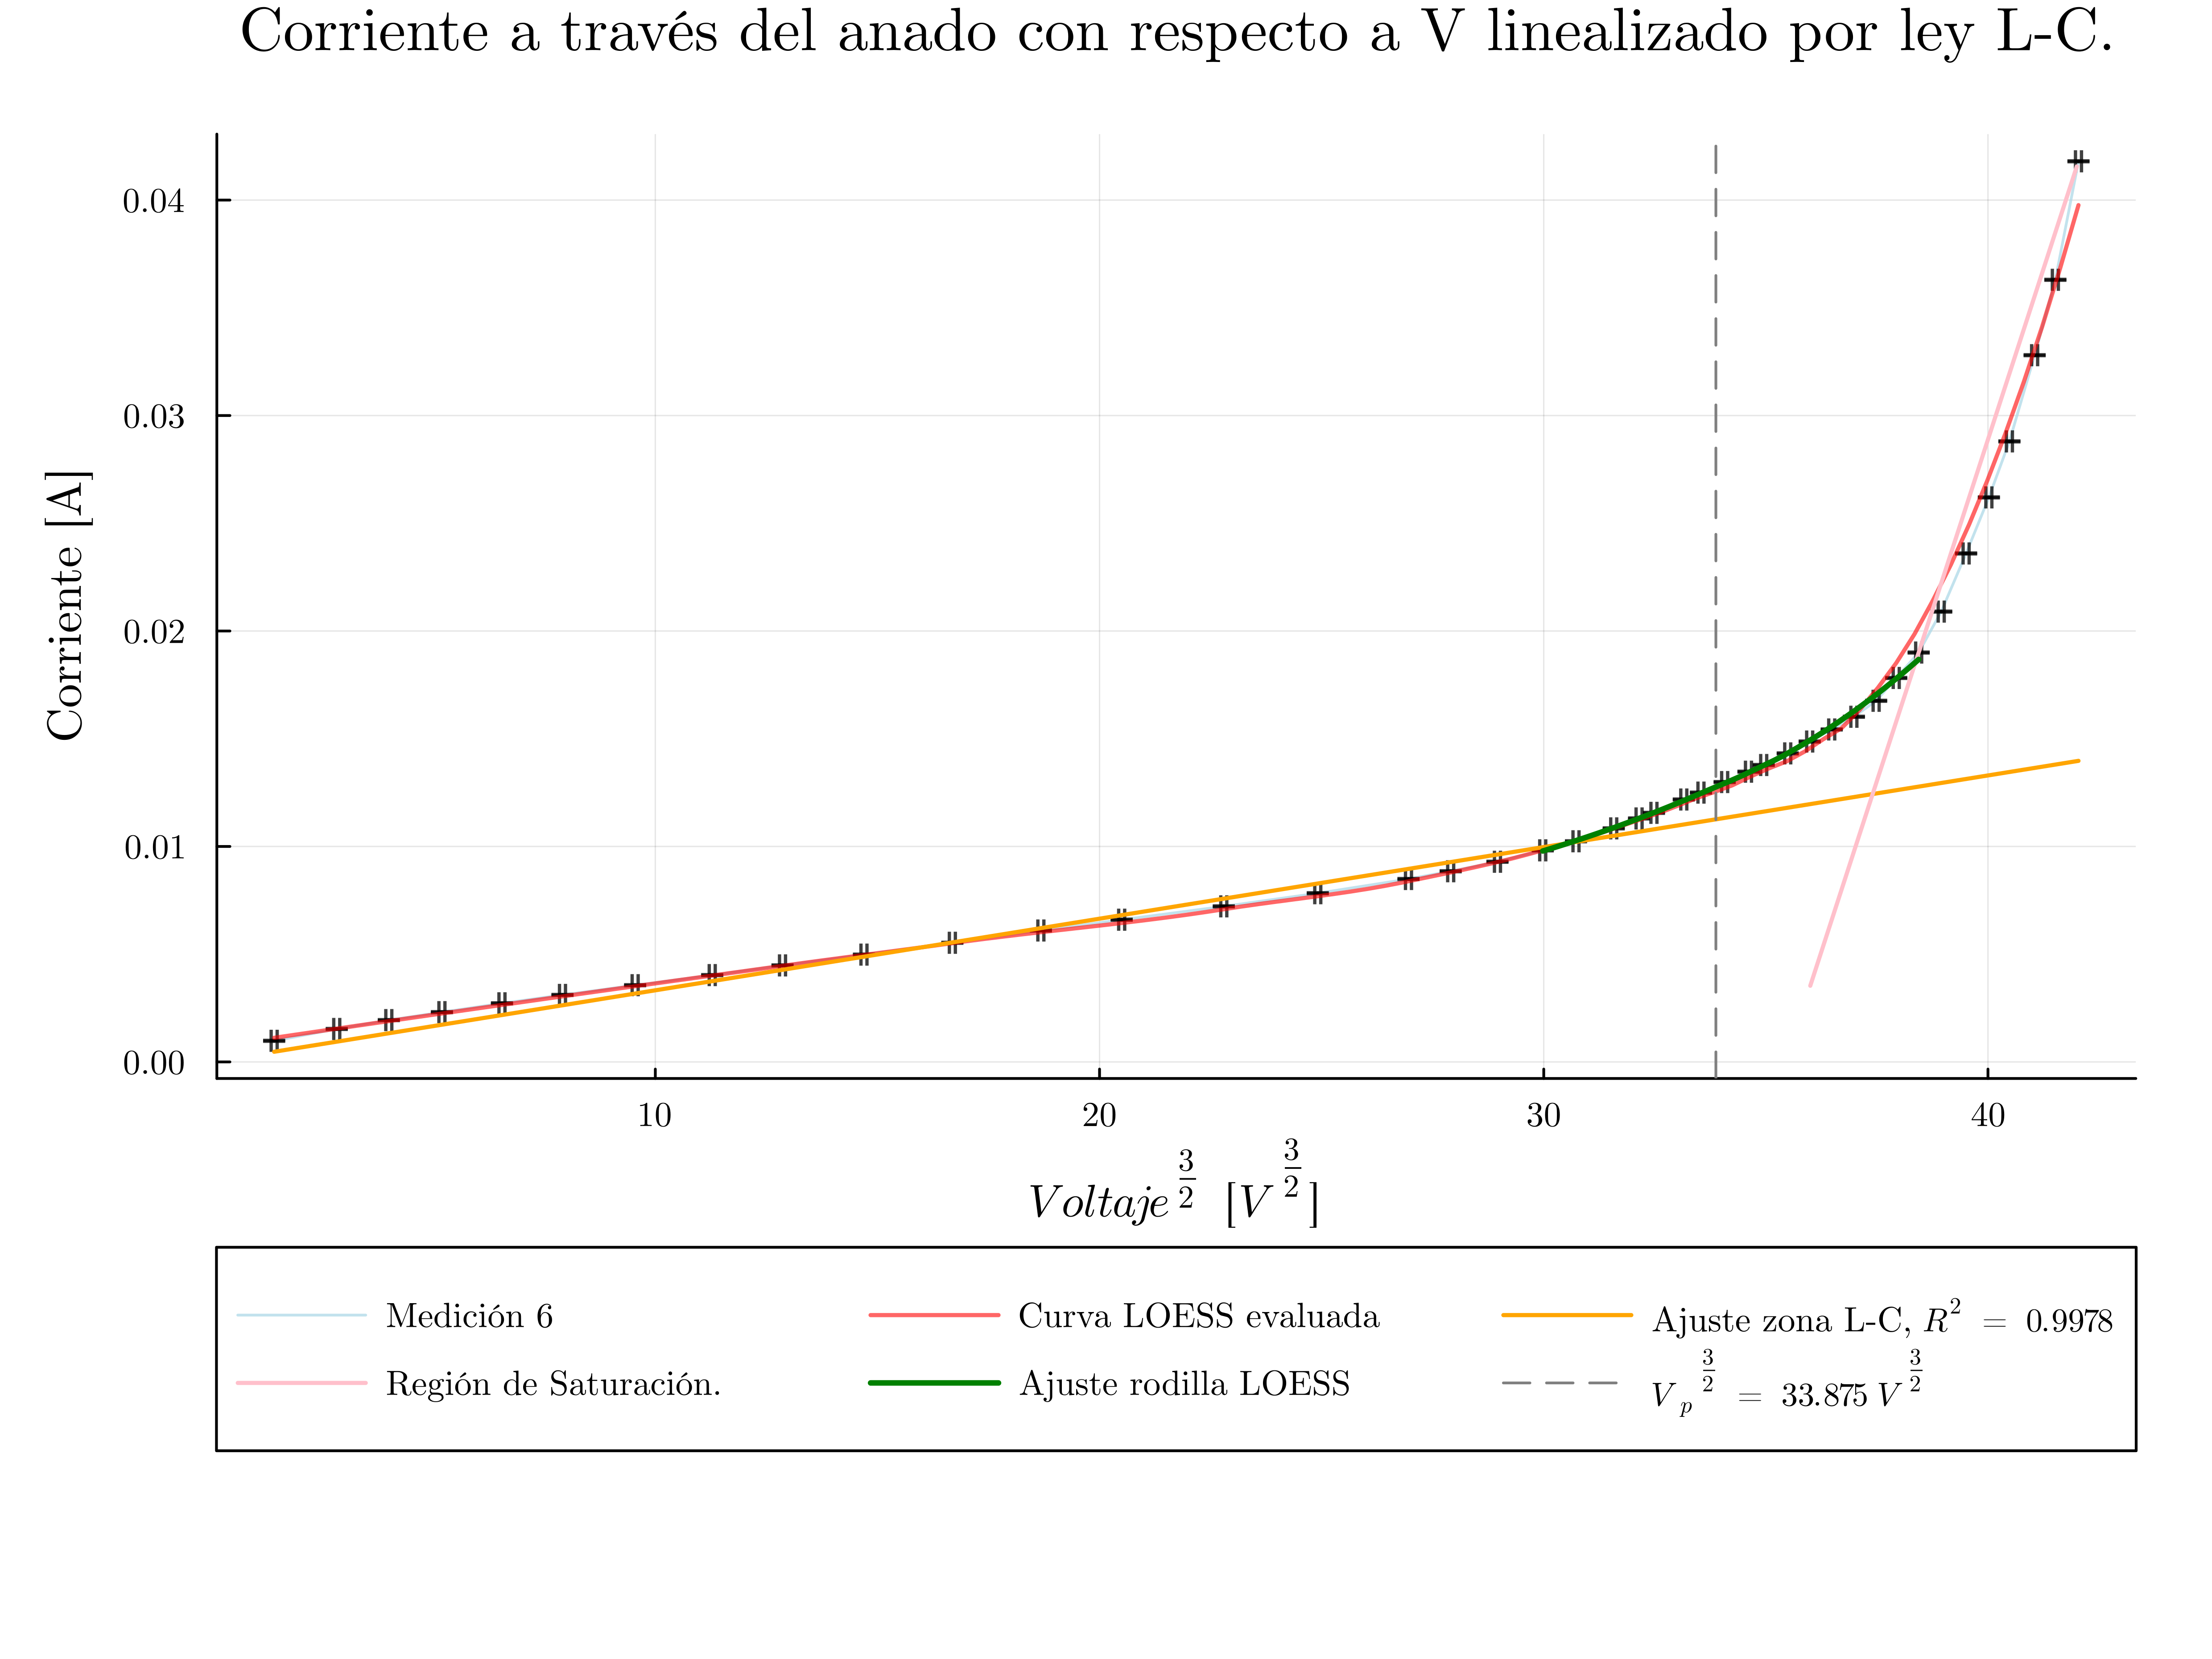
\includegraphics[width=\linewidth]{img/pot6.png}
		\caption{Barrido n°: 6}
		\label{fig:pot6}
	\end{subfigure}
	
\end{figure}

% cuarto bloque de figuras
\begin{figure}[H]
	\ContinuedFloat % Indica que esta figura continúa de la anterior
	\centering
	\begin{subfigure}[b]{0.49\textwidth}
		\centering
		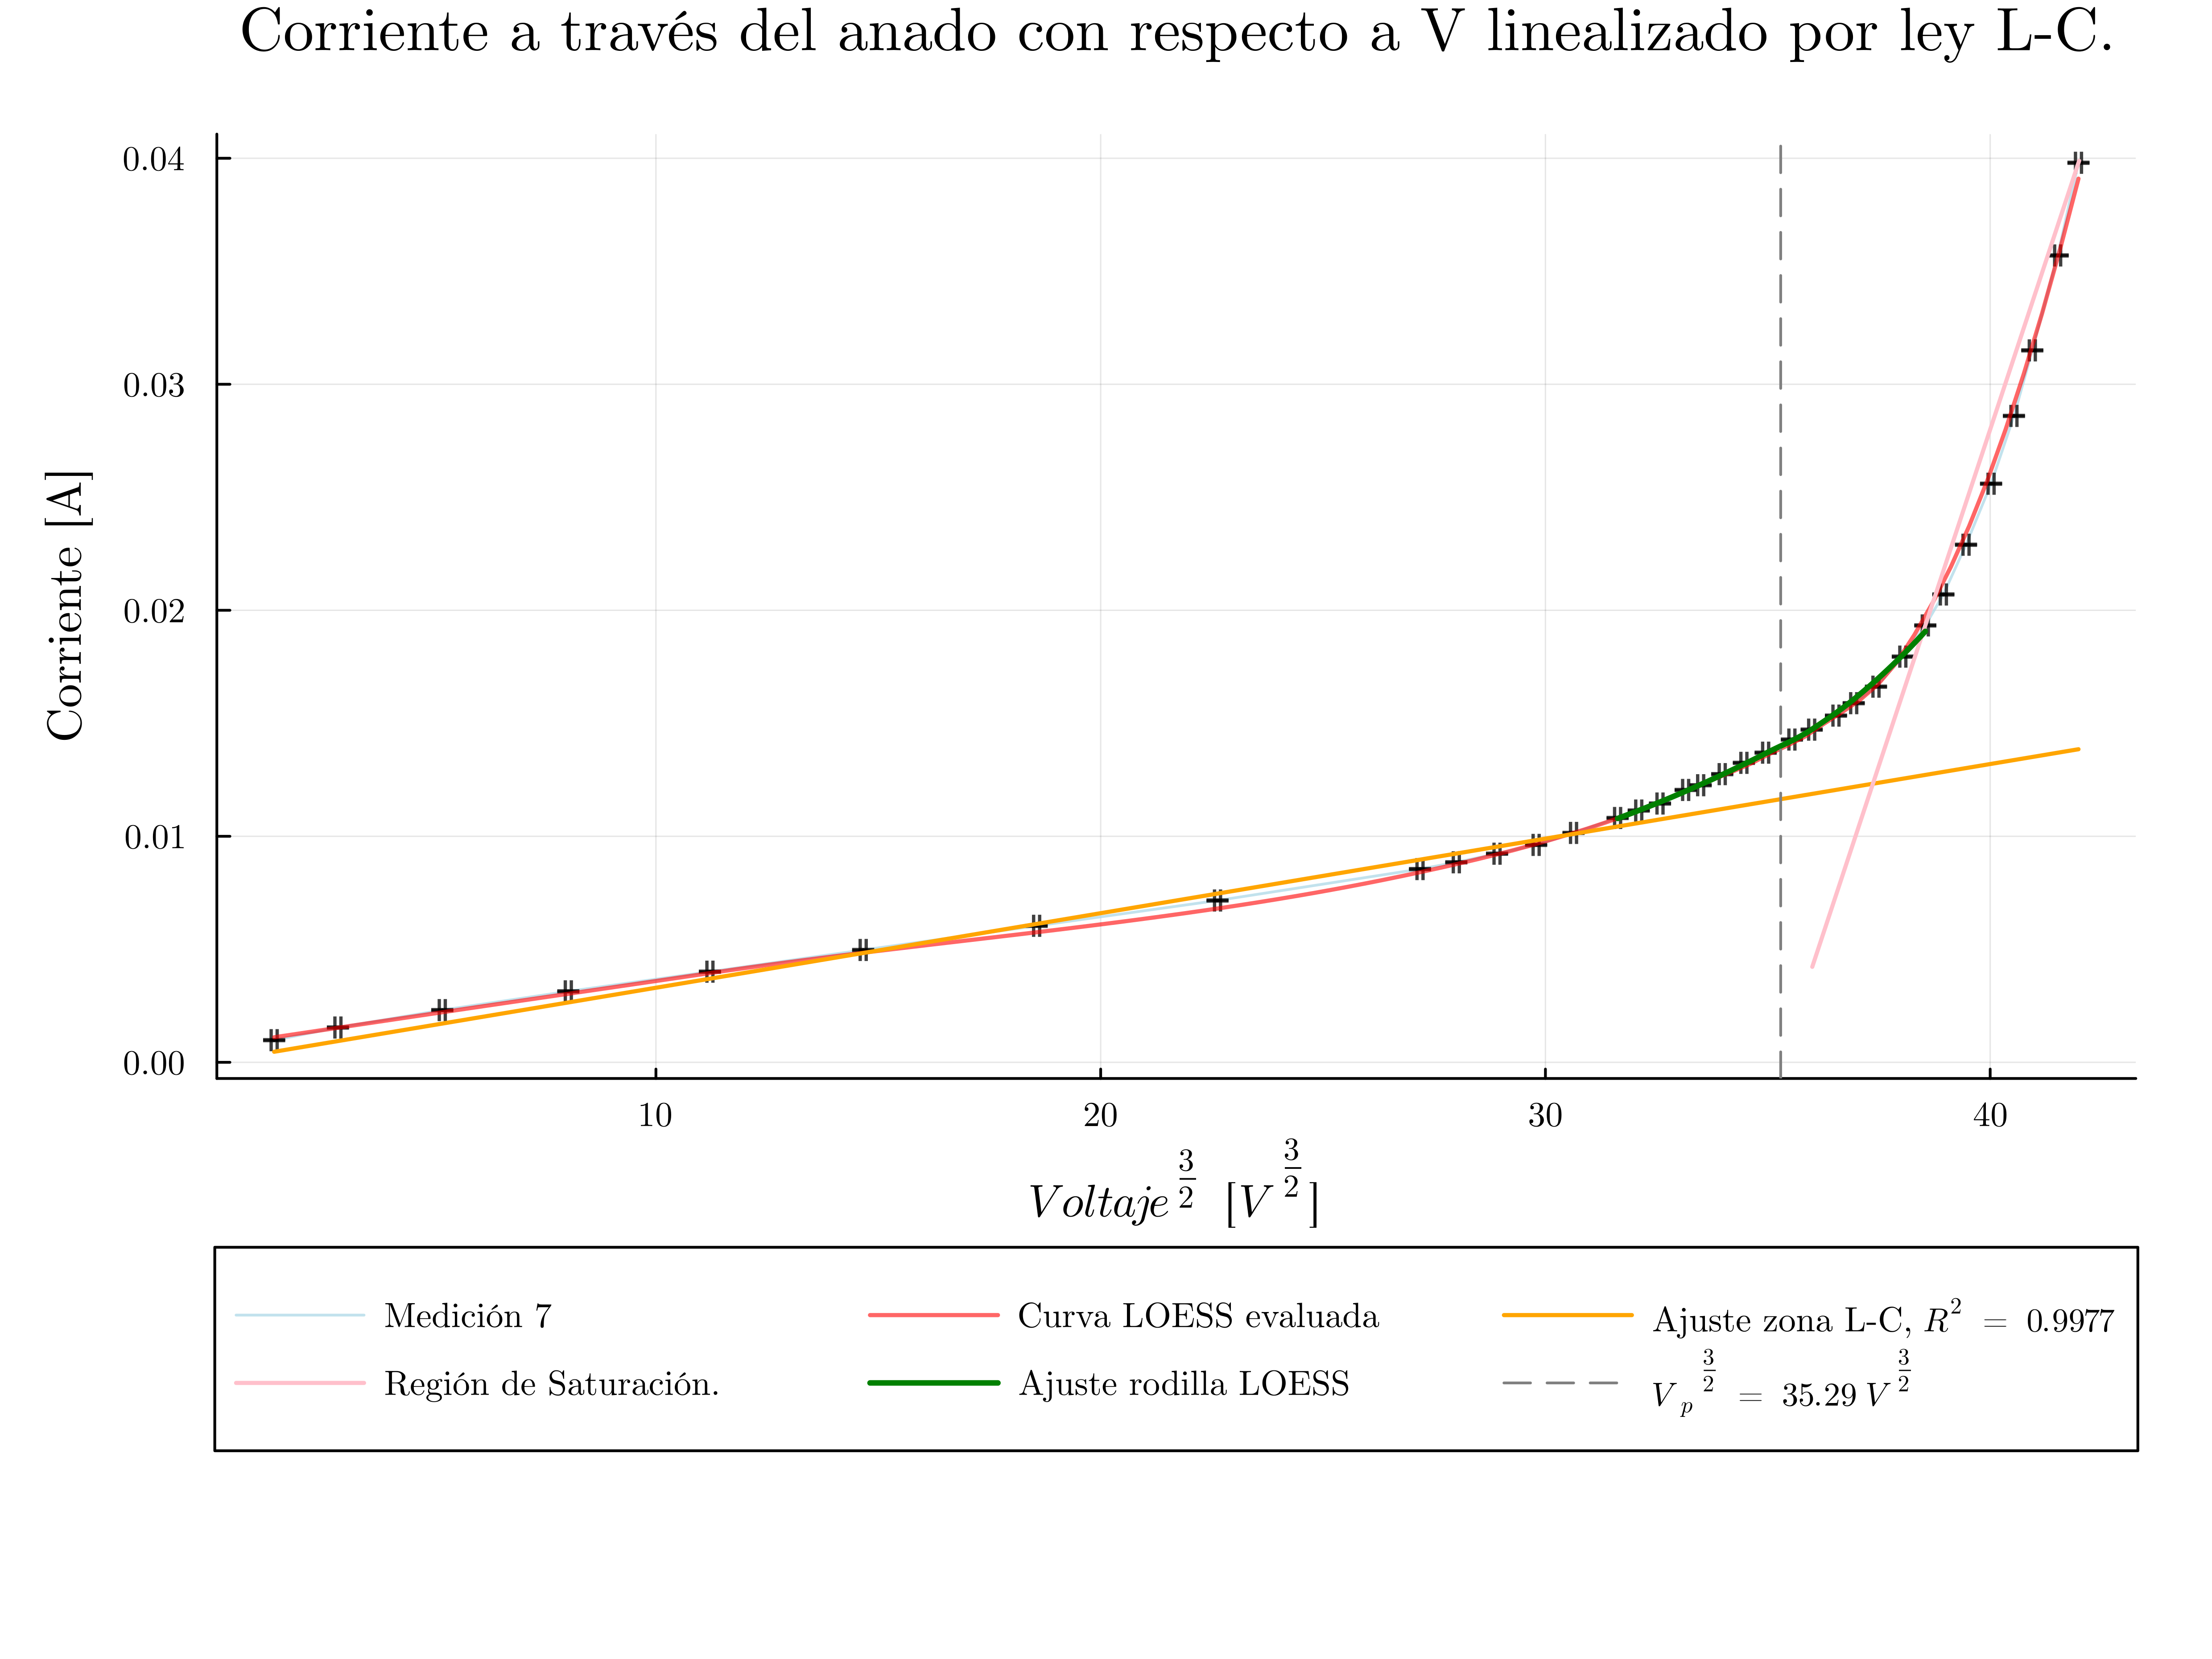
\includegraphics[width=\linewidth]{img/pot7.png}
		\caption{Barrido n°: 7}
		\label{fig:pot7}
	\end{subfigure}
	\hfill
	\begin{subfigure}[b]{0.49\textwidth}
		\centering
		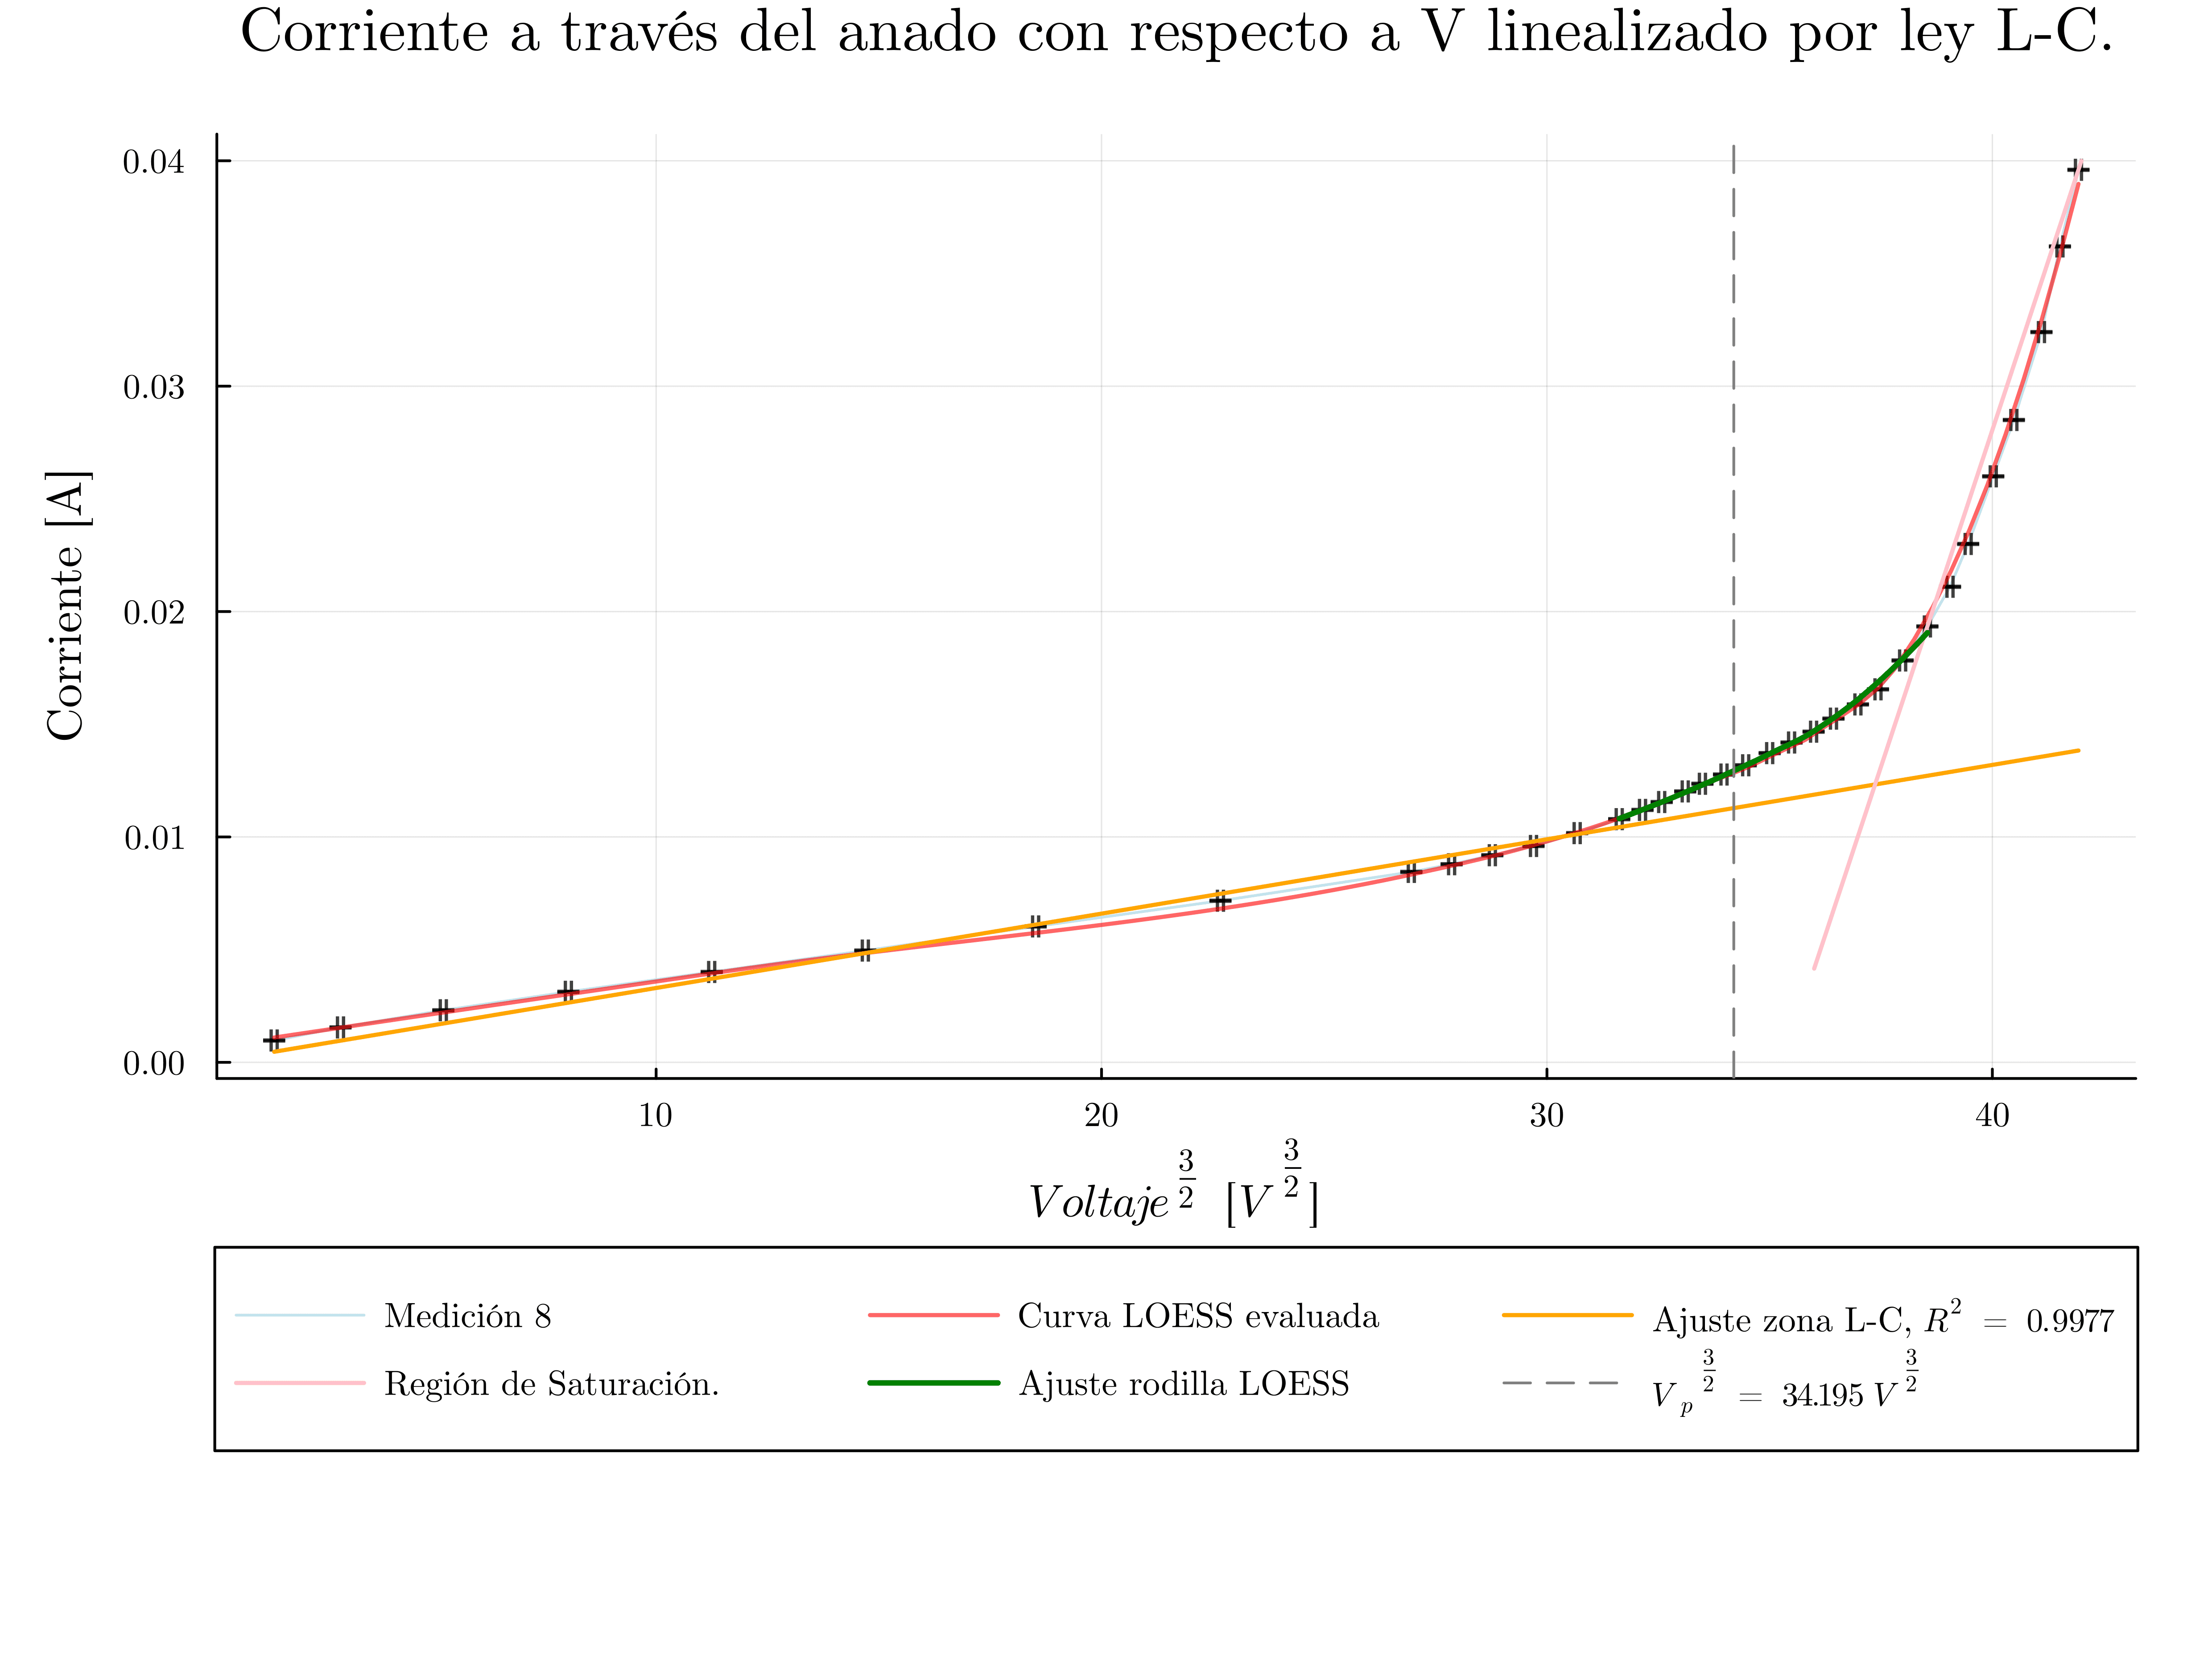
\includegraphics[width=\linewidth]{img/pot8.png}
		\caption{Barrido n°: 8}
		\label{fig:pot8}
	\end{subfigure}
\end{figure}


% Últimas figuras
\begin{figure}[H]
	\ContinuedFloat % Sigue con la misma numeración y caption
	\centering
	\begin{subfigure}[b]{0.49\textwidth}
		\centering
		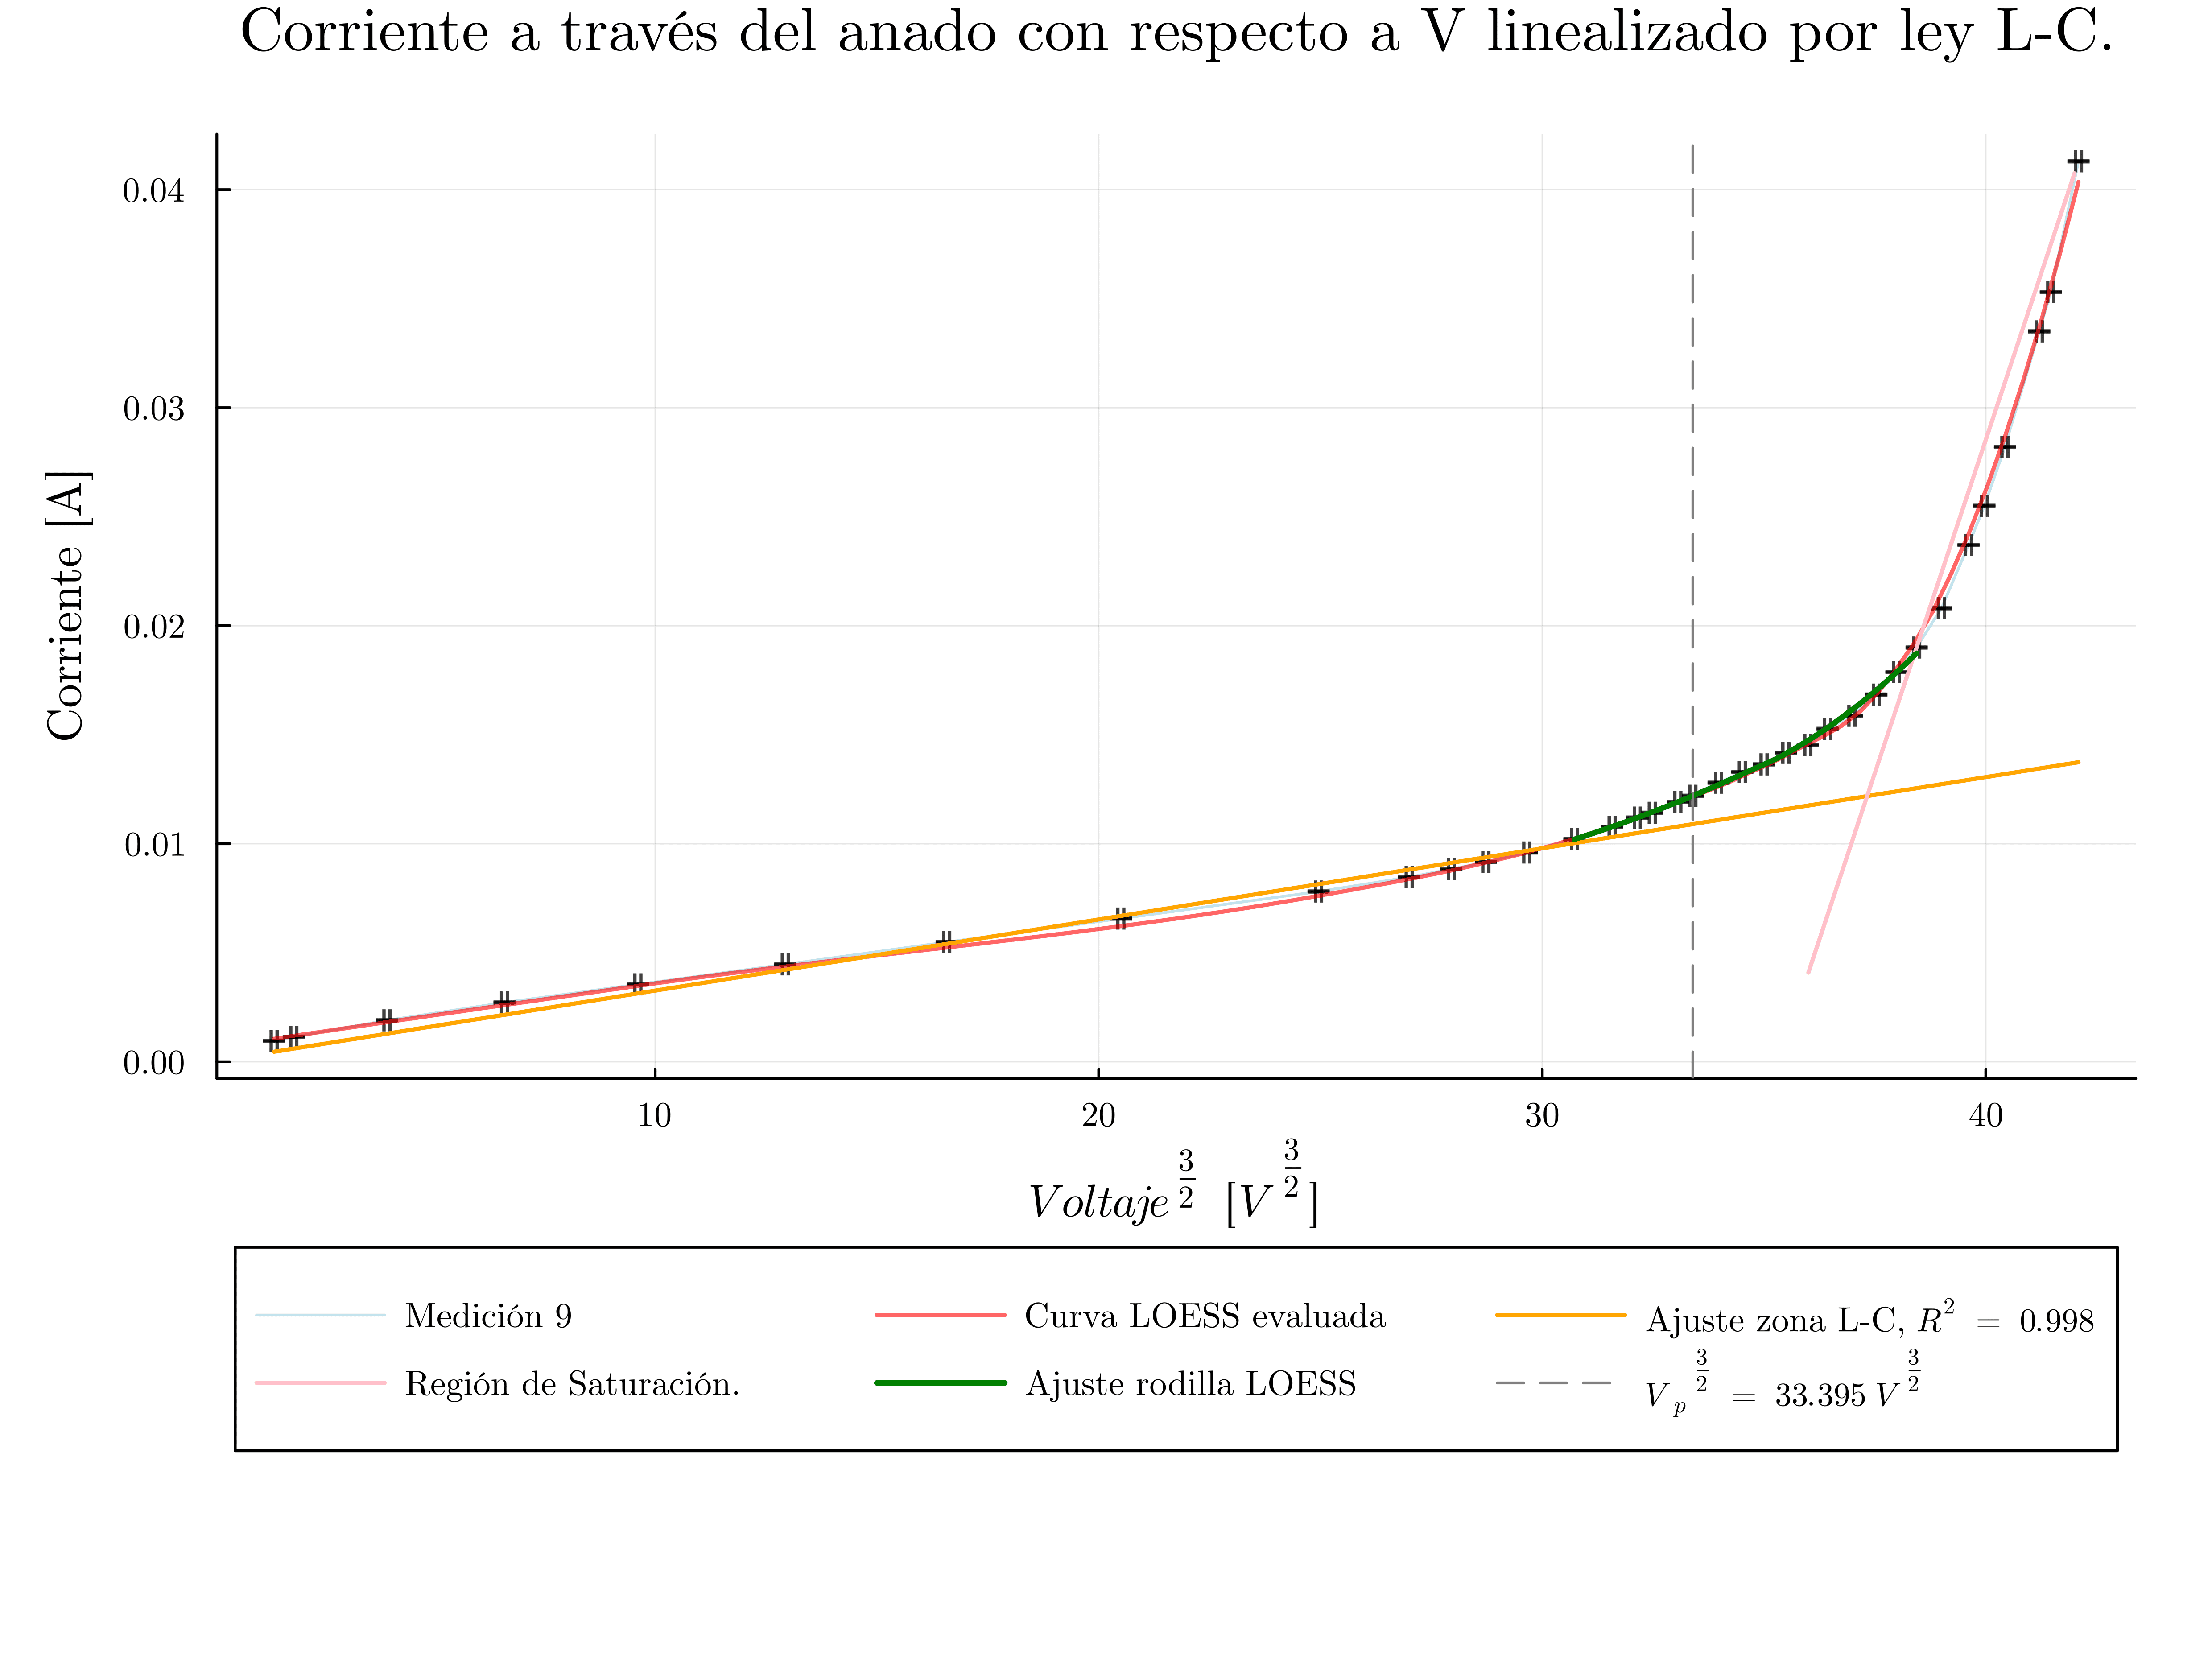
\includegraphics[width=\linewidth]{img/pot9.png}
		\caption{Barrido n°: 9}
		\label{fig:pot9}
	\end{subfigure}
	\hfill
	\begin{subfigure}[b]{0.49\textwidth}
		\centering
		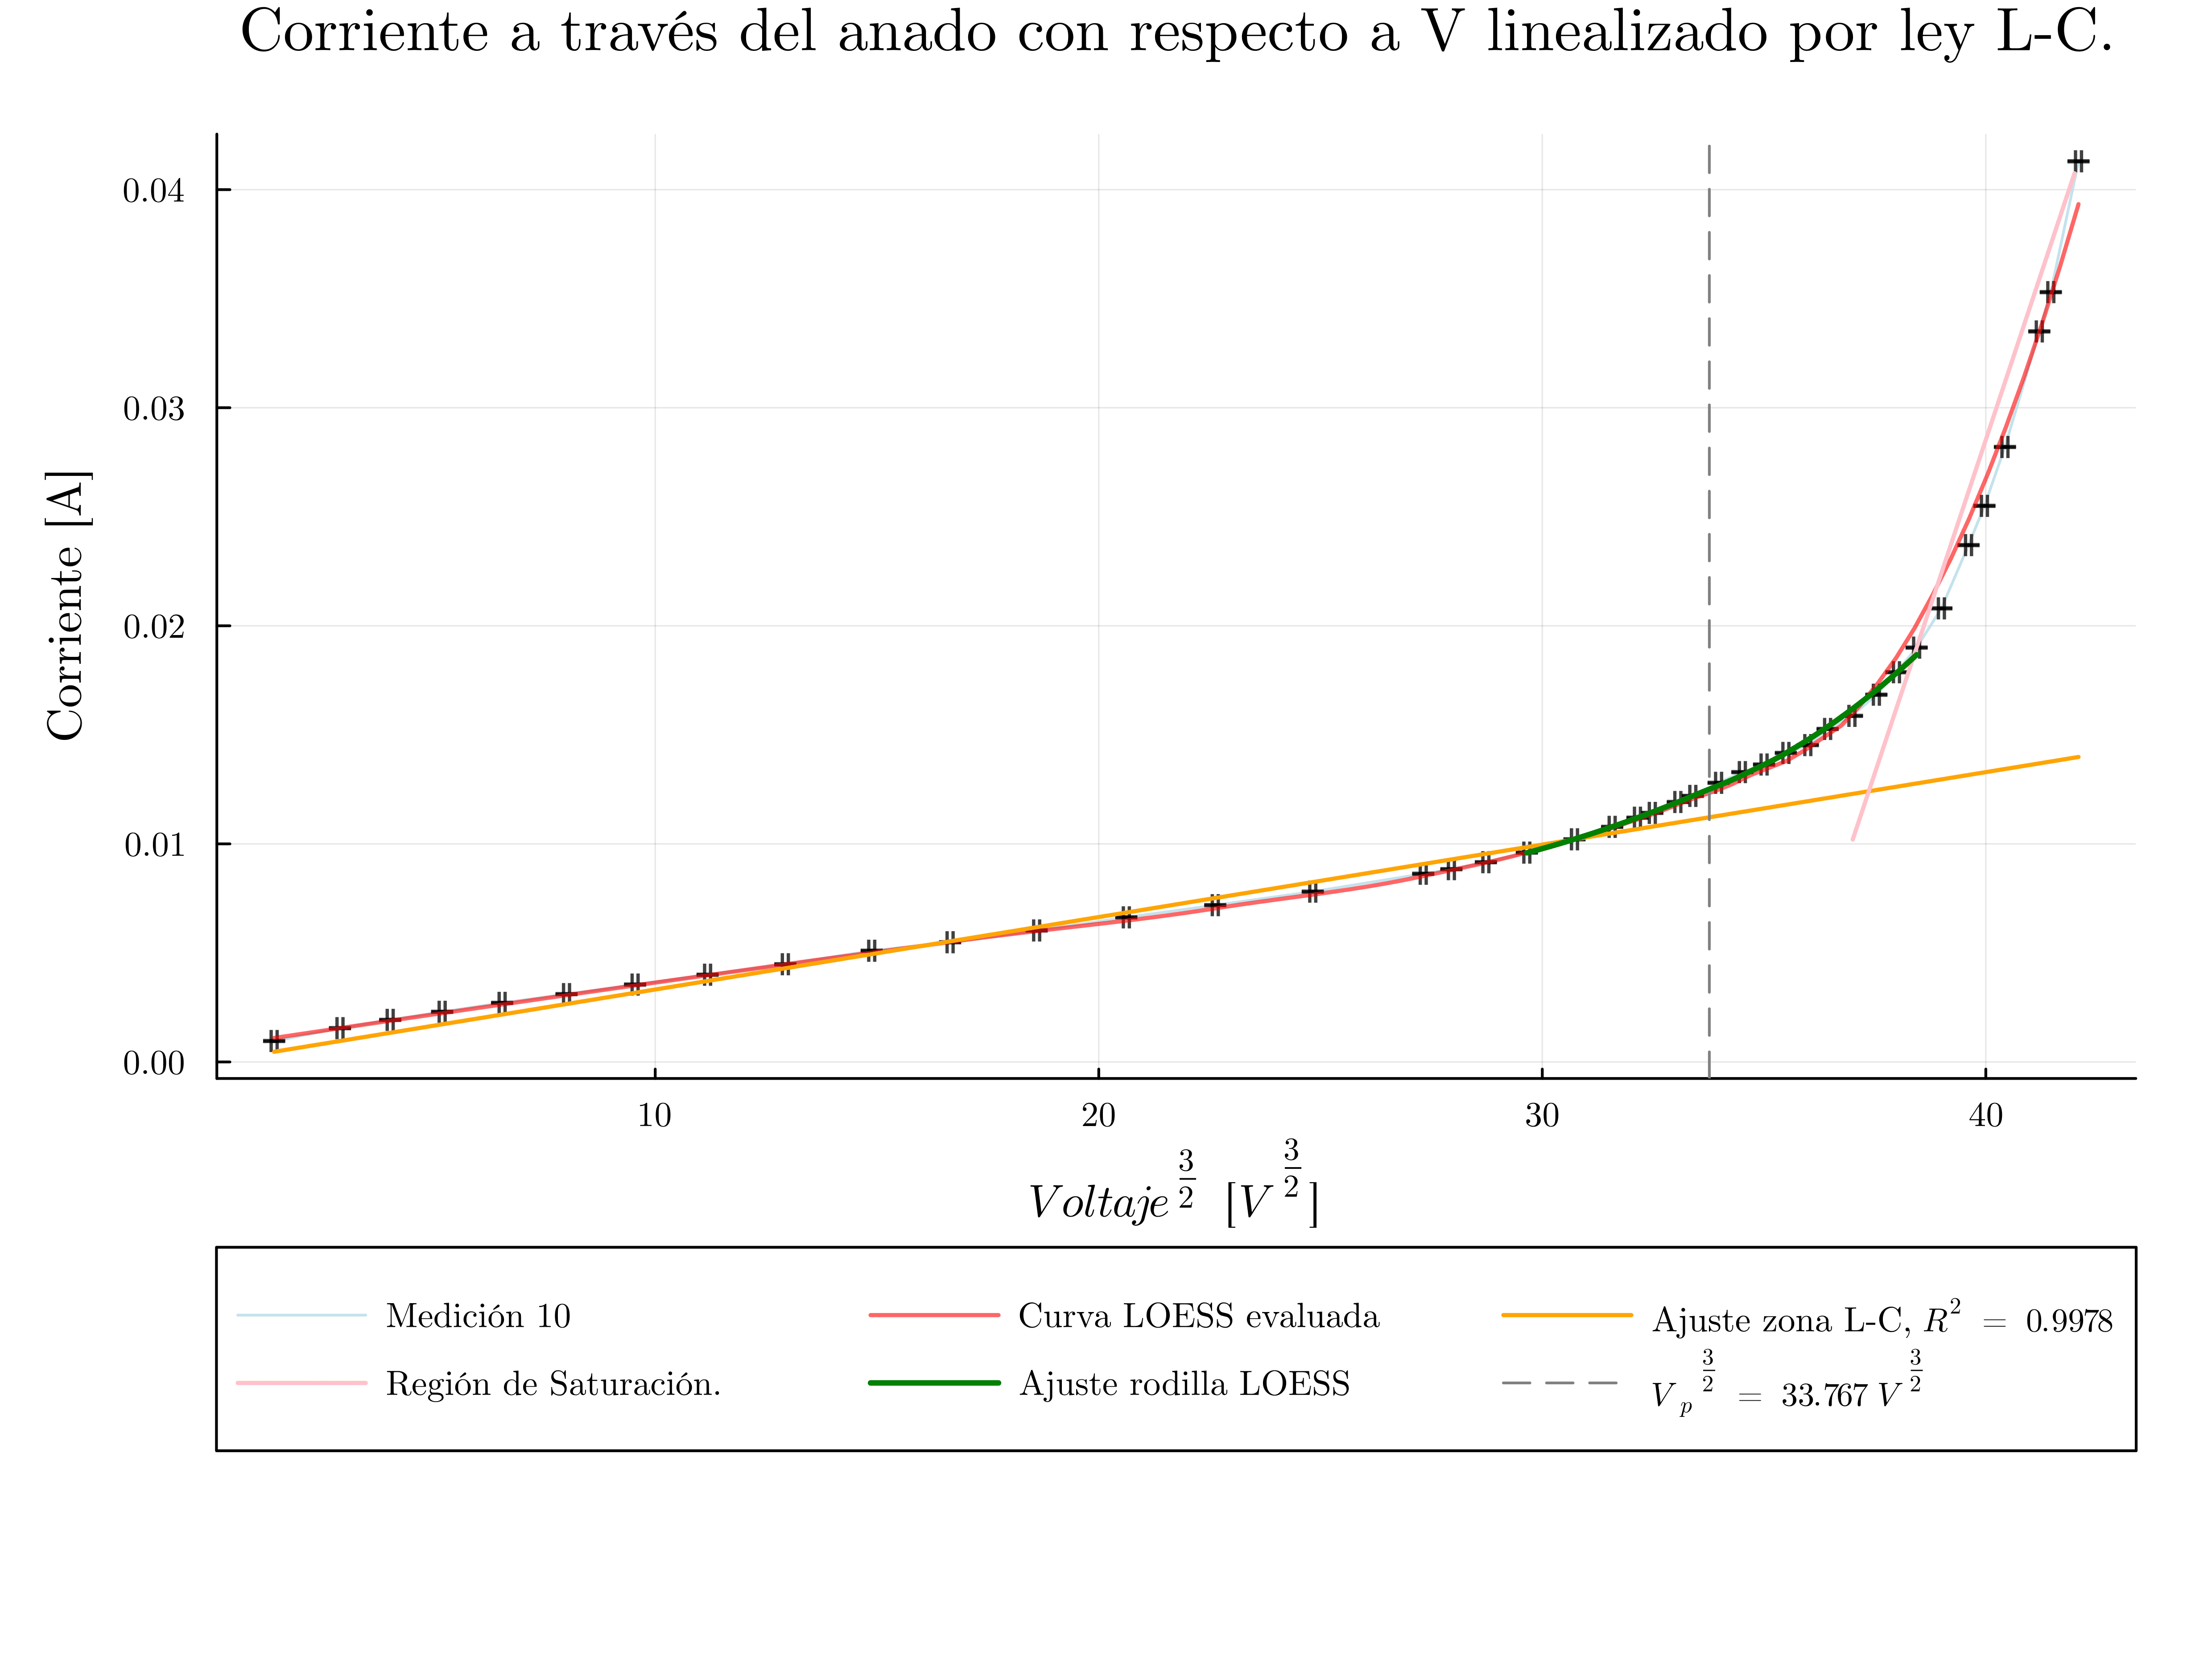
\includegraphics[width=\linewidth]{img/pot10.png}
		\caption{Barrido n°: 10}
		\label{fig:pot10}
	\end{subfigure}
	
	\caption{Corriente con respecto a $V^{\nicefrac{3}{2}}$, para los 10 barridos realizados, donde se puede apreciar el ajuste lineal junto con su coeficiente de $R^{2}$ realizado a la región regida por la ley de Child-Langmuir la cual presenta un comportamiento lineal. A su vez se muestran las curvas realizadas por LOESS, así como la recta de saturación y el punto de inflexión calculado mediante derivación numérica.}
	\label{fig:pots}
\end{figure}

\twocolumngrid



% Please add the following required packages to your document preamble:
% \usepackage{graphicx}
\begin{table}[H]
	\centering
	\resizebox{\columnwidth}{!}{%
		\begin{tabular}{|c|c|c|c|c|}
			\hline
			$Vp^{\nicefrac{3}{2}}\ [V^{\nicefrac{3}{2}}]$ & Vp $ [V]$ & limite inf $ [V]$ & limite sup $ [V]$ & Intv. de confiabilidad ($\pm\ [V]$) \\ \hline
			35.267          & 10.75     & 9.6               & 11.29             & 0.845                       \\ \hline
			35.334          & 10.77     & 9.4               & 11.16             & 0.88                        \\ \hline
			34.661          & 10.63     & 9.61              & 11.17             & 0.78                        \\ \hline
			34.464          & 10.59     & 9.6               & 11.16             & 0.78                        \\ \hline
			34.211          & 10.54     & 9.59              & 11.16             & 0.785                       \\ \hline
			33.875          & 10.47     & 9.65              & 11.18             & 0.765                       \\ \hline
			35.29           & 10.76     & 9.61              & 11.18             & 0.785                       \\ \hline
			34.195          & 10.54     & 9.59              & 11.18             & 0.795                       \\ \hline
			33.395          & 10.37     & 9.58              & 11.17             & 0.795                       \\ \hline
			33.767          & 10.45     & 9.58              & 11.18             & 0.8                         \\ \hline
		\end{tabular}%
	}
	\caption{ Puntos de inflexión asociados al potencial de de ionización encontrados mediante criterio de la tercer derivada, y derivación numérica, a la par se muestran los limites de confiabilidad inferiores obtenidos de la interacción de la recta de ajuste de la ley de Child-Langmuir con la curva de todo el barrido generada por LOESS; los limites superiores, obtenidos mediante la recta ajuste de la ley de Child-Langmuir,  con la recta de la región de saturación. Finalmente se muestra el valor del intervalo de confiabilidad obtenido mediante el promedio de la distancia de $Vp$ a los limites.}
	\label{tab:pots}
\end{table}


Se obtuvo un valor de energía de ionización promedio de $V_{p}\ =\ 	10.59\ eV,\ \sigma\ =\ 0.140\ eV$, con un intervalo de confianza promedio de $0.8 eV$; el cual se aproxima con un error porcentual $1.54\ \%$ al potencial de ionización de mercurio \cite{lide}, cuyos vapor es utilizado en el diseño de tiratrones. Las figuras \ut{\ref{fig:potderps1} - \ref{fig:potderps10}} en el apéndice \ut{A}, y \ut{\ref{fig:potderst1} - \ref{fig:potderst10}}   muestran la primera derivada con segunda derivada,  y tercer derivada respectivamente  para cada una de la regiones denominadas como \textit{Ajuste rodilla LOESS} para las figuras, \ut{\ref{fig:pot1} - \ref{fig:pot10}}, en ellas se puede apreciar que a pesar de que todos los puntos en esta región fueron utilizados para realizar el ajuste por método de LOESS, debido a la presencia de ruido en las mediciones esta curva presenta varios puntos de inflexiones como consecuencia de buscar una curva suave. Debido a esto se pueden apreciar cuatro puntos donde la tercer derivada es visiblemente diferente de cero, no obstante los puntos del dominio de la tercer derivada asociados a esos valores no son iguales a cero, lo que implica que existen puntos entre la distancia de la equipartición que cumplen el criterio de la tercer derivada, no obstante debido a que la distancia de la equipartición es del tamaño de la mínima escala del multímetro, no es valido refinar la equipartición. Por consiguiente se estableció un intervalo de confiabilidad en donde se encontraría el potencial de ionización en caso de repetirse con otra serie de datos. Así mismo este error puede ser reducido si se utilizara una fuente de voltaje que permitiera realizar cambios de potencial equidistantes y precisos, como seria un potenciómetro digital en configuración de divisor de voltaje con un OP-AMP de baja deriva  en configuración de seguidor de voltaje, así mismo se puede utilizar un multimétro 

\onecolumngrid

% Primer bloque de figuras
\begin{figure}[H]
	\centering
	\begin{subfigure}[b]{0.49\textwidth}
		\centering
		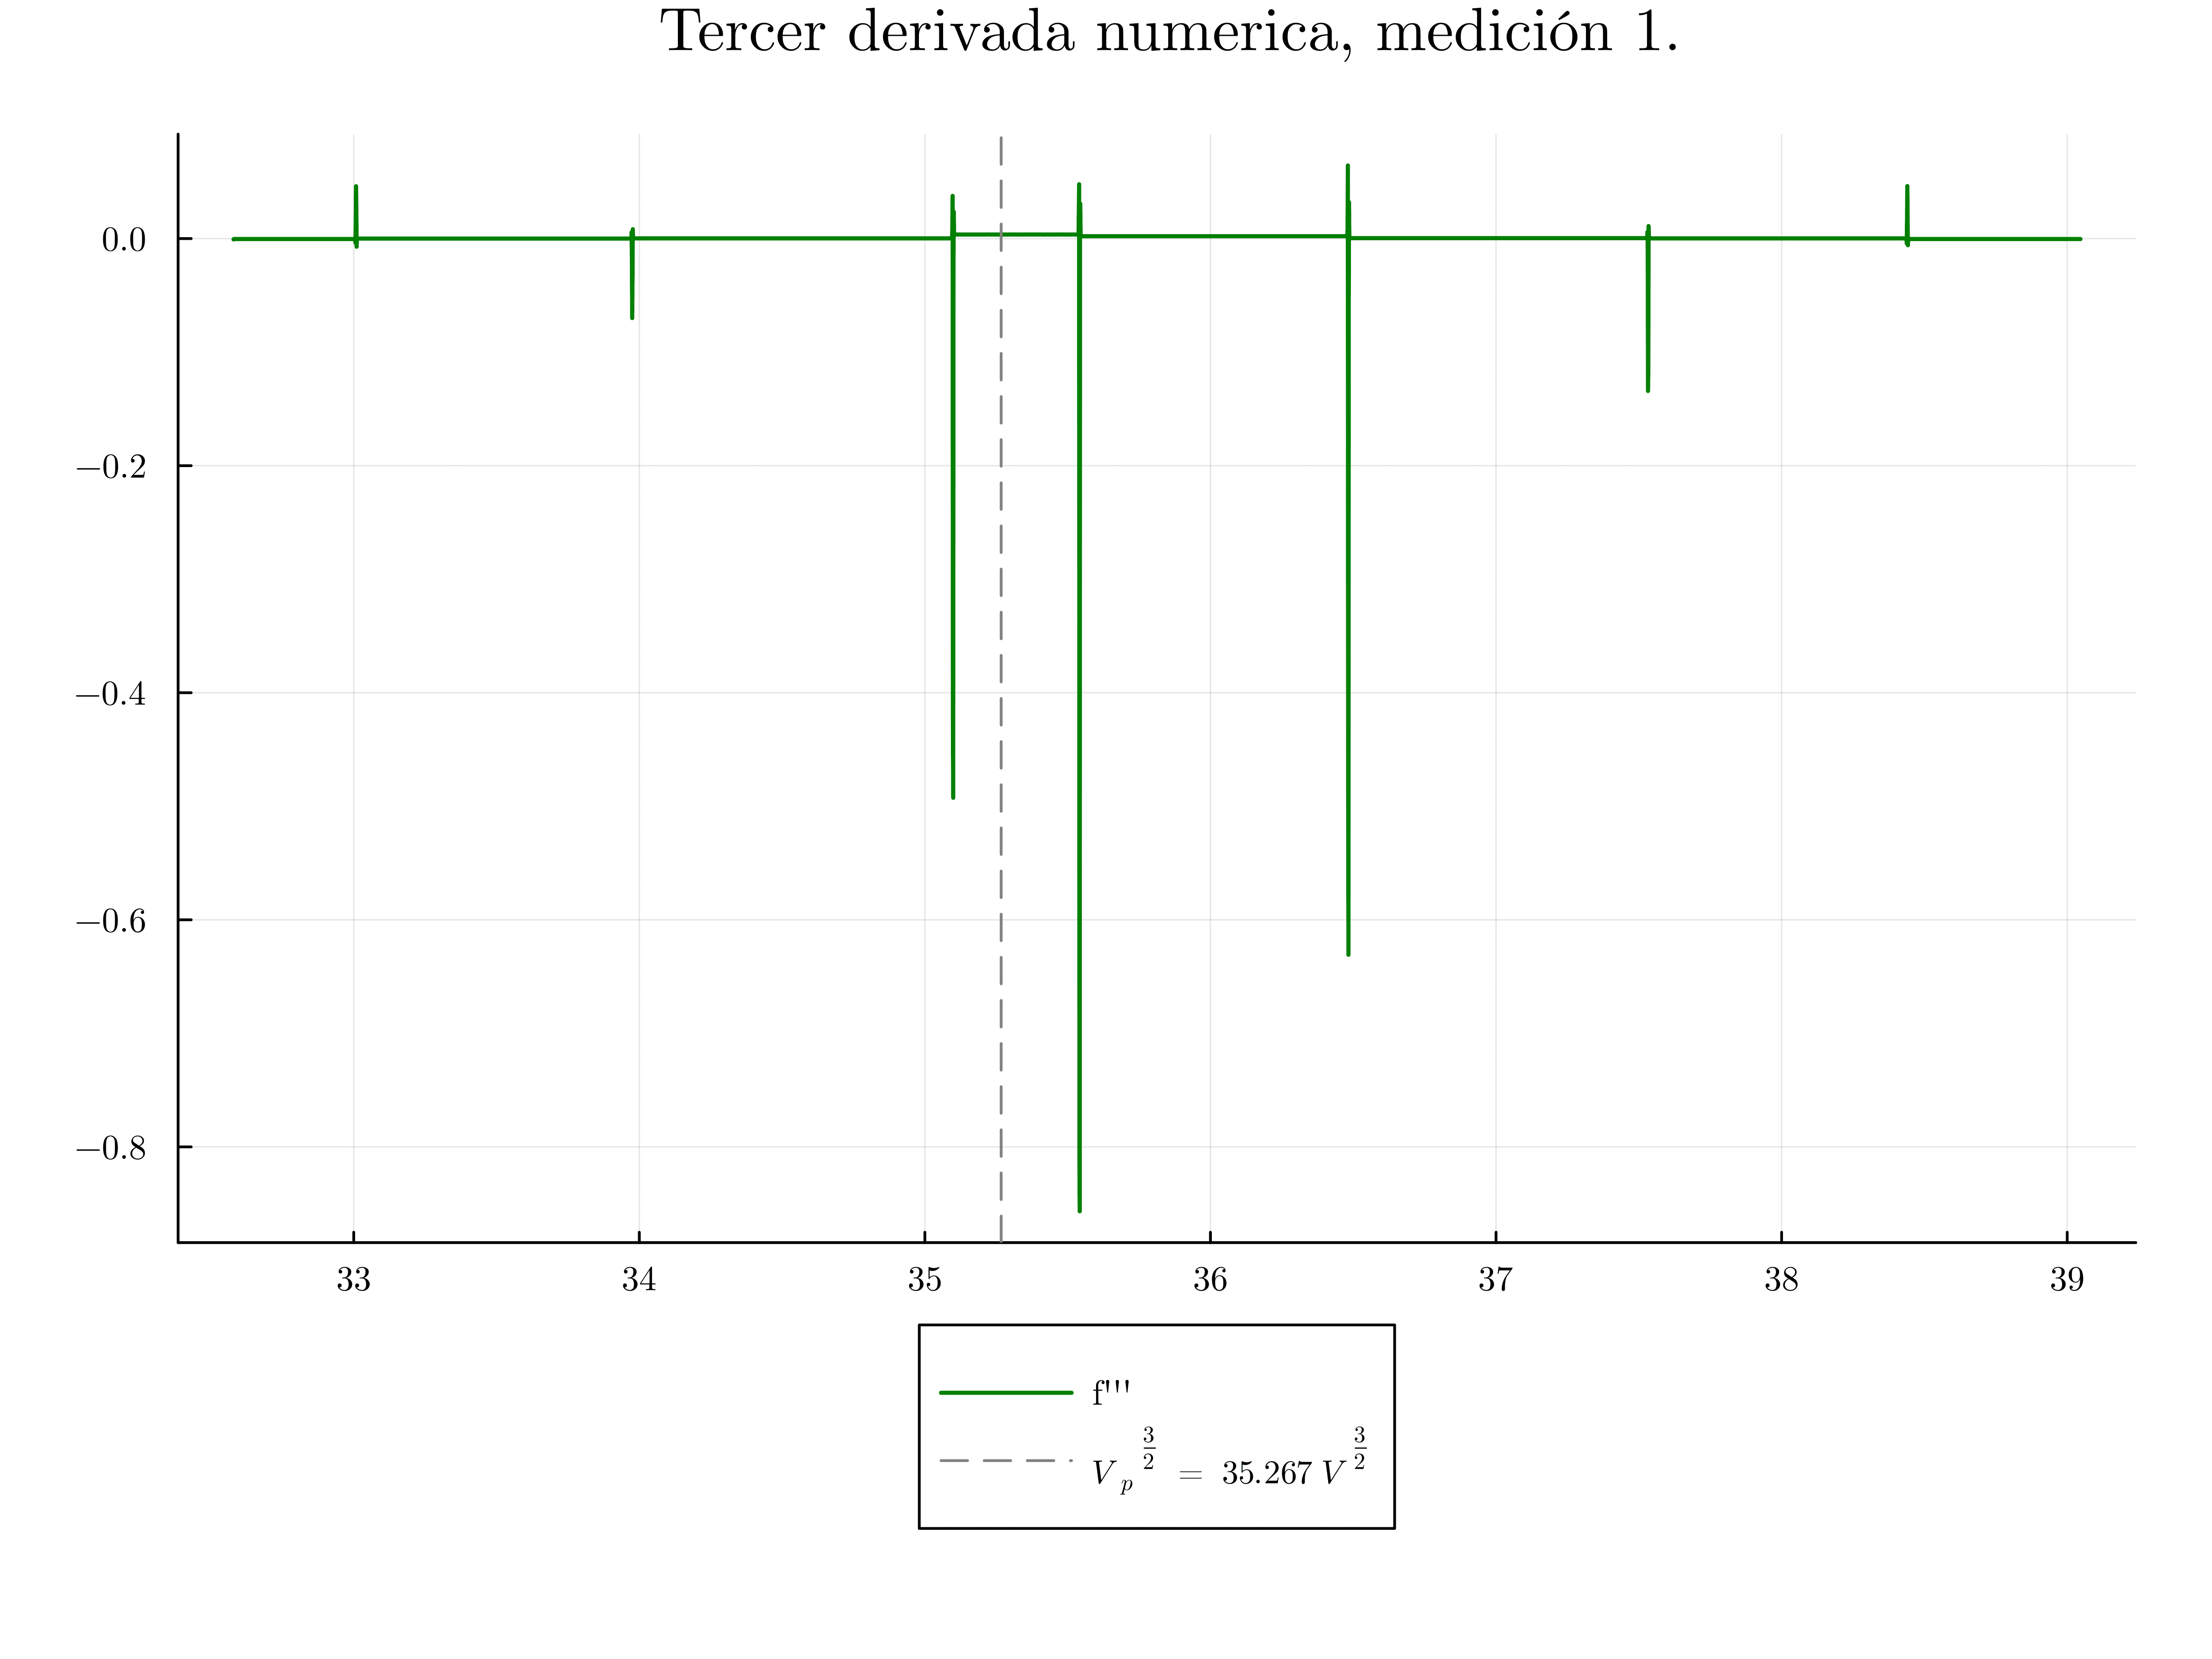
\includegraphics[width=\linewidth]{img/potderst1.png}
		\caption{Barrido n°: 1}
		\label{fig:potderst1}
	\end{subfigure}
	\hfill
	\begin{subfigure}[b]{0.49\textwidth}
		\centering
		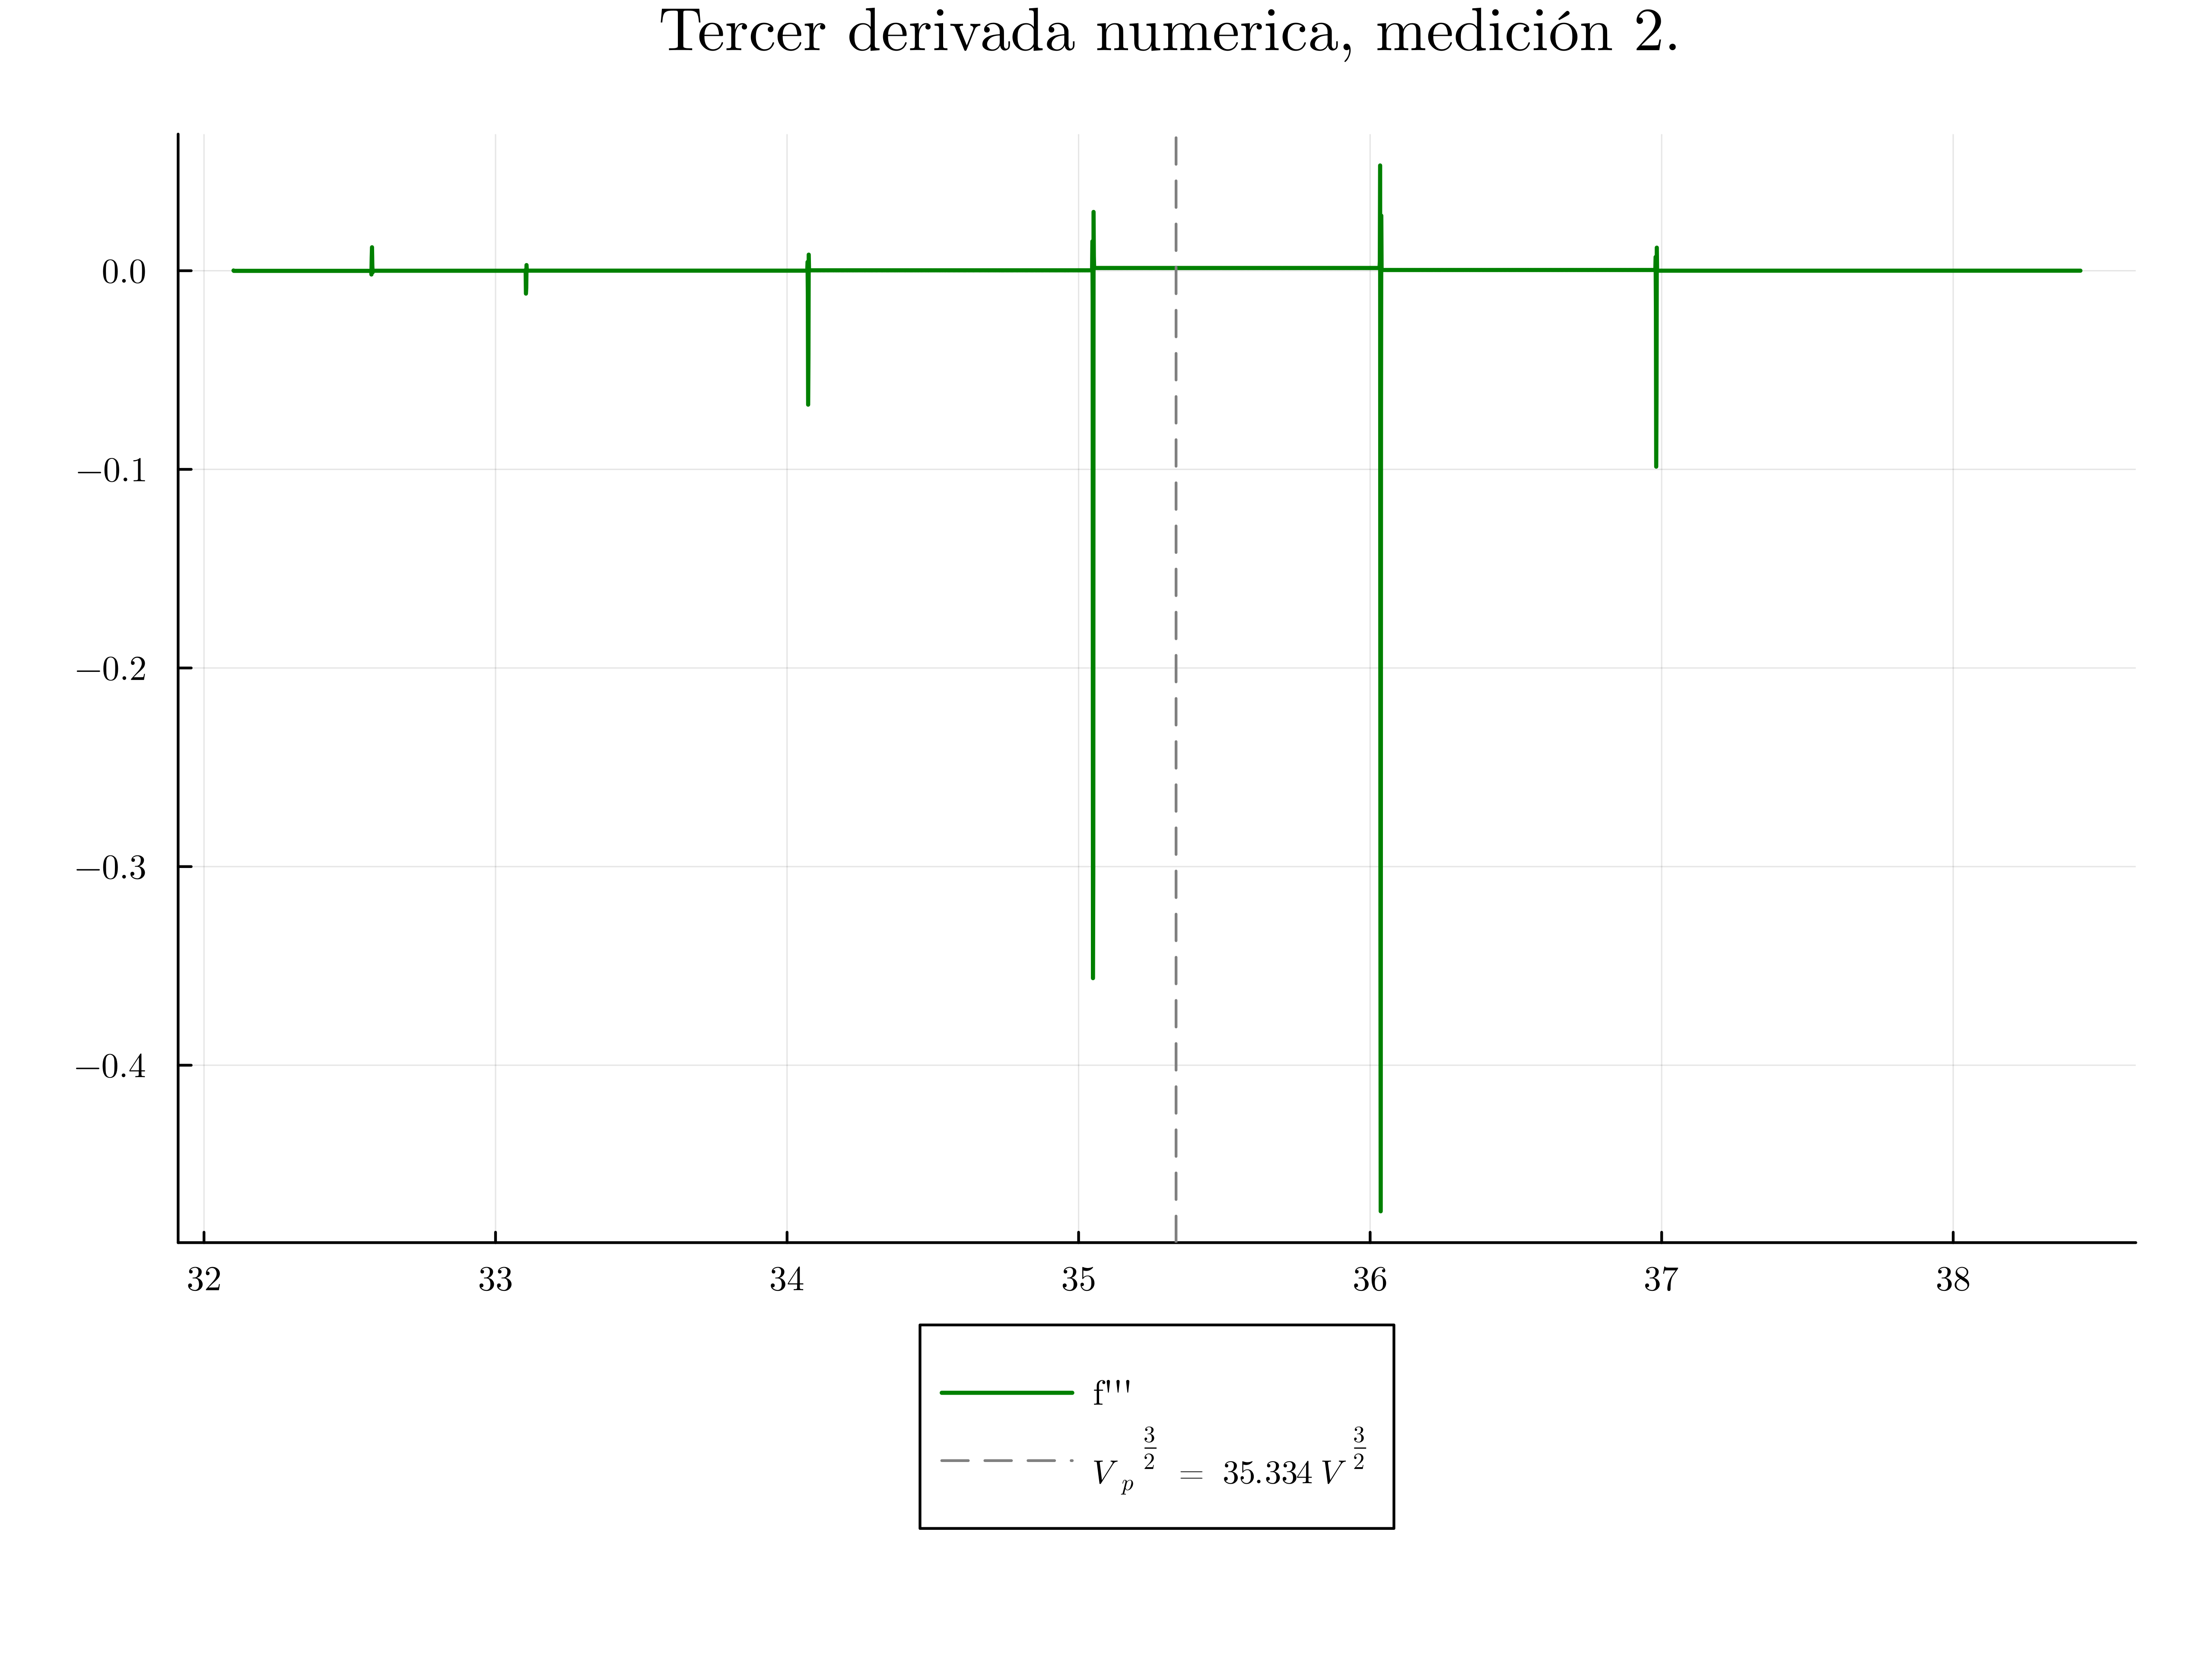
\includegraphics[width=\linewidth]{img/potderst2.png}
		\caption{Barrido n°: 2}
		\label{fig:potderst2}
	\end{subfigure}
	
\end{figure}

% segundo bloque de figuras
\begin{figure}[H]
	\ContinuedFloat
	\centering
	\begin{subfigure}[b]{0.49\textwidth}
		\centering
		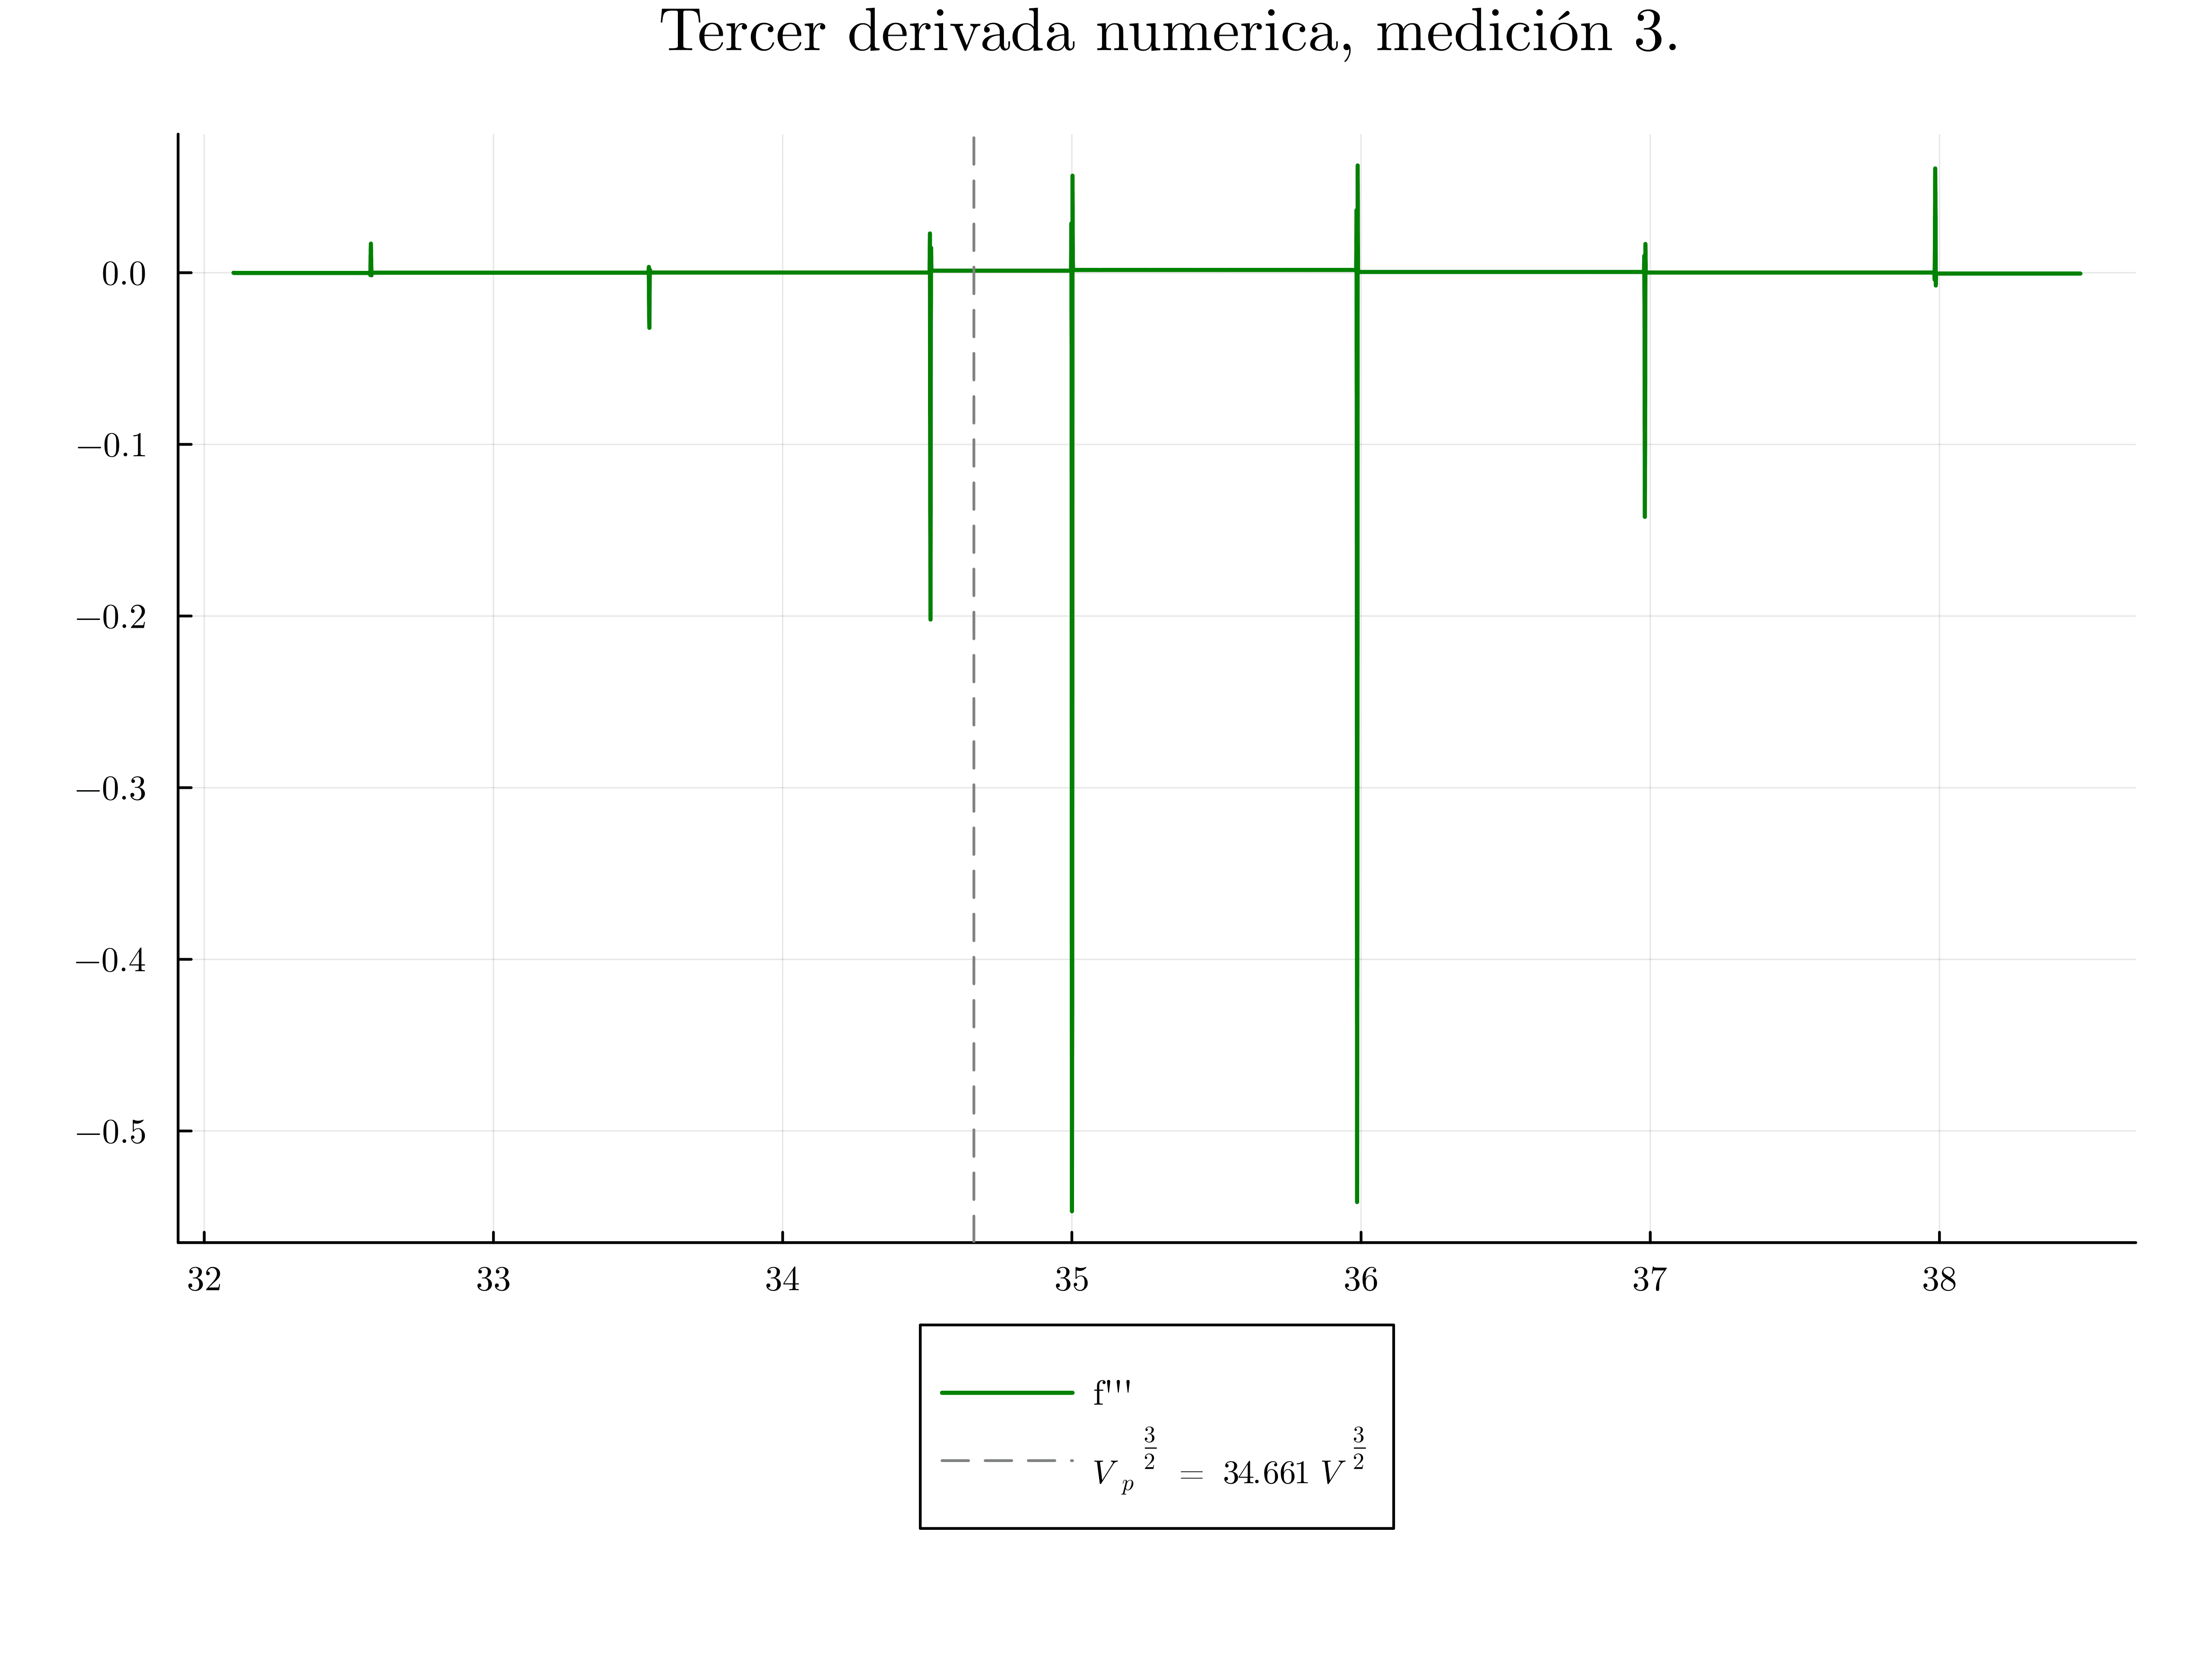
\includegraphics[width=\linewidth]{img/potderst3.png}
		\caption{Barrido n°: 3}
		\label{fig:potderst3}
	\end{subfigure}
	\hfill
	\begin{subfigure}[b]{0.49\textwidth}
		\centering
		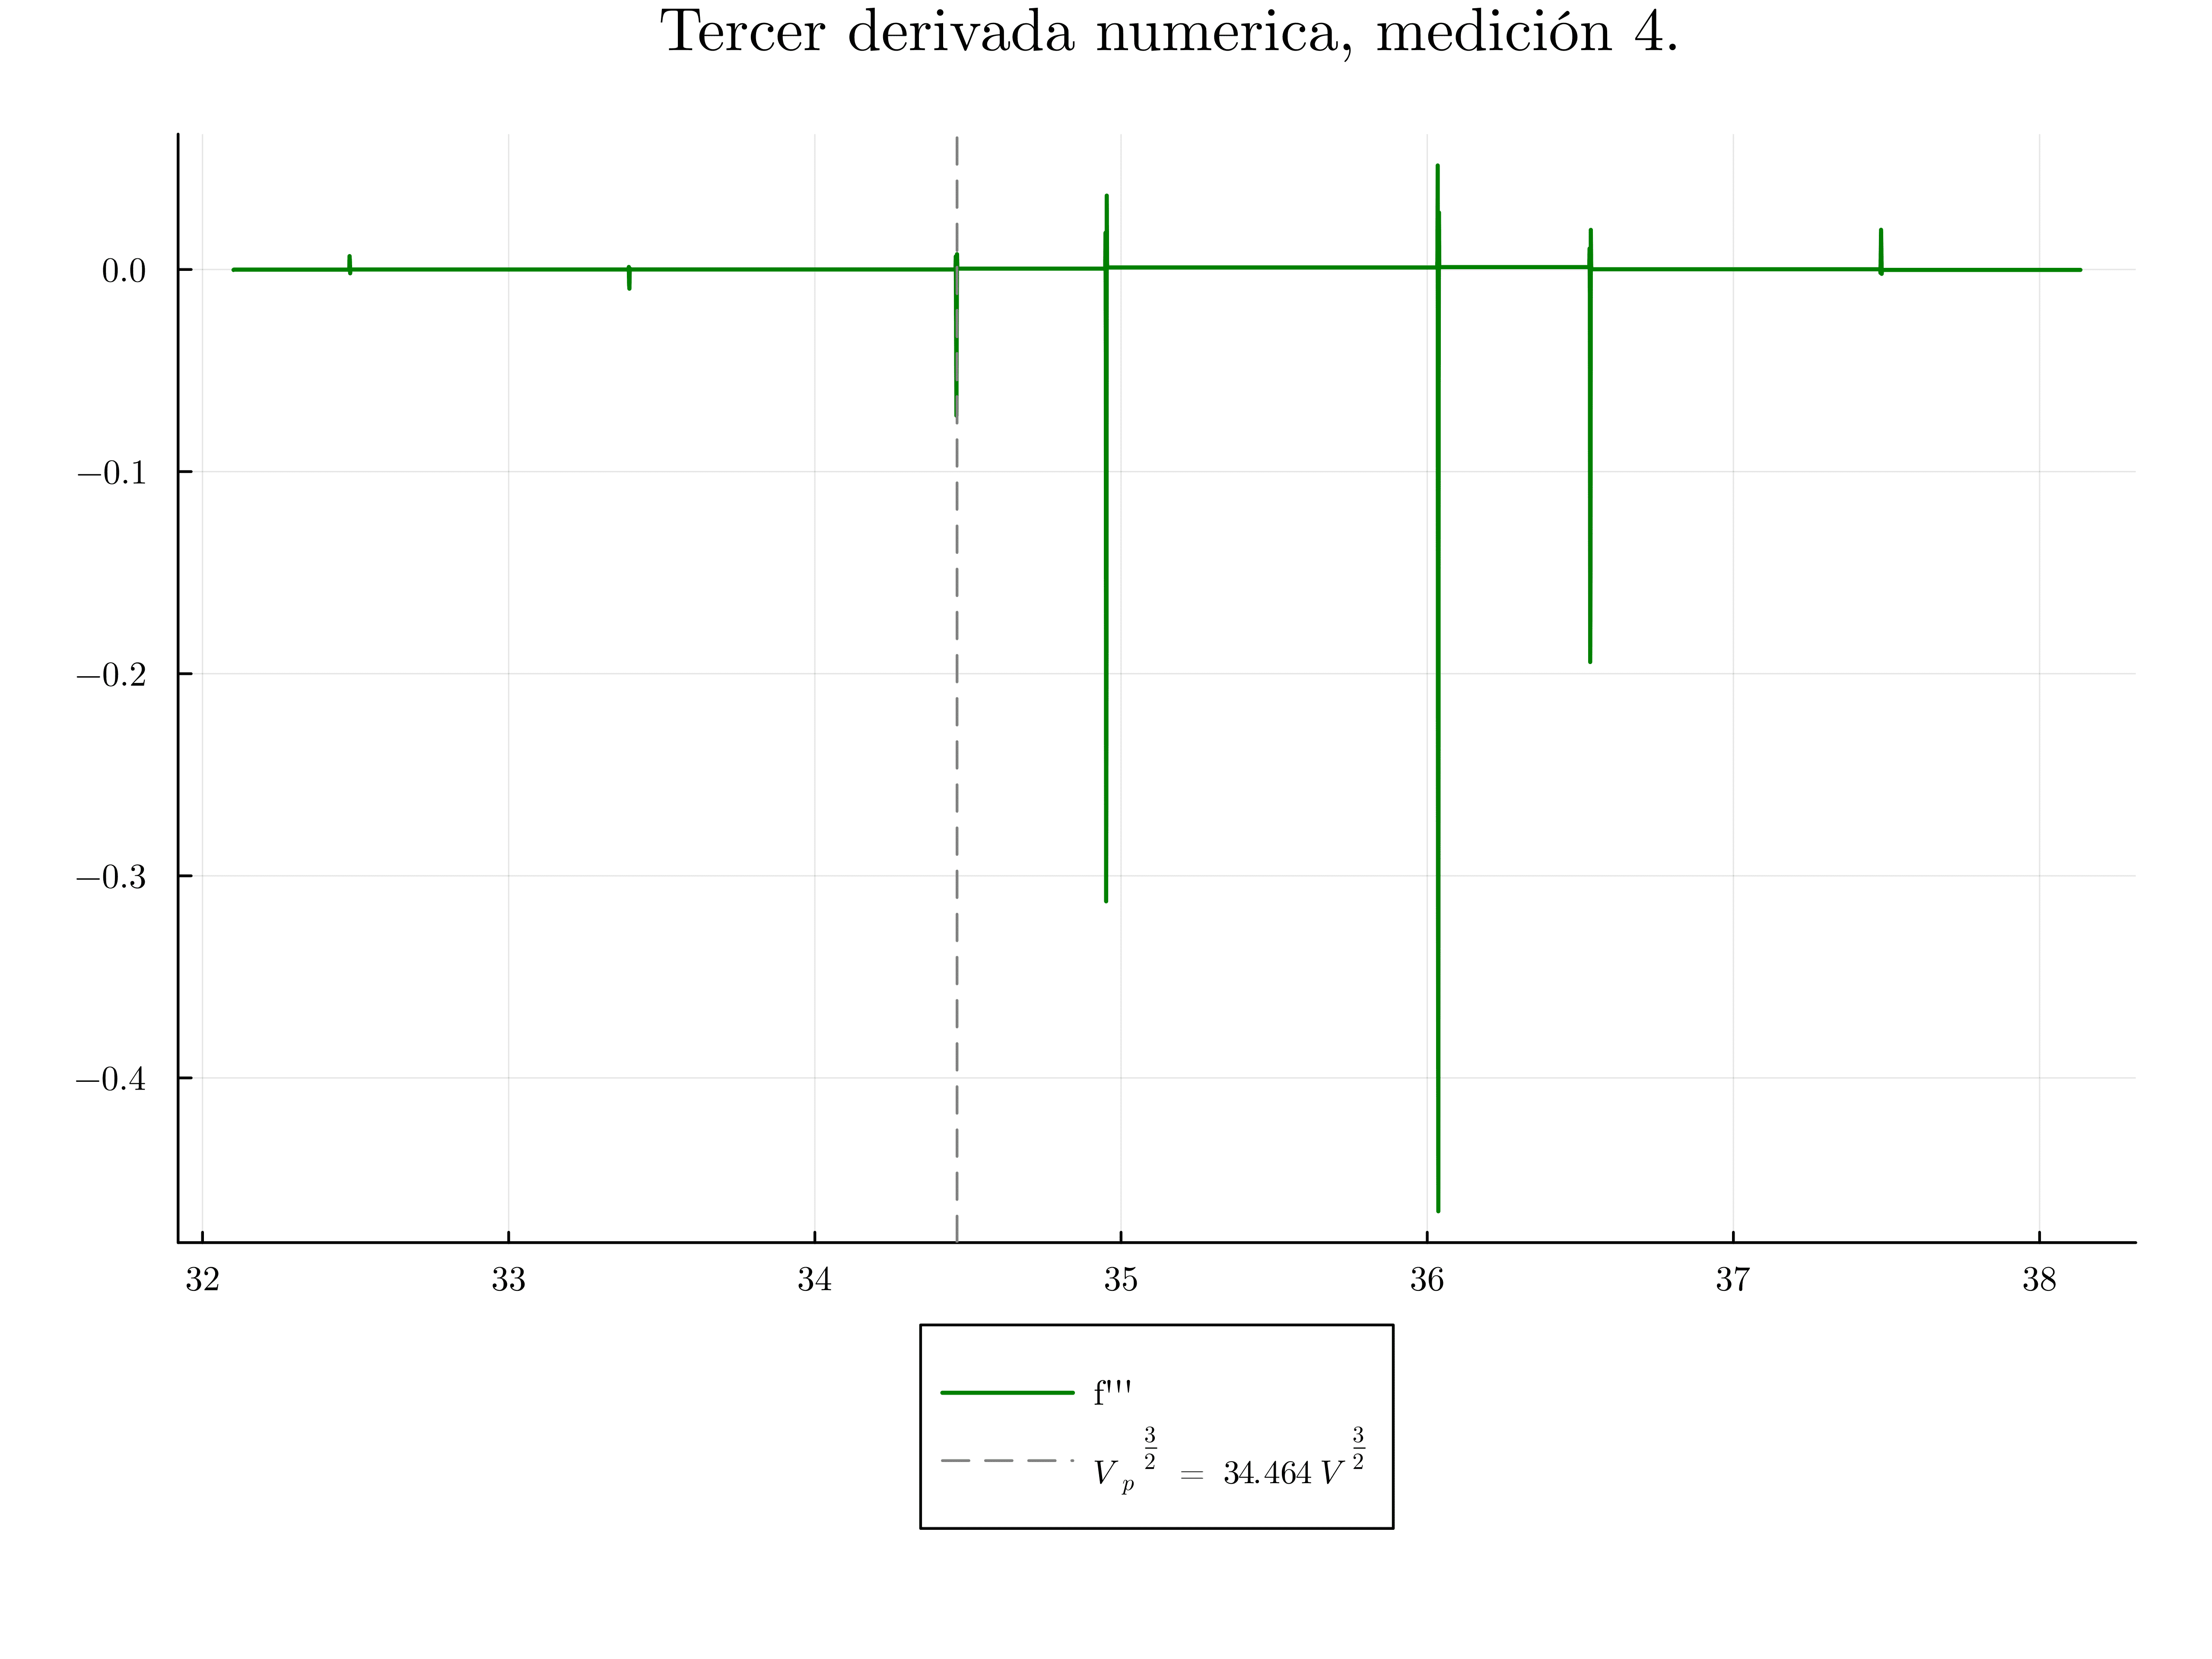
\includegraphics[width=\linewidth]{img/potderst4.png}
		\caption{Barrido n°: 4}
		\label{fig:potderst4}
	\end{subfigure}
	
\end{figure}

% teercer bloque de figuras
\begin{figure}[H]
	\ContinuedFloat % Indica que esta figura continúa de la anterior
	\centering
	\begin{subfigure}[b]{0.49\textwidth}
		\centering
		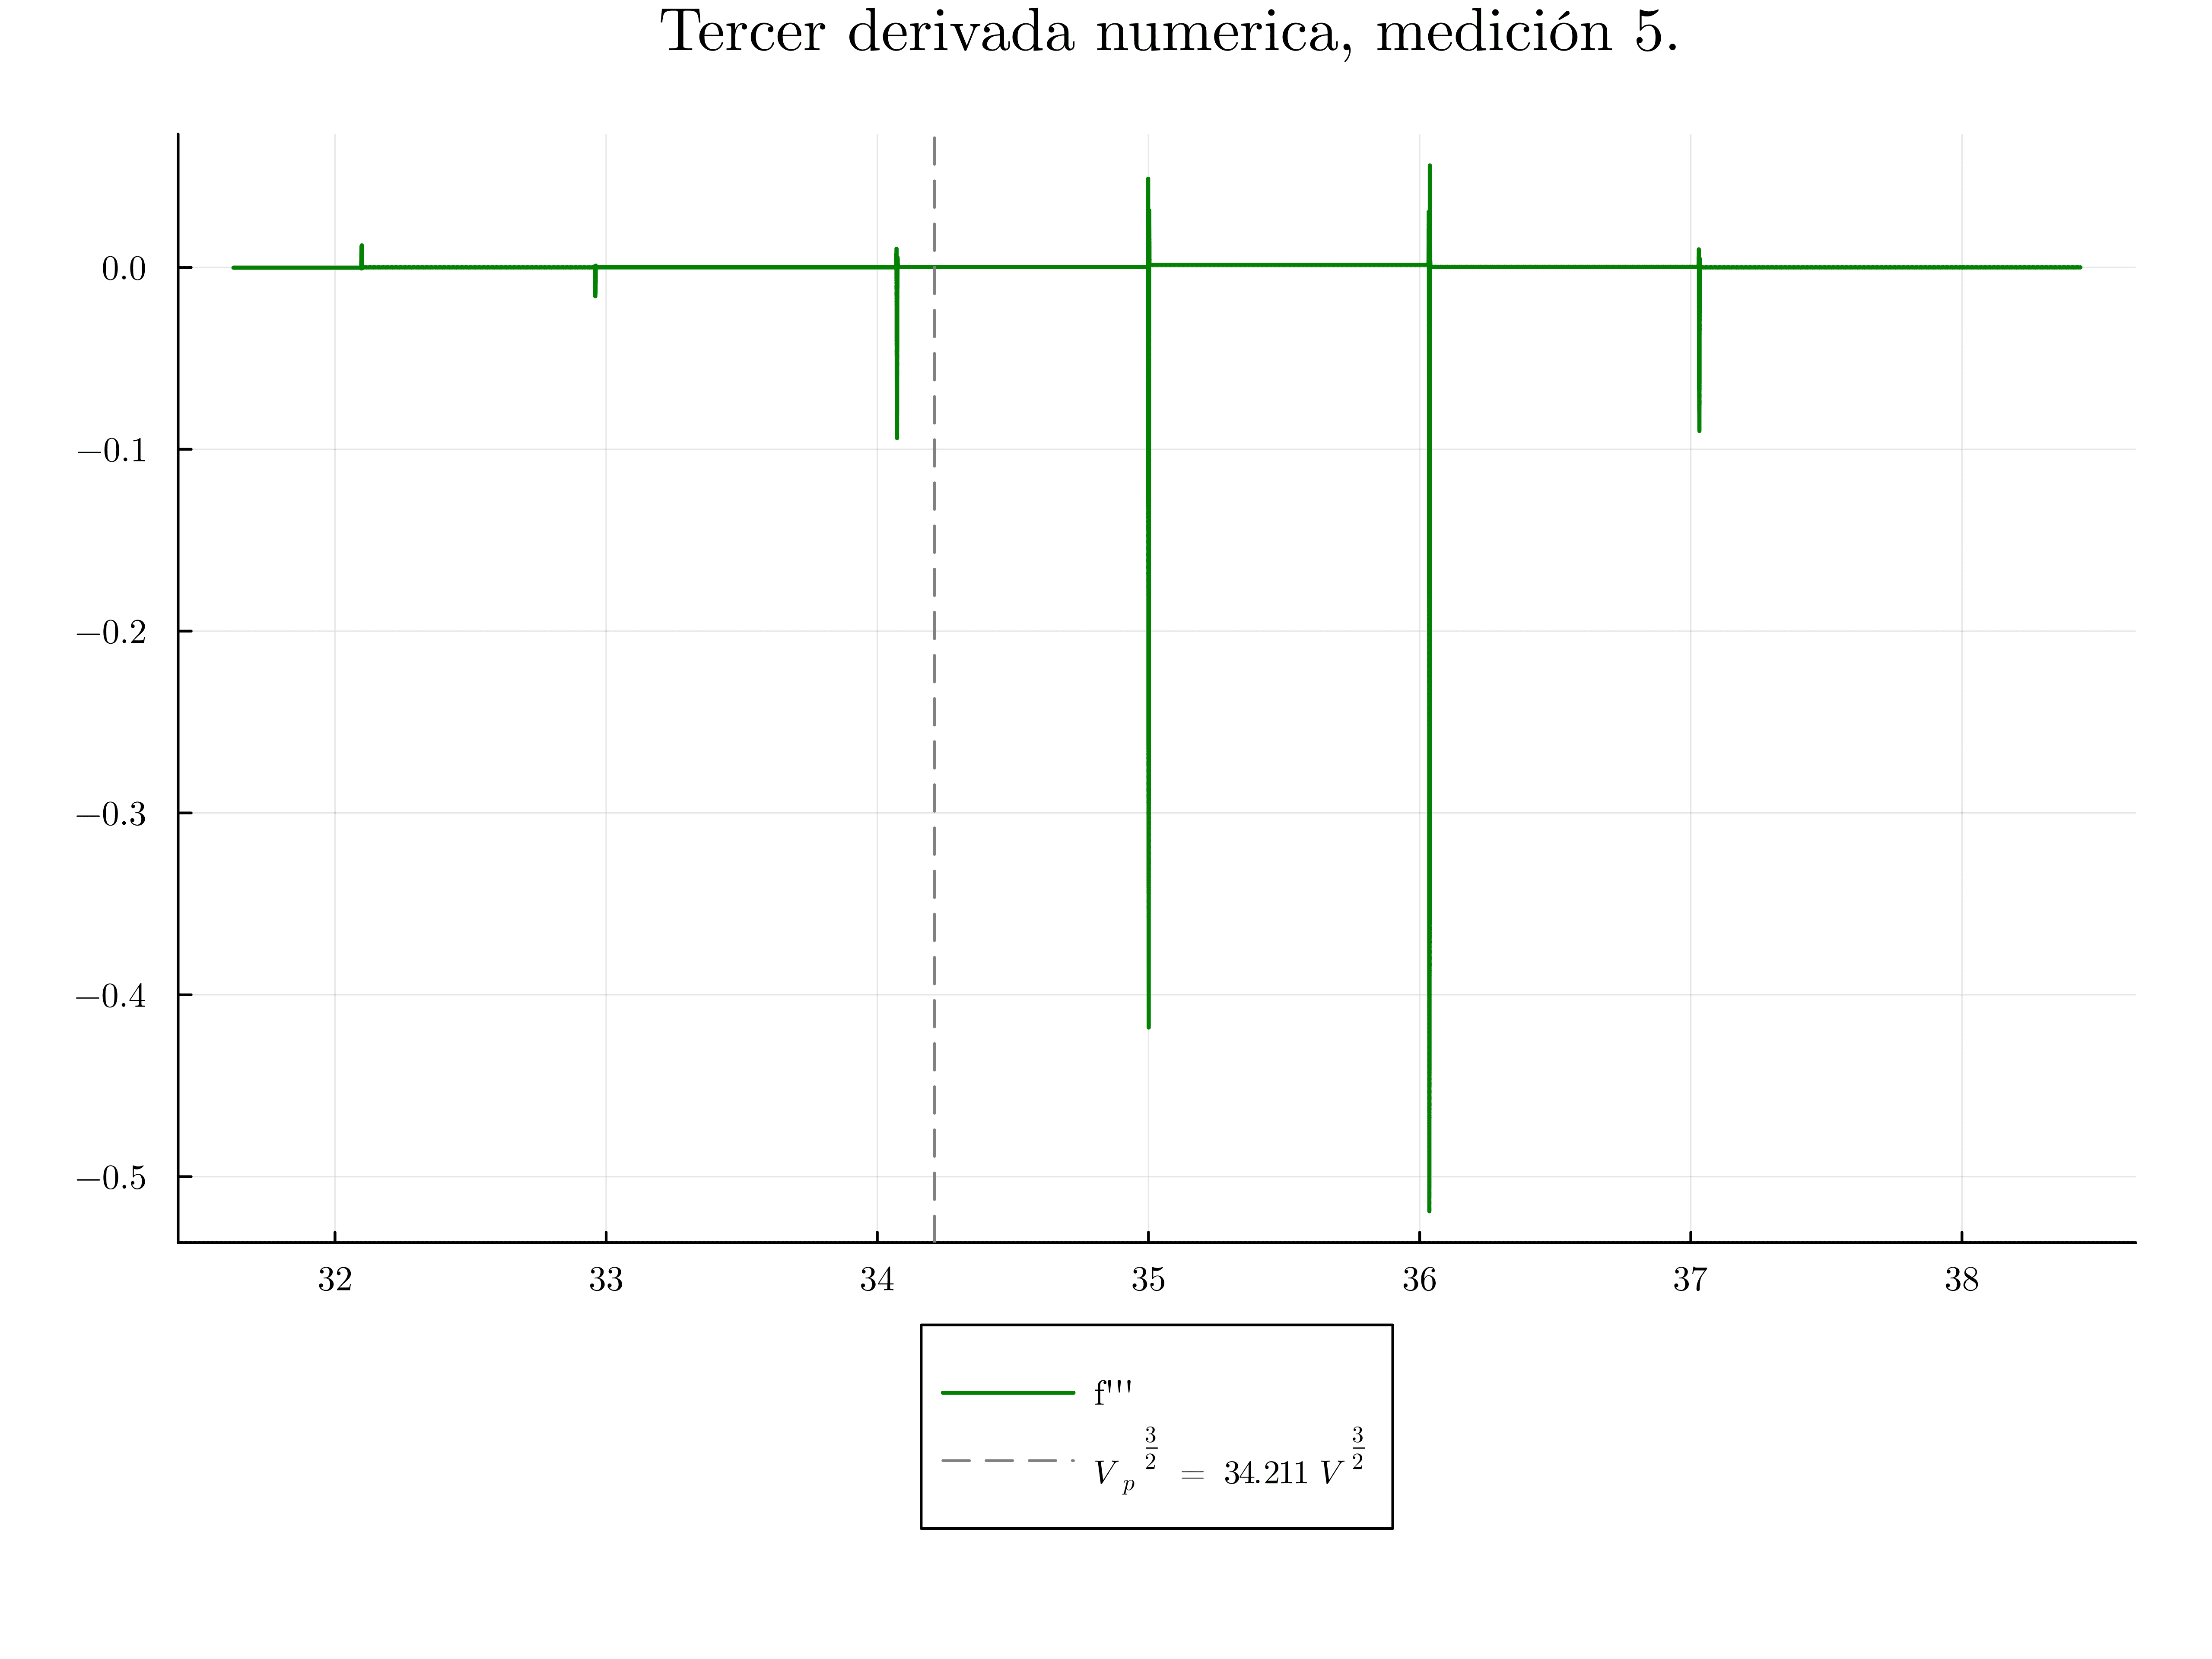
\includegraphics[width=\linewidth]{img/potderst5.png}
		\caption{Barrido n°: 5}
		\label{fig:potderst5}
	\end{subfigure}
	\hfill
	\begin{subfigure}[b]{0.49\textwidth}
		\centering
		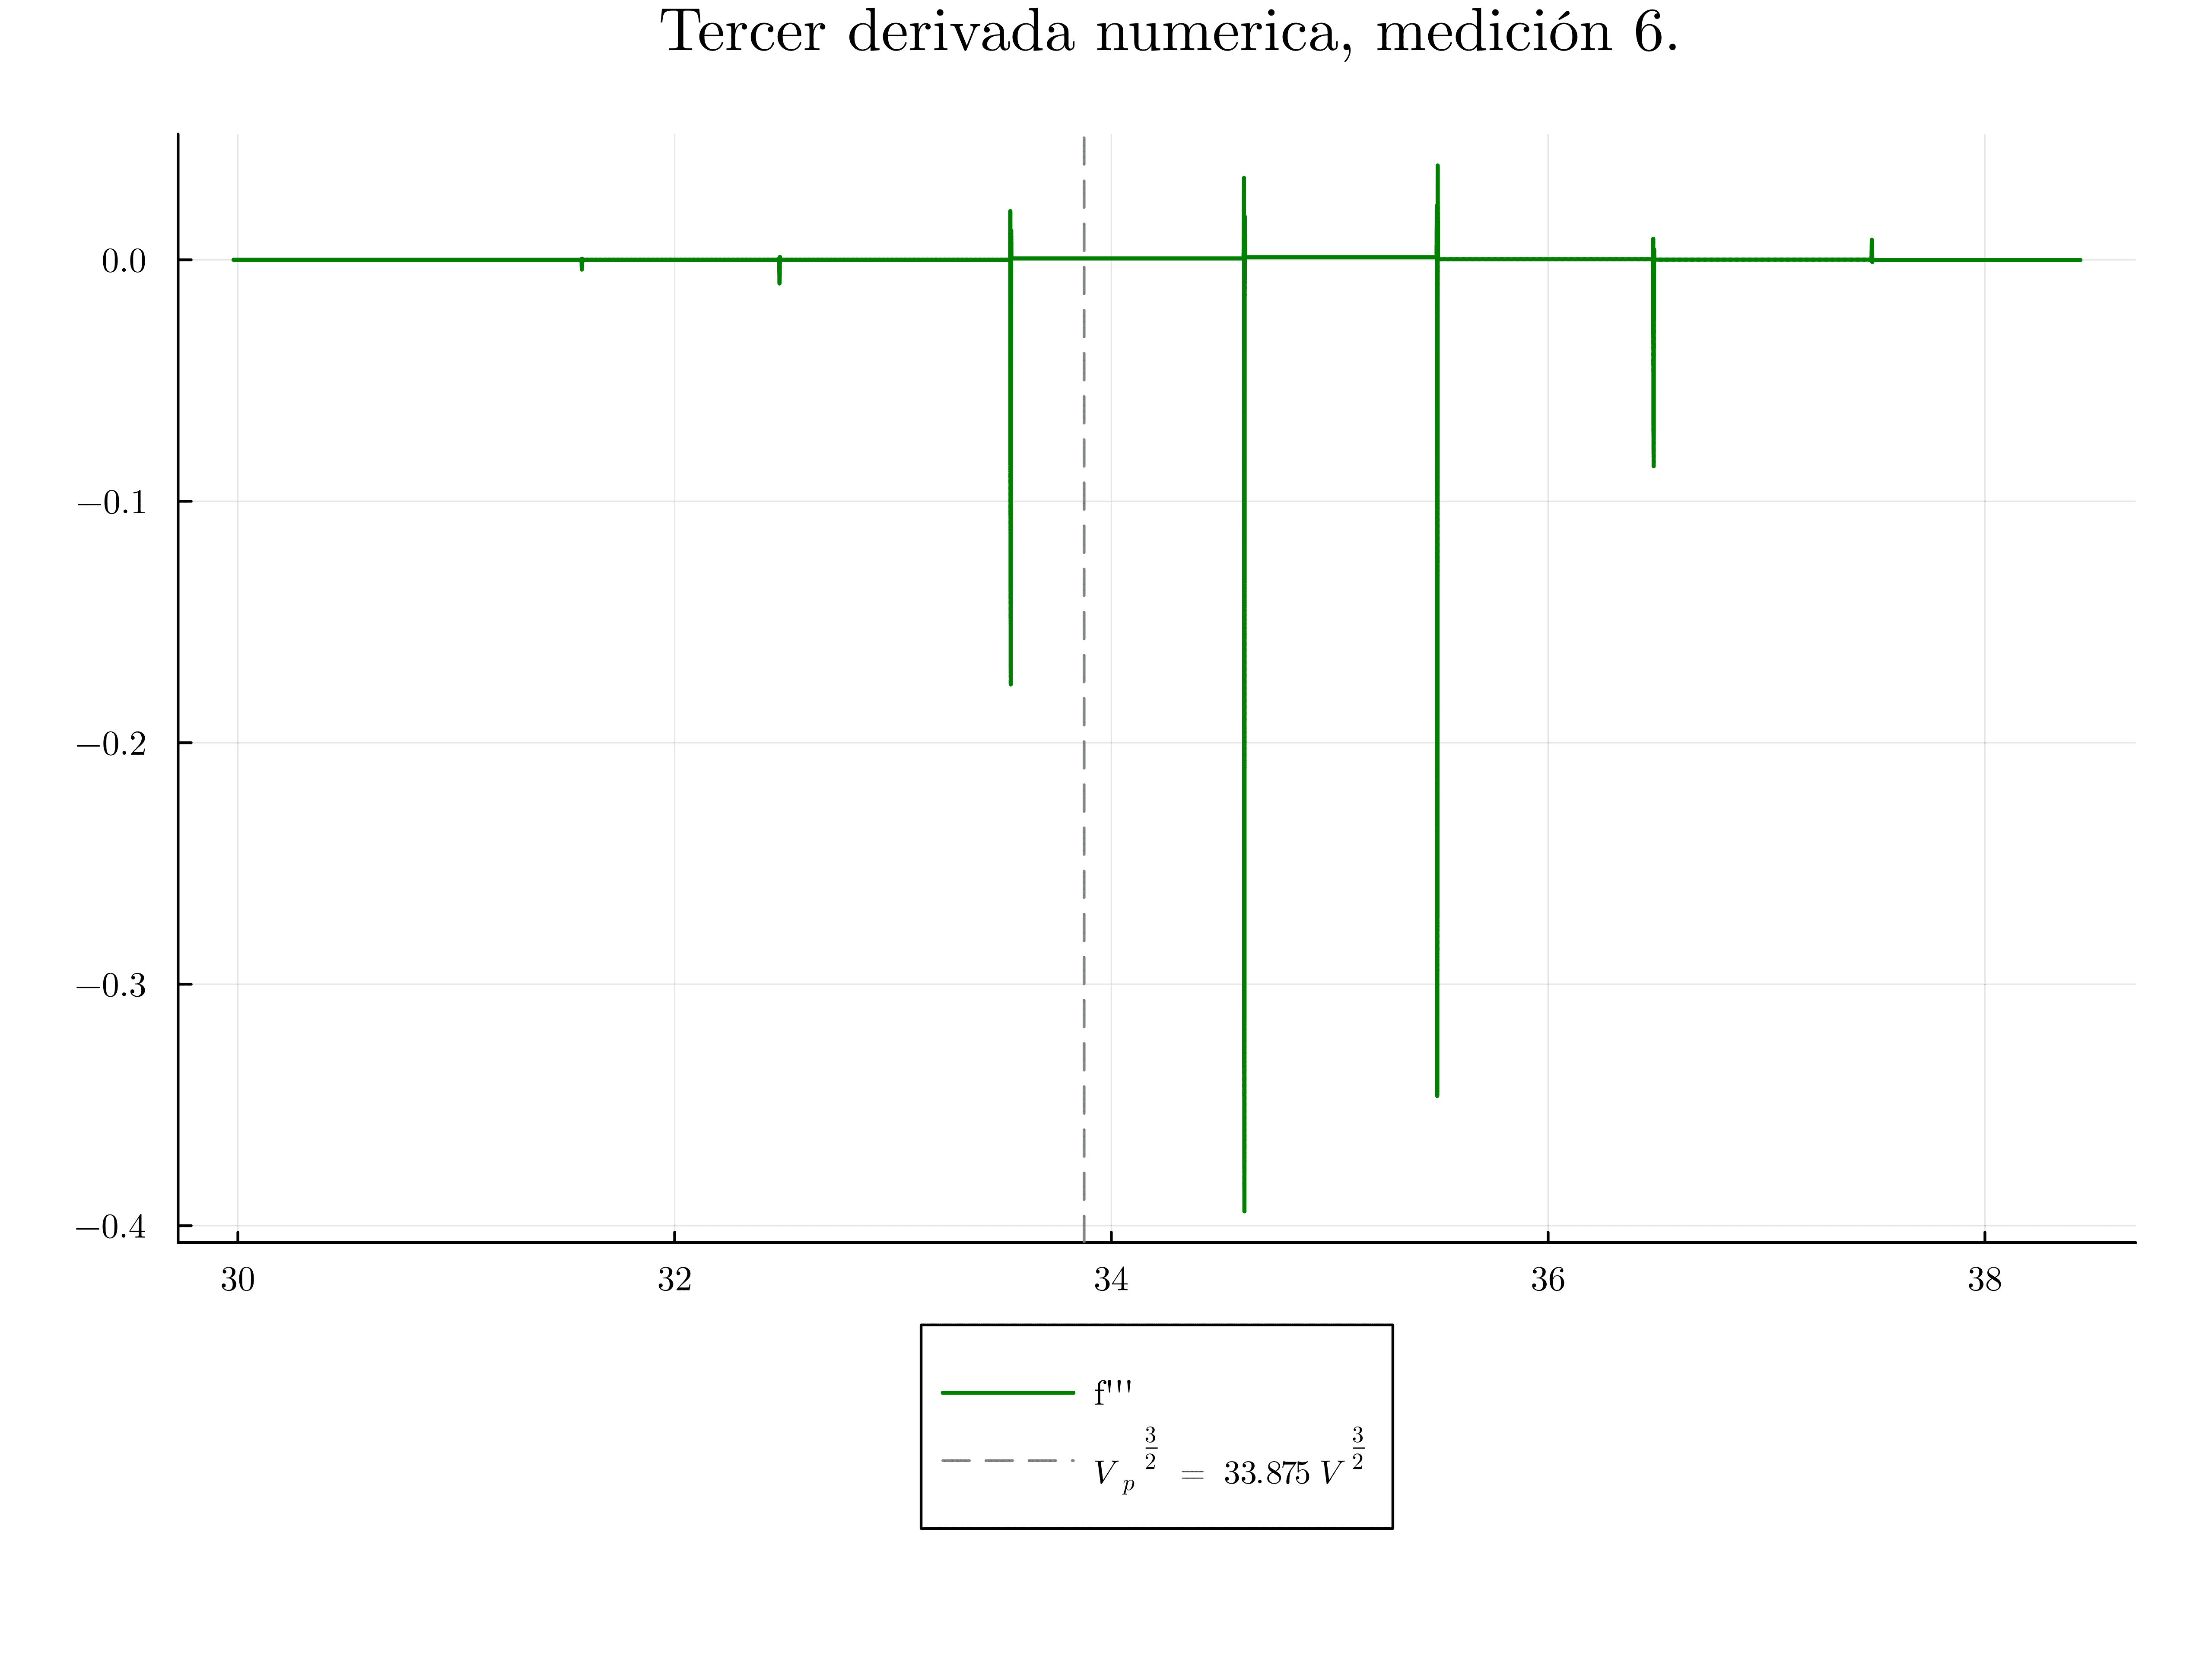
\includegraphics[width=\linewidth]{img/potderst6.png}
		\caption{Barrido n°: 6}
		\label{fig:potderst6}
	\end{subfigure}
	
\end{figure}

% cuarto bloque de figuras
\begin{figure}[H]
	\ContinuedFloat % Indica que esta figura continúa de la anterior
	\centering
	\begin{subfigure}[b]{0.49\textwidth}
		\centering
		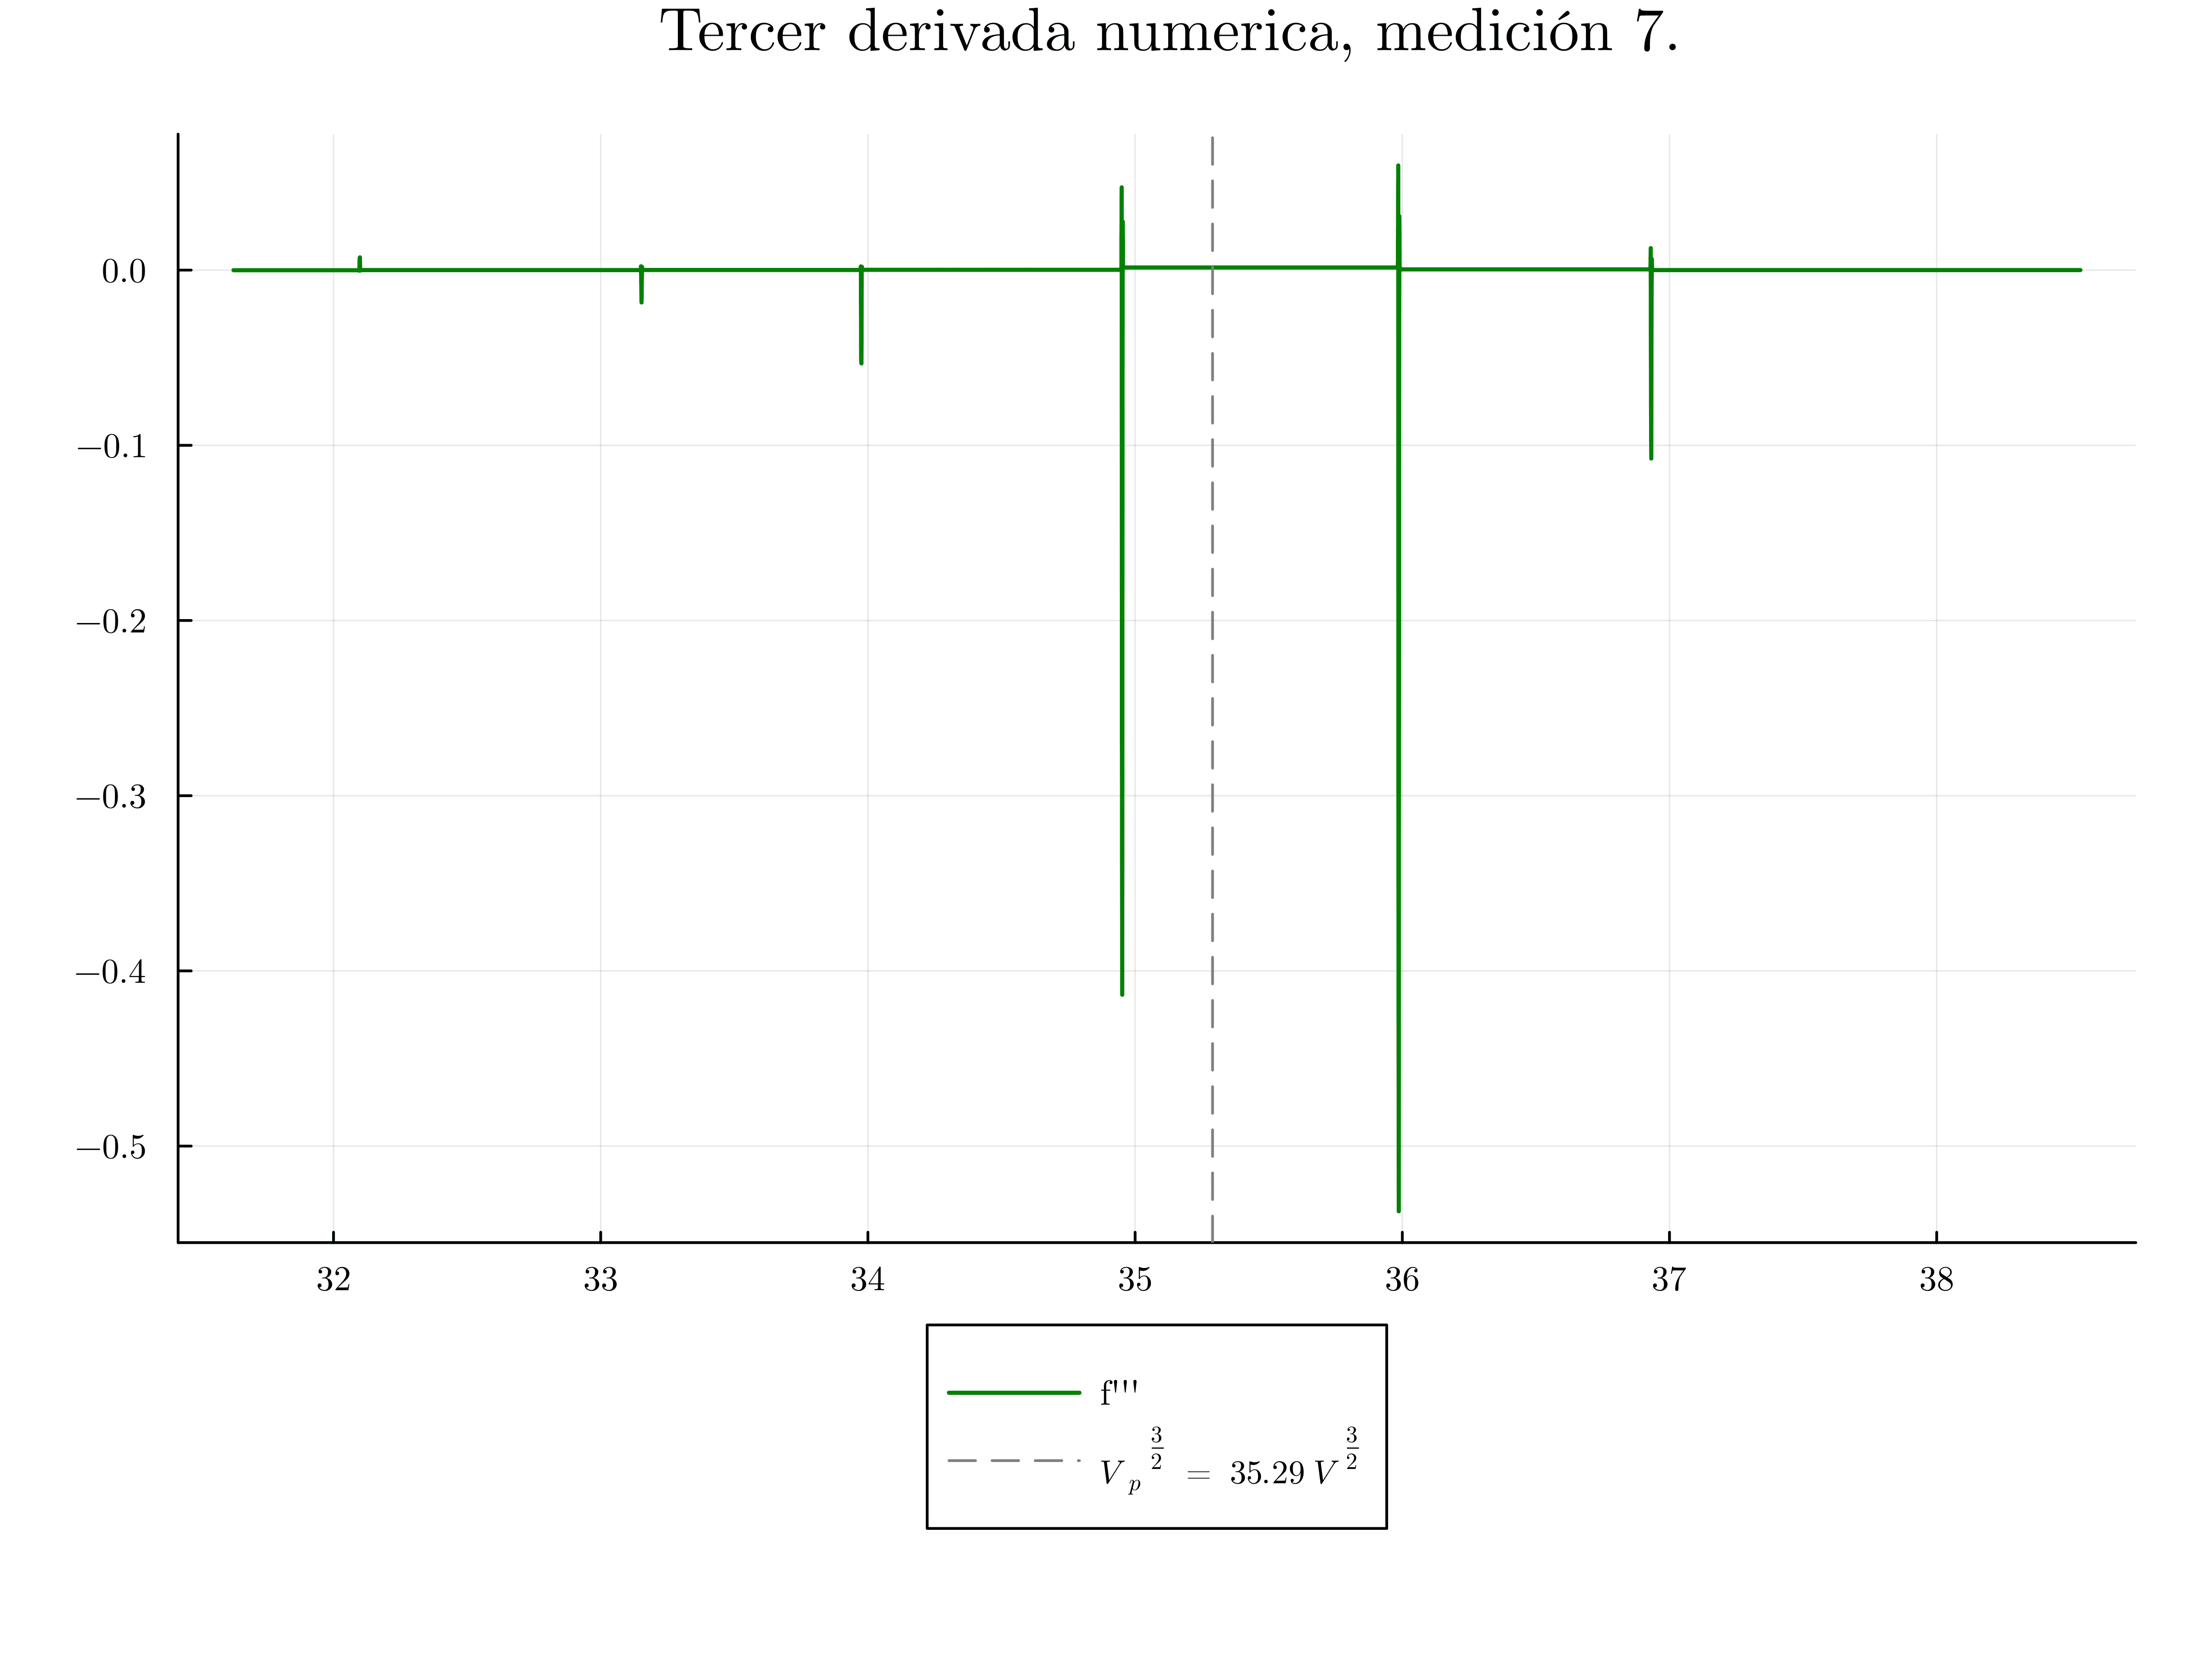
\includegraphics[width=\linewidth]{img/potderst7.png}
		\caption{Barrido n°: 7}
		\label{fig:potderst7}
	\end{subfigure}
	\hfill
	\begin{subfigure}[b]{0.49\textwidth}
		\centering
		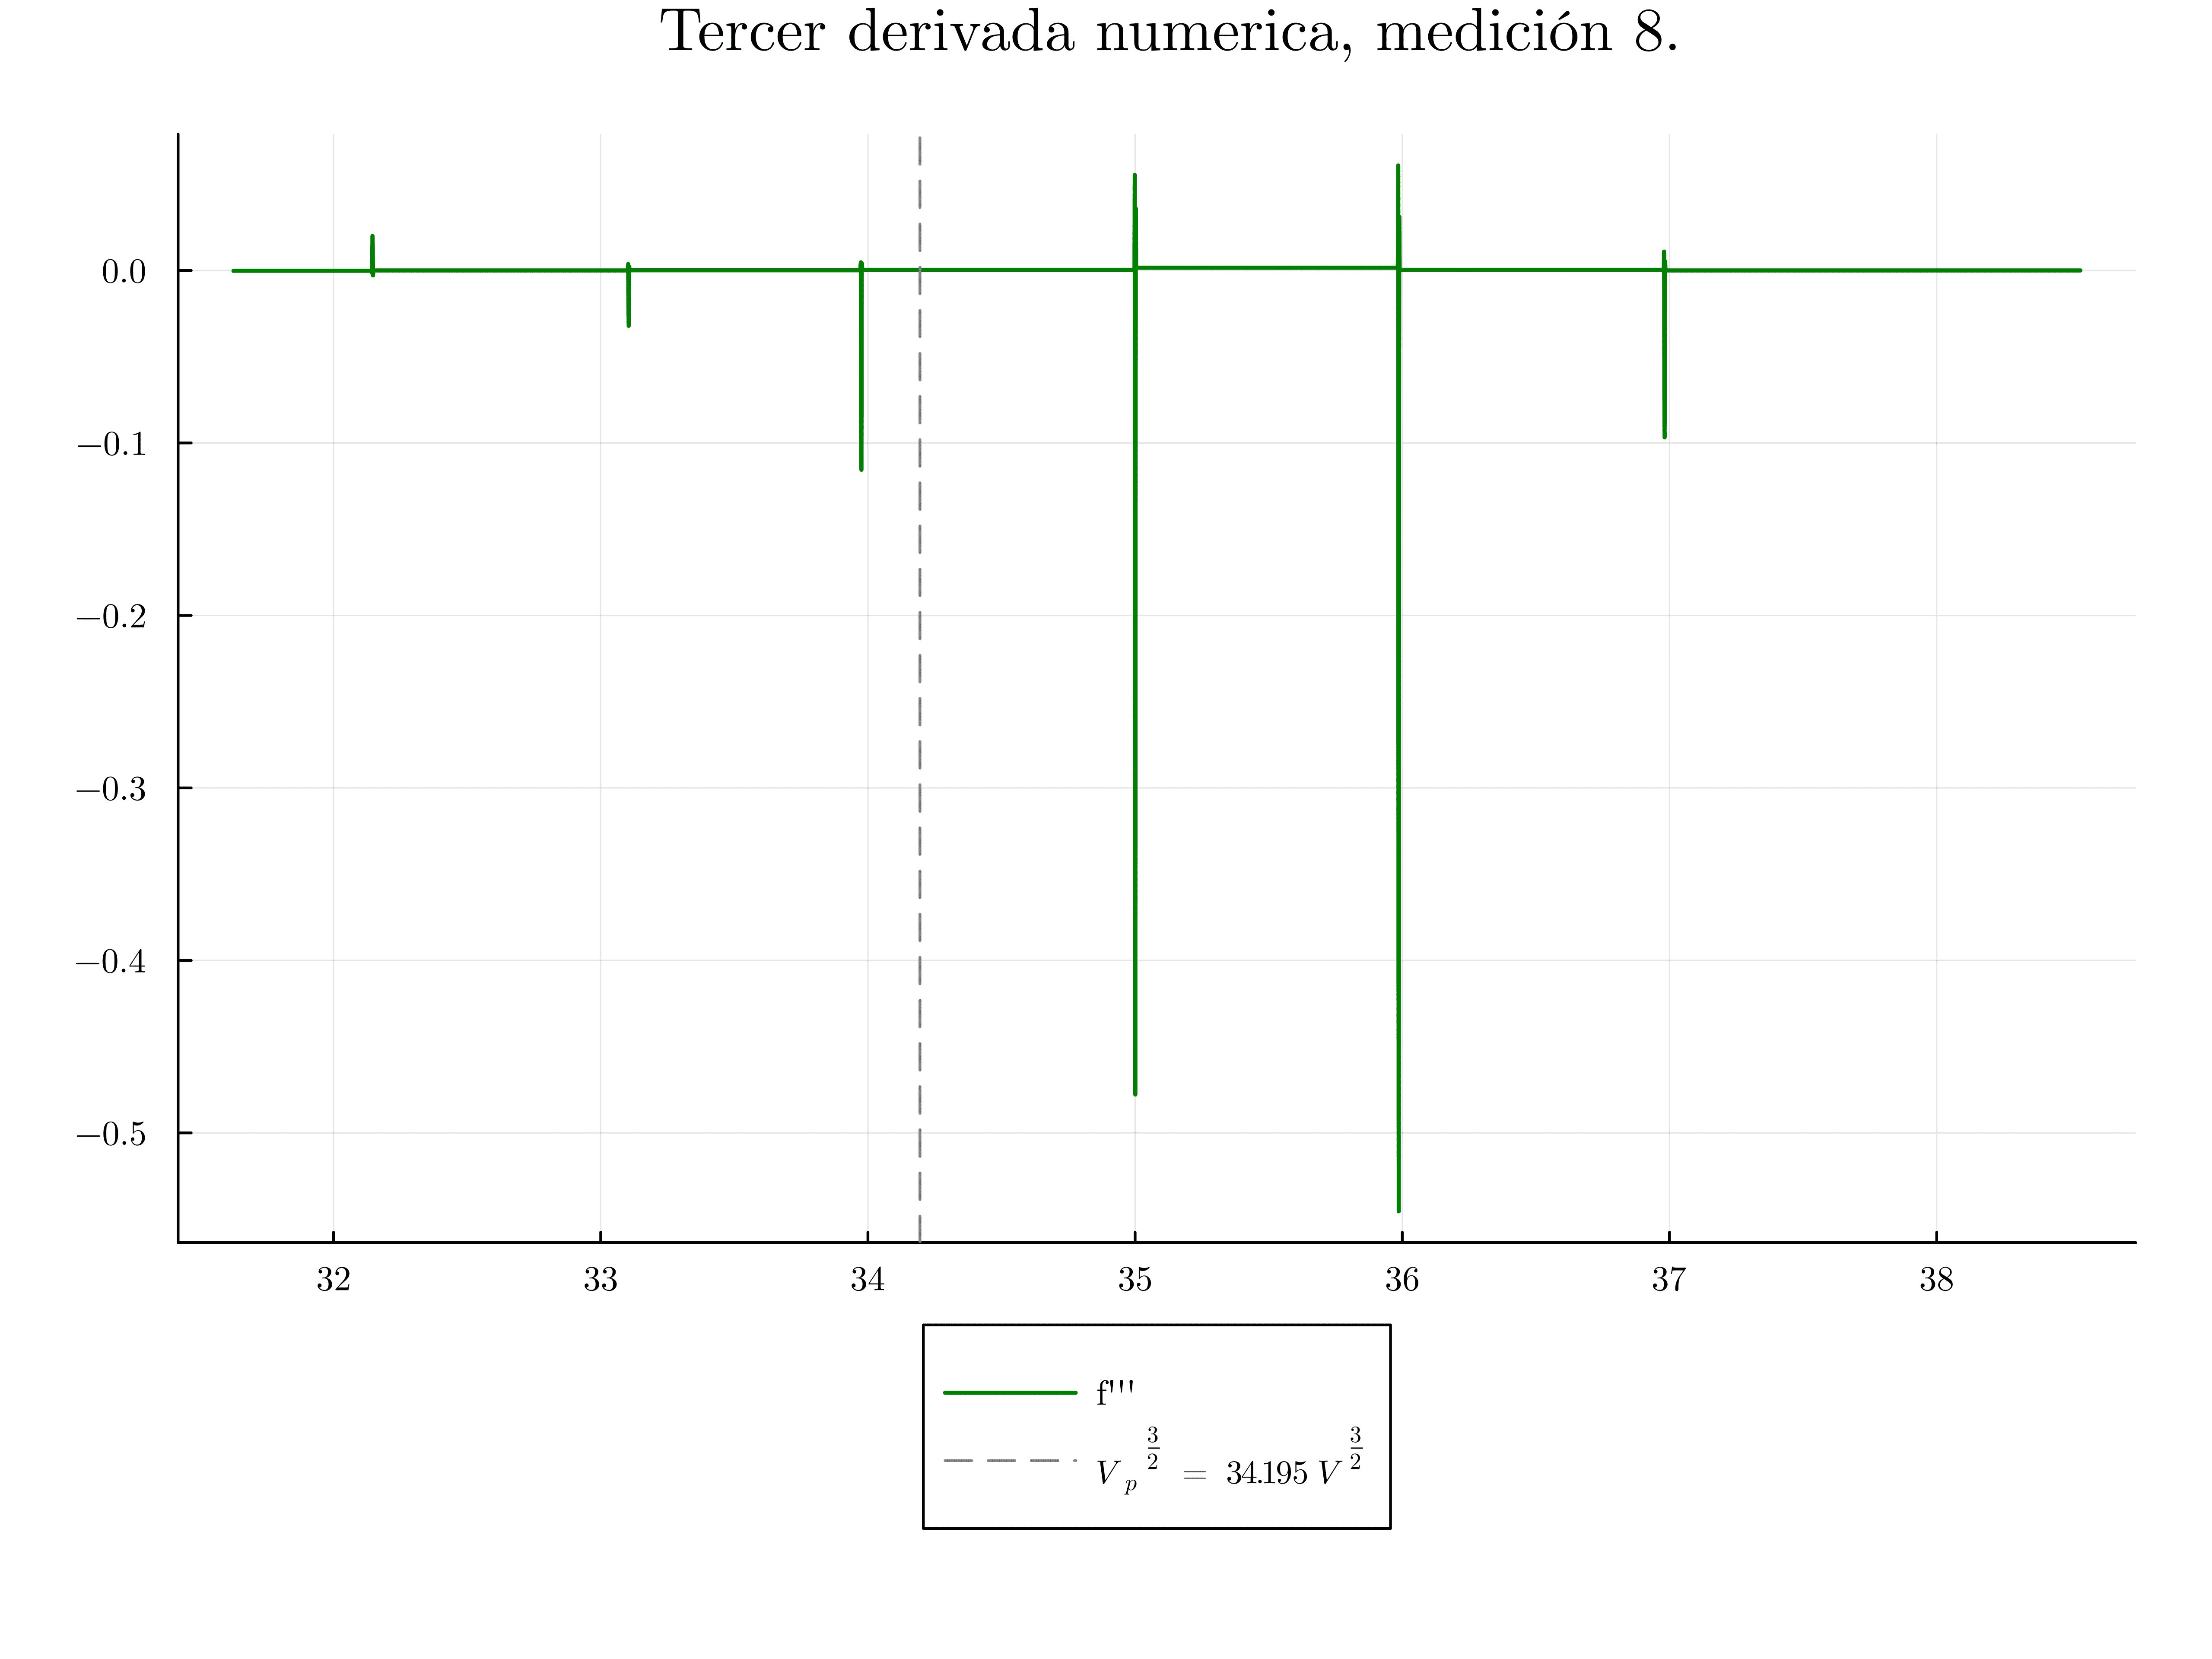
\includegraphics[width=\linewidth]{img/potderst8.png}
		\caption{Barrido n°: 8}
		\label{fig:potderst8}
	\end{subfigure}
\end{figure}


% Últimas figuras
\begin{figure}[H]
	\ContinuedFloat % Sigue con la misma numeración y caption
	\centering
	\begin{subfigure}[b]{0.49\textwidth}
		\centering
		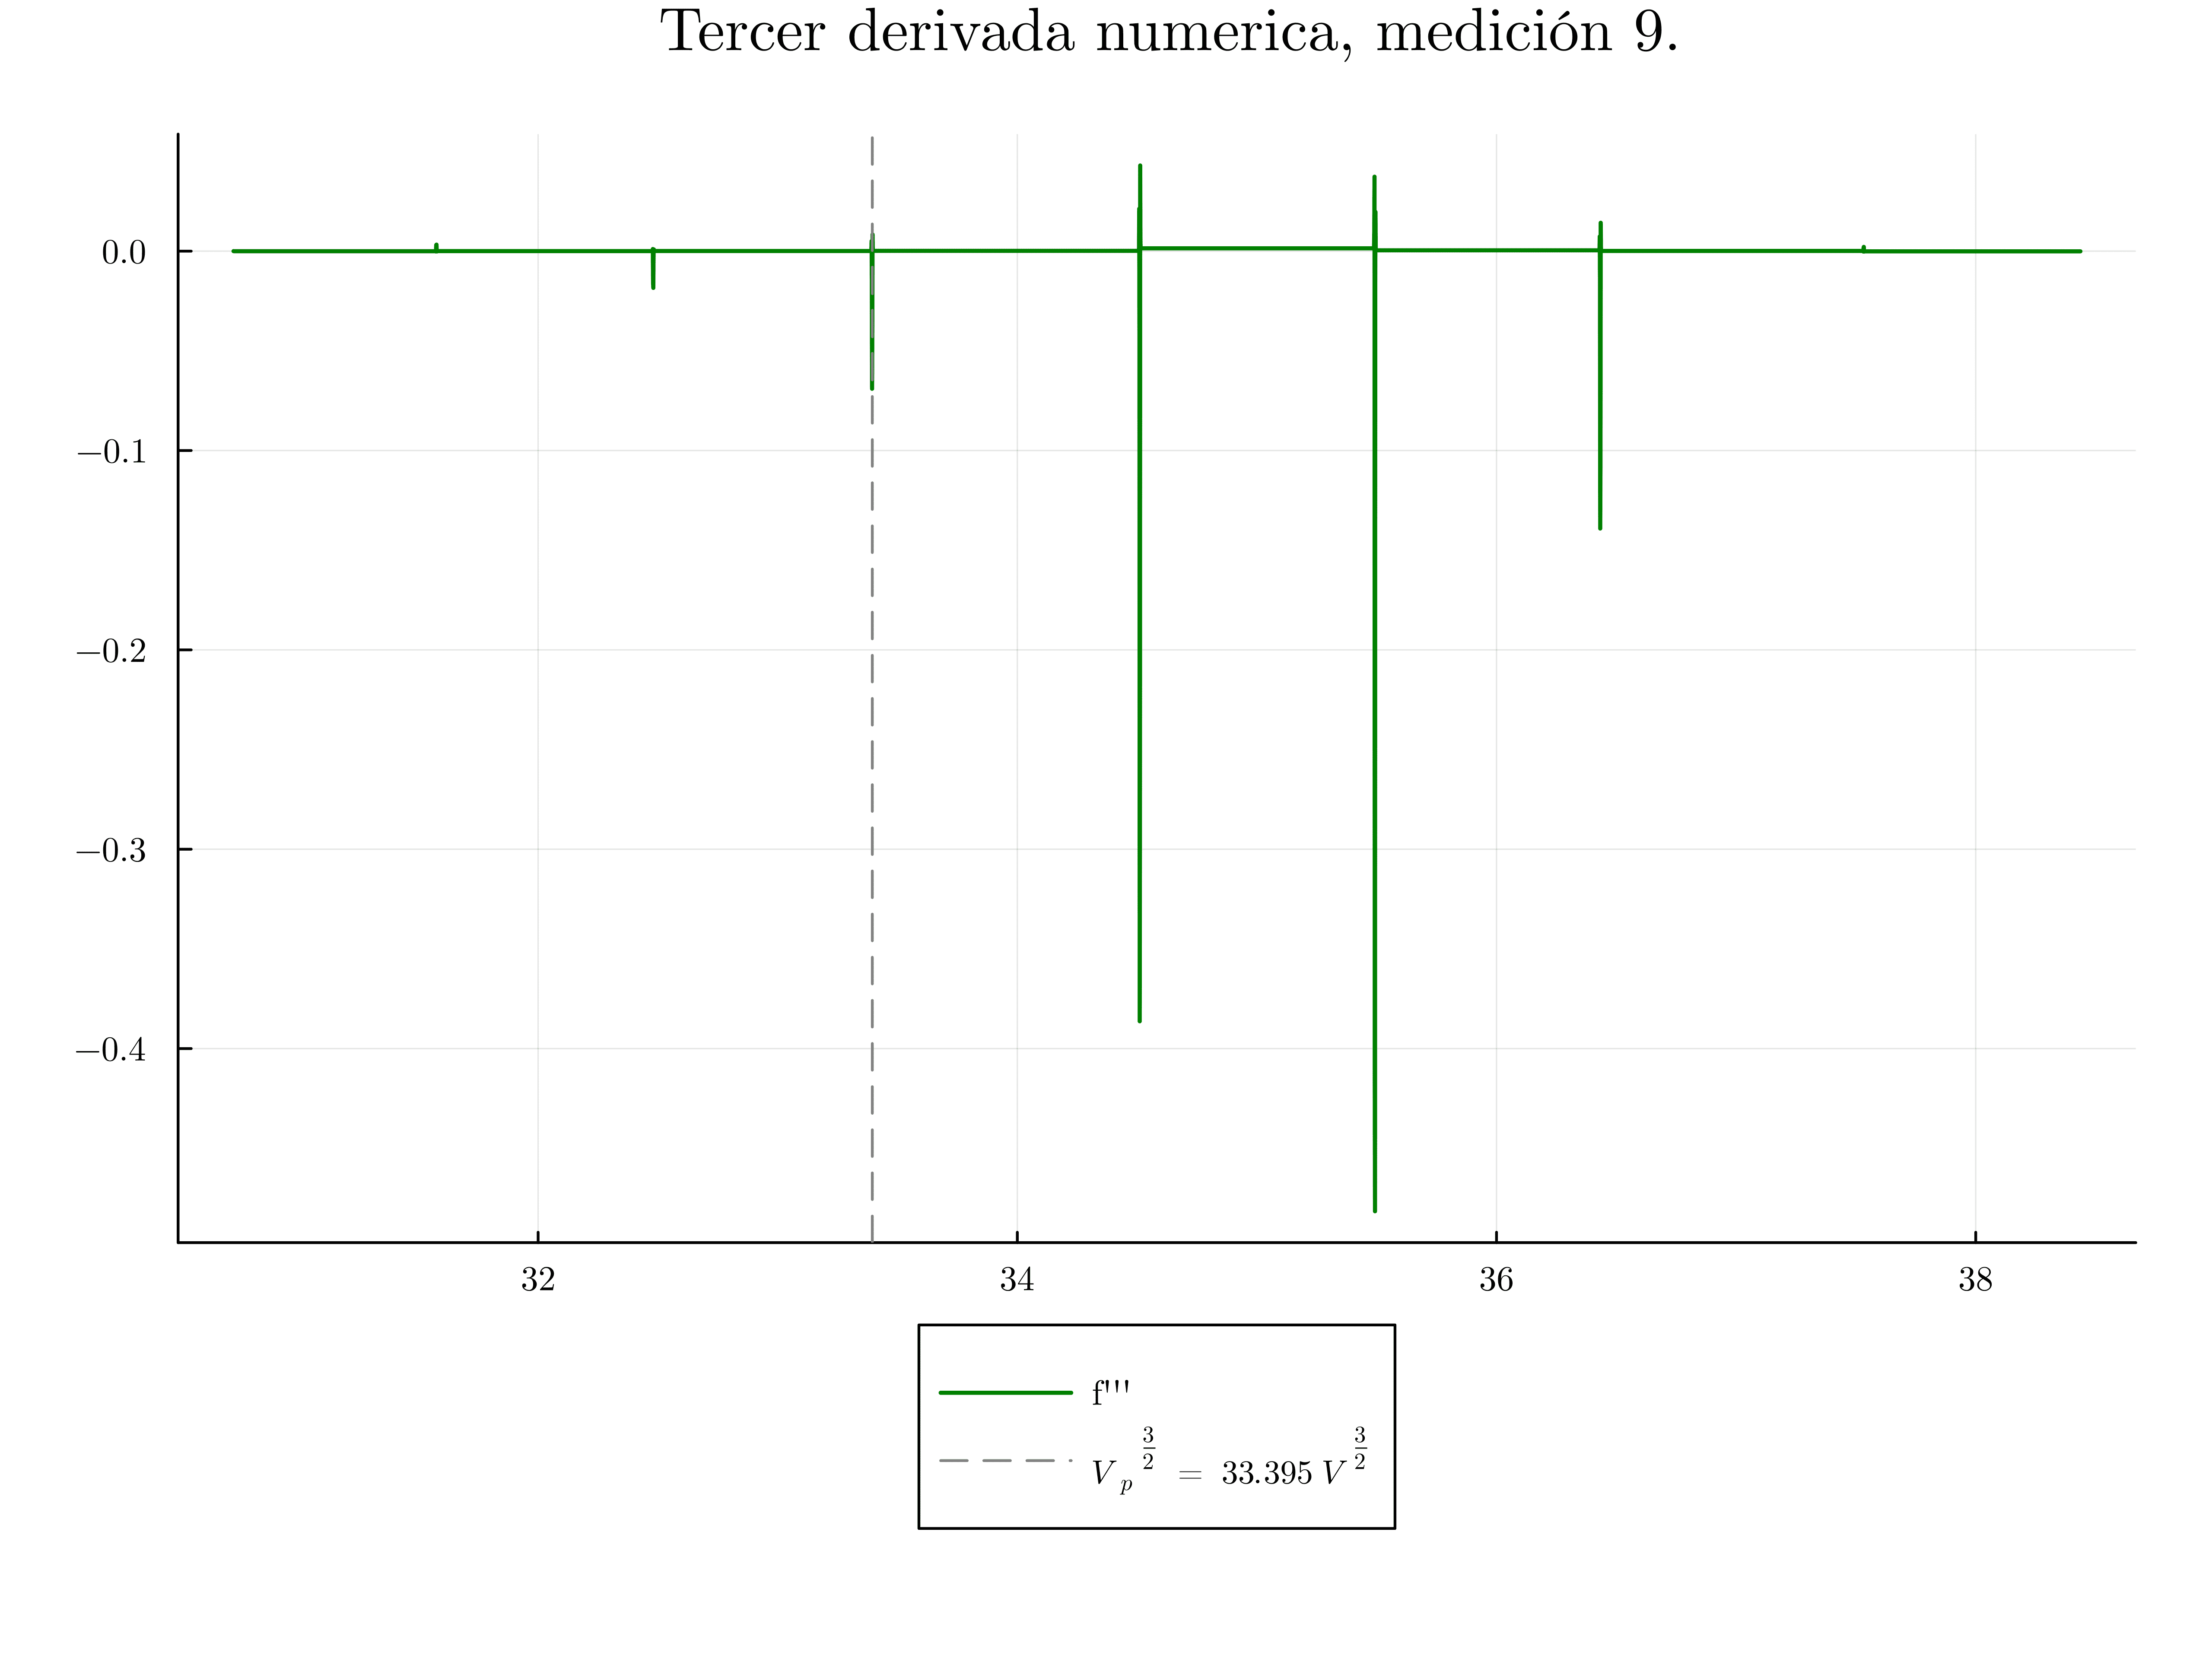
\includegraphics[width=\linewidth]{img/potderst9.png}
		\caption{Barrido n°: 9}
		\label{fig:potderst9}
	\end{subfigure}
	\hfill
	\begin{subfigure}[b]{0.49\textwidth}
		\centering
		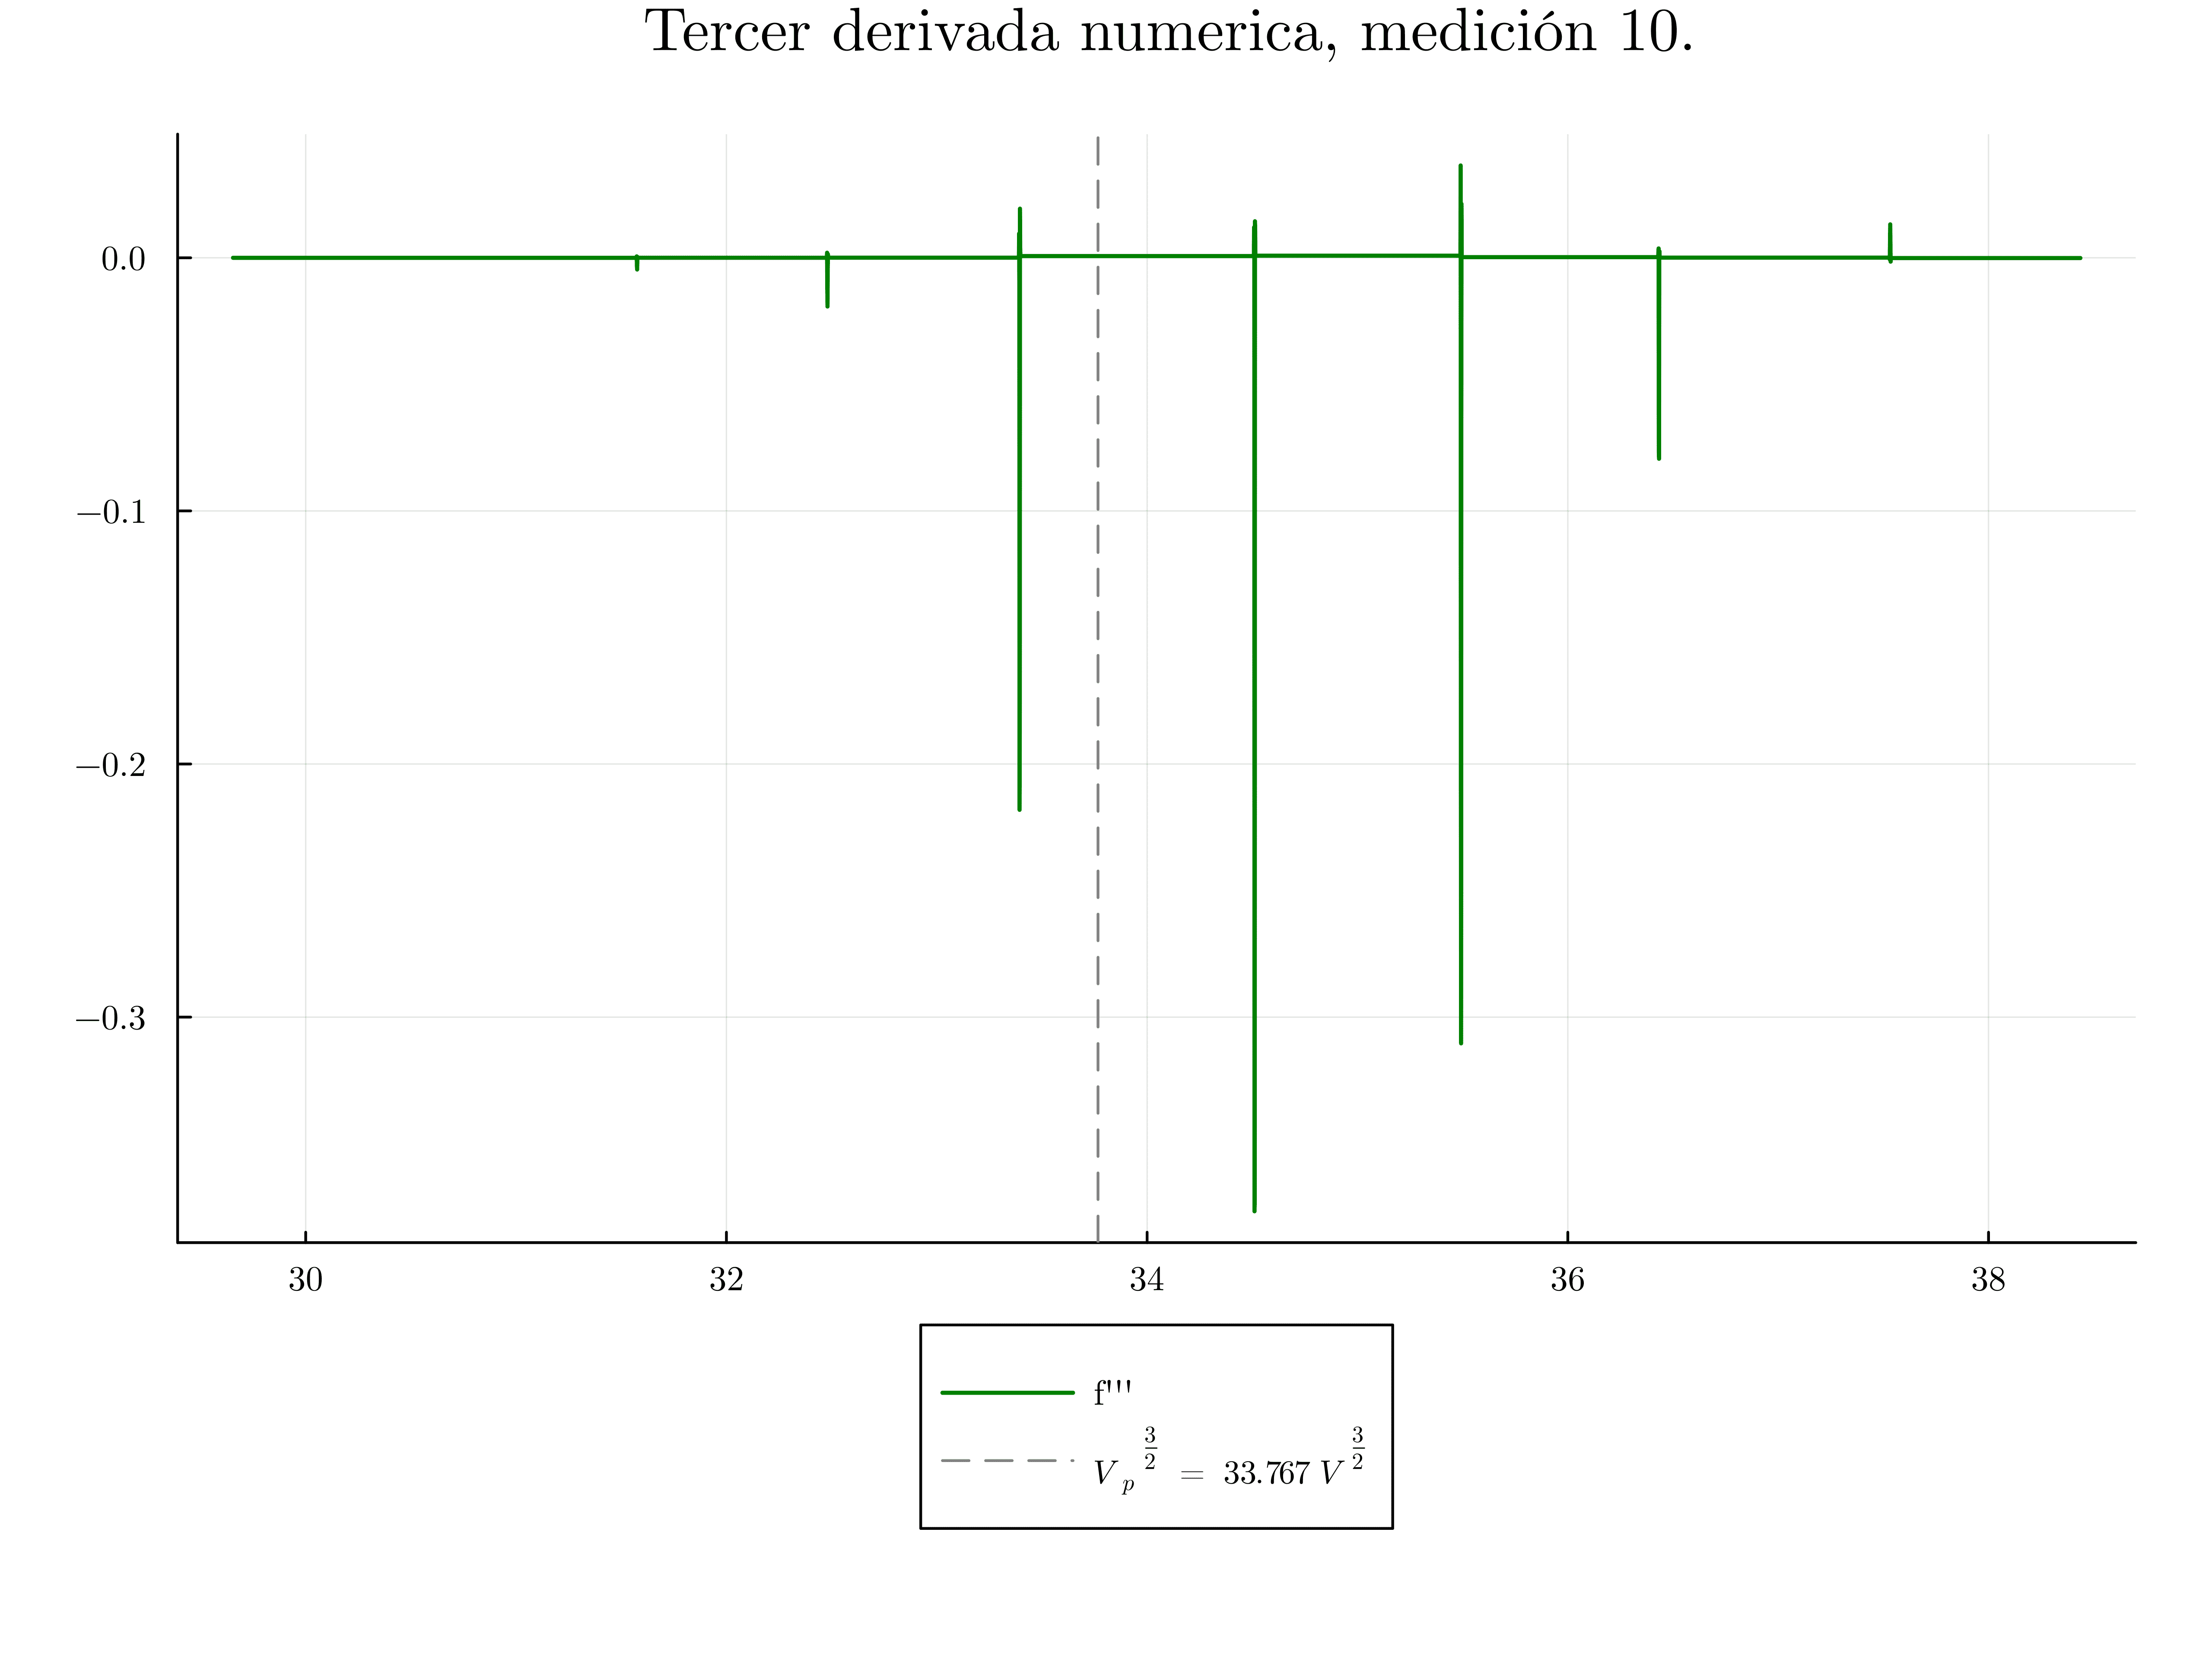
\includegraphics[width=\linewidth]{img/potderst10.png}
		\caption{Barrido n°: 10}
		\label{fig:potderst10}
	\end{subfigure}
	
	\caption{Tercer derivada de la corriente del ánodo con respecto a $V^{\nicefrac{3}{2}}$, para los 10 barridos realizados, donde se puede apreciar, que existen puntos diferentes de cero cuyo valor absoluto es un orden magnitud mayor al del punto elegido (linea gris), por cumplimiento de que que $f^{(2)} = 0$, con tolerancia de $1\times10^{-5}$ y $f^{(3)} \neq 0$, si bien estos puntos podrían ser tomados como puntos de inflexión, al no tener un valor dentro del rango de tolerancia son descartados, a si mismo el cambio tan grande del valor de esta derivada se puede explicar a partir del ruido de la corriente medida el cual se ve trasladado en el algoritmo de LOESS al cambiar en este región múltiples veces de curvatura para ajustar una curva suave }
	\label{fig:potdersts}
\end{figure}

\twocolumngrid


de banco con mayor resolución y precisión como el BK precision 5490C. De aplicarse este diseño, las curvas se podrían promediar debido a que estarían bajo mismas condiciones, a la par de que los puntos serian iguales y directamente se pudiera usar derivación numérica para la determinación del punto de inflexión asociado al voltaje de ionización.
